% !TEX program = pdflatex
% Which mechanisms can drive the rise in Q/Y, and what do the data say about each? 19 Nov 2026.
% Merges the 16 Nov deck (A: Logistics/Discussion_note/29_11_16/slides, AHP total corporate sector)
% and the 18 Nov deck (B: Codes/Calibration_R1/2_Check/2026_11_18_Credit_Buybacks, Z.1 NFC sector).
% Numbers: \va{key} = deck A's value strings, \vb{key} = deck B's, \vc{key} = computed in scripts/build.py.
% An undefined key prints a red ??key, and scripts/build.py fails if any key used here is undefined.
% Colors: blue = data, orange = model, grey = pre-2009 context, green = RoW net purchases.
% Notation colors as in the R1 decks: ink = raw data, purple = constructed from data, orange = implied.
\documentclass[aspectratio=169,10pt,t]{beamer}
\usepackage[T1]{fontenc}
\usepackage[utf8]{inputenc}
\usepackage{lmodern,amsmath,amssymb,booktabs,graphicx,array,xcolor}
\usetheme{default}
\setbeamertemplate{navigation symbols}{}
\setbeamertemplate{footline}{\hfill\textcolor{muted}{\scriptsize\insertframenumber}\hspace{0.4cm}\vspace{0.25cm}}
\setbeamertemplate{itemize items}[circle]
\setbeamertemplate{frametitle}{\vspace{0.3cm}\textbf{\large\insertframetitle}\ifx\insertframesubtitle\empty\else\\[-0.05cm]{\small\textcolor{inksec}{\insertframesubtitle}}\fi\vspace{0.05cm}}
\definecolor{ink}{HTML}{0B0B0B}\definecolor{inksec}{HTML}{52514E}\definecolor{muted}{HTML}{898781}
\definecolor{dataC}{HTML}{2A78D6}\definecolor{dataD}{HTML}{104281}\definecolor{modelC}{HTML}{EB6834}\definecolor{greenC}{HTML}{1BAF7A}\definecolor{washc}{HTML}{F0EFEC}\definecolor{ctxc}{HTML}{C3C2B7}
\definecolor{concol}{HTML}{6F3CC3}\definecolor{impcol}{HTML}{C25E00}
\newcommand{\con}[1]{{\color{concol}#1}}
\newcommand{\imp}[1]{{\color{impcol}#1}}
\setbeamercolor{normal text}{fg=ink,bg=white}\setbeamercolor{structure}{fg=dataD}\setbeamercolor{frametitle}{fg=ink}
\setbeamercolor{block title}{fg=white,bg=dataD}\setbeamercolor{block body}{fg=ink,bg=washc}
\setlength{\leftmargini}{1.1em}
% three value namespaces; an undefined key prints in red instead of silently printing nothing
\newcommand{\vget}[2]{\ifcsname #1:#2\endcsname\csname #1:#2\endcsname\else\textcolor{red}{\textbf{??#1:\detokenize{#2}}}\fi}
\newcommand{\va}[1]{\vget{va}{#1}}% deck A, 16 Nov: AHP total corporate sector
\newcommand{\vb}[1]{\vget{vb}{#1}}% deck B, 18 Nov: Z.1 NFC sector, Compustat
\newcommand{\vc}[1]{\vget{vc}{#1}}% new in this deck
% Deck A (16 Nov 2026, AHP total corporate): verbatim copy of Logistics/Discussion_note/29_11_16/slides/data/values.tex
% Written by scripts/build.py; do not edit. Use \va{key}.
\expandafter\def\csname va:DQ2007\endcsname{3.6}
\expandafter\def\csname va:DQ2009\endcsname{7.4}
\expandafter\def\csname va:DQ2011\endcsname{5.5}
\expandafter\def\csname va:DQ2025\endcsname{2.7}
\expandafter\def\csname va:DY2007\endcsname{8.1}
\expandafter\def\csname va:DY2009\endcsname{14.4}
\expandafter\def\csname va:DY2011\endcsname{12.5}
\expandafter\def\csname va:DY2025\endcsname{12.7}
\expandafter\def\csname va:QY2007\endcsname{2.23}
\expandafter\def\csname va:QY2009\endcsname{1.94}
\expandafter\def\csname va:QY2011\endcsname{2.27}
\expandafter\def\csname va:QY2025\endcsname{4.66}
\expandafter\def\csname va:Y_dtn\endcsname{8.28}
\expandafter\def\csname va:Y_tn2009\endcsname{7.88}
\expandafter\def\csname va:Y_tn2023\endcsname{16.16}
\expandafter\def\csname va:Ymult0923\endcsname{2.05}
\expandafter\def\csname va:avg_cfctax\endcsname{26.4}
\expandafter\def\csname va:avg_comp\endcsname{57.3}
\expandafter\def\csname va:avg_fcf\endcsname{12.4}
\expandafter\def\csname va:avg_ncf\endcsname{3.9}
\expandafter\def\csname va:avg_nonlab\endcsname{42.7}
\expandafter\def\csname va:dDY2007\endcsname{0.45}
\expandafter\def\csname va:dDY2009\endcsname{\ensuremath{-}0.13}
\expandafter\def\csname va:dDY2011\endcsname{0.01}
\expandafter\def\csname va:dDY2013\endcsname{0.10}
\expandafter\def\csname va:dQD2007\endcsname{0.29}
\expandafter\def\csname va:dQD2009\endcsname{1.01}
\expandafter\def\csname va:dQD2011\endcsname{0.71}
\expandafter\def\csname va:dQD2013\endcsname{0.33}
\expandafter\def\csname va:dQY2007\endcsname{0.74}
\expandafter\def\csname va:dQY2009\endcsname{0.88}
\expandafter\def\csname va:dQY2011\endcsname{0.72}
\expandafter\def\csname va:dQY2013\endcsname{0.43}
\expandafter\def\csname va:feBHQ2009\endcsname{0.153}
\expandafter\def\csname va:feBHQ2023\endcsname{0.082}
\expandafter\def\csname va:feBHQcf2023\endcsname{0.222}
\expandafter\def\csname va:feBHQratio2023\endcsname{37}
\expandafter\def\csname va:feHmult\endcsname{1.45}
\expandafter\def\csname va:feaIdx2023\endcsname{0.37}
\expandafter\def\csname va:feaSlope\endcsname{\ensuremath{-}6.6}
\expandafter\def\csname va:g_cfctax_contrib\endcsname{26}
\expandafter\def\csname va:g_cfctax_mult\endcsname{2.00}
\expandafter\def\csname va:g_cfctax_sh2009\endcsname{27.2}
\expandafter\def\csname va:g_cfctax_sh2023\endcsname{26.6}
\expandafter\def\csname va:g_fcf_contrib\endcsname{11}
\expandafter\def\csname va:g_fcf_dtn\endcsname{0.92}
\expandafter\def\csname va:g_fcf_mult\endcsname{1.81}
\expandafter\def\csname va:g_fcf_sh2009\endcsname{14.4}
\expandafter\def\csname va:g_fcf_sh2023\endcsname{12.7}
\expandafter\def\csname va:g_fcf_tn2009\endcsname{1.14}
\expandafter\def\csname va:g_fcf_tn2023\endcsname{2.06}
\expandafter\def\csname va:g_kap_contrib\endcsname{35}
\expandafter\def\csname va:g_kap_dtn\endcsname{2.93}
\expandafter\def\csname va:g_kap_sh2009\endcsname{26.6}
\expandafter\def\csname va:g_kap_sh2023\endcsname{31.1}
\expandafter\def\csname va:g_kap_tn2009\endcsname{2.10}
\expandafter\def\csname va:g_kap_tn2023\endcsname{5.03}
\expandafter\def\csname va:g_ncf_contrib\endcsname{9}
\expandafter\def\csname va:g_ncf_mult\endcsname{nan}
\expandafter\def\csname va:g_ncf_sh2009\endcsname{\ensuremath{-}0.6}
\expandafter\def\csname va:g_ncf_sh2023\endcsname{4.5}
\expandafter\def\csname va:g_skilled_contrib\endcsname{34}
\expandafter\def\csname va:g_skilled_dtn\endcsname{2.80}
\expandafter\def\csname va:g_skilled_mult\endcsname{2.20}
\expandafter\def\csname va:g_skilled_sh2009\endcsname{29.6}
\expandafter\def\csname va:g_skilled_sh2023\endcsname{31.8}
\expandafter\def\csname va:g_skilled_tn2009\endcsname{2.33}
\expandafter\def\csname va:g_skilled_tn2023\endcsname{5.13}
\expandafter\def\csname va:g_unskilled_contrib\endcsname{20}
\expandafter\def\csname va:g_unskilled_dtn\endcsname{1.63}
\expandafter\def\csname va:g_unskilled_mult\endcsname{1.71}
\expandafter\def\csname va:g_unskilled_sh2009\endcsname{29.3}
\expandafter\def\csname va:g_unskilled_sh2023\endcsname{24.4}
\expandafter\def\csname va:g_unskilled_tn2009\endcsname{2.31}
\expandafter\def\csname va:g_unskilled_tn2023\endcsname{3.94}
\expandafter\def\csname va:inctax2009\endcsname{2.6}
\expandafter\def\csname va:inctax2023\endcsname{3.8}
\expandafter\def\csname va:k_BH_gr\endcsname{5.5}
\expandafter\def\csname va:k_BH_mult\endcsname{2.12}
\expandafter\def\csname va:k_BL_gr\endcsname{3.6}
\expandafter\def\csname va:k_BL_mult\endcsname{1.64}
\expandafter\def\csname va:k_H_gr\endcsname{2.7}
\expandafter\def\csname va:k_H_mult\endcsname{1.45}
\expandafter\def\csname va:k_L_gr\endcsname{0.6}
\expandafter\def\csname va:k_L_mult\endcsname{1.09}
\expandafter\def\csname va:k_prem2009\endcsname{2.29}
\expandafter\def\csname va:k_prem2013\endcsname{2.40}
\expandafter\def\csname va:k_prem2023\endcsname{2.21}
\expandafter\def\csname va:k_prem2024\endcsname{2.97}
\expandafter\def\csname va:k_wH2009\endcsname{107}
\expandafter\def\csname va:k_wH2023\endcsname{156}
\expandafter\def\csname va:k_wH_gr\endcsname{2.7}
\expandafter\def\csname va:k_wH_mult\endcsname{1.46}
\expandafter\def\csname va:k_wL_gr\endcsname{3.0}
\expandafter\def\csname va:k_wL_mult\endcsname{1.51}
\expandafter\def\csname va:mDY100\endcsname{\ensuremath{-}2.79}
\expandafter\def\csname va:mQY100\endcsname{\ensuremath{-}0.54}
\expandafter\def\csname va:ncf2009\endcsname{\ensuremath{-}0.6}
\expandafter\def\csname va:ncf2025\endcsname{4.0}
\expandafter\def\csname va:nonlab2009\endcsname{41.1}
\expandafter\def\csname va:nonlab2025\endcsname{44.1}
\expandafter\def\csname va:shDYofQY2007\endcsname{60}
\expandafter\def\csname va:shDYofQY2009\endcsname{\ensuremath{-}15}
\expandafter\def\csname va:shDYofQY2011\endcsname{2}
\expandafter\def\csname va:shDYofQY2013\endcsname{23}
\expandafter\def\csname va:shQY2007\endcsname{252}
\expandafter\def\csname va:shQY2009\endcsname{87}
\expandafter\def\csname va:shQY2011\endcsname{102}
\expandafter\def\csname va:shQY2013\endcsname{130}
\expandafter\def\csname va:sk2009\endcsname{50}
\expandafter\def\csname va:sk2023\endcsname{57}
\expandafter\def\csname va:sp_bls2009\endcsname{1.82}
\expandafter\def\csname va:sp_bls2022\endcsname{1.81}
\expandafter\def\csname va:sp_bls2023\endcsname{1.79}
\expandafter\def\csname va:sp_bls2024\endcsname{1.82}
\expandafter\def\csname va:sp_bls_max\endcsname{1.83}
\expandafter\def\csname va:sp_bls_min\endcsname{1.79}
\expandafter\def\csname va:sp_par2009\endcsname{2.05}
\expandafter\def\csname va:sp_par2022\endcsname{2.23}
\expandafter\def\csname va:sp_par2023\endcsname{2.18}
\expandafter\def\csname va:sp_par2024\endcsname{2.15}
\expandafter\def\csname va:sp_pkg2009\endcsname{1.874}
\expandafter\def\csname va:sp_pkg2022\endcsname{1.800}
\expandafter\def\csname va:sp_pkg2023\endcsname{1.917}
\expandafter\def\csname va:sp_pkg2024\endcsname{2.159}
\expandafter\def\csname va:sp_pkg_jump\endcsname{20}
\expandafter\def\csname va:sp_rc2009\endcsname{1.874}
\expandafter\def\csname va:sp_rc2022\endcsname{1.800}
\expandafter\def\csname va:sp_rc2023\endcsname{1.780}
\expandafter\def\csname va:sp_rc2024\endcsname{1.779}
\expandafter\def\csname va:ss_acs2009\endcsname{47}
\expandafter\def\csname va:ss_acs2023\endcsname{58}
\expandafter\def\csname va:ss_cps2009\endcsname{40}
\expandafter\def\csname va:ss_cps2023\endcsname{50}
\expandafter\def\csname va:ss_klems2009\endcsname{50}
\expandafter\def\csname va:ss_klems2023\endcsname{57}
\expandafter\def\csname va:ss_stem2011\endcsname{11}
\expandafter\def\csname va:ss_stem2023\endcsname{14}
\expandafter\def\csname va:x_EL2009\endcsname{5.4}
\expandafter\def\csname va:x_EL2011\endcsname{6.8}
\expandafter\def\csname va:x_EL2025\endcsname{40.7}
\expandafter\def\csname va:x_gain_post\endcsname{12.2}
\expandafter\def\csname va:x_gain_pre\endcsname{1.7}
\expandafter\def\csname va:x_gain_sh2009\endcsname{74}
\expandafter\def\csname va:x_gain_sh2011\endcsname{76}
\expandafter\def\csname va:x_gva\endcsname{2.30}
\expandafter\def\csname va:x_other_sh2009\endcsname{8}
\expandafter\def\csname va:x_other_sh2011\endcsname{7}
\expandafter\def\csname va:x_pA\endcsname{1.82}
\expandafter\def\csname va:x_pL\endcsname{4.07}
\expandafter\def\csname va:x_purch_post\endcsname{3.5}
\expandafter\def\csname va:x_purch_pre\endcsname{3.4}
\expandafter\def\csname va:x_purch_sh2009\endcsname{19}
\expandafter\def\csname va:x_purch_sh2011\endcsname{17}
\expandafter\def\csname va:x_qtyL\endcsname{1.84}
\expandafter\def\csname va:z2007\endcsname{1.04}
\expandafter\def\csname va:z2009\endcsname{1.21}
\expandafter\def\csname va:z2011\endcsname{1.29}
\expandafter\def\csname va:z2025\endcsname{1.32}
\expandafter\def\csname va:zjun2025\endcsname{1.40}
\expandafter\def\csname va:zmean\endcsname{1.29}
\expandafter\def\csname va:zmin_all\endcsname{1.02}
\expandafter\def\csname va:zslope\endcsname{0.9}

% Deck B (18 Nov 2026, Z.1 NFC): verbatim copy of Codes/Calibration_R1/2_Check/2026_11_18_Credit_Buybacks/data/values.tex
% Written by scripts/build.py; do not edit. Use \vb{key}.
\expandafter\def\csname vb:vintage_fcf_diff\endcsname{0.00}
\expandafter\def\csname vb:vintage_q_diff\endcsname{0.00}
\expandafter\def\csname vb:latest_q\endcsname{2026Q2}
\expandafter\def\csname vb:lat_QY\endcsname{546}
\expandafter\def\csname vb:lat_DEBTY\endcsname{97.0}
\expandafter\def\csname vb:lat_KY\endcsname{203}
\expandafter\def\csname vb:lat_PCY\endcsname{6.93}
\expandafter\def\csname vb:lat_EQY\endcsname{586}
\expandafter\def\csname vb:lat_q\endcsname{2.70}
\expandafter\def\csname vb:lat_NB_ttm\endcsname{826}
\expandafter\def\csname vb:lat_NBY\endcsname{5.10}
\expandafter\def\csname vb:lat_BUYY\endcsname{-0.19}
\expandafter\def\csname vb:lat_NCFY\endcsname{3.82}
\expandafter\def\csname vb:QY1990\endcsname{143}
\expandafter\def\csname vb:EQY1990\endcsname{107}
\expandafter\def\csname vb:DEBTY1990\endcsname{82.7}
\expandafter\def\csname vb:BONDSY1990\endcsname{39.7}
\expandafter\def\csname vb:LOANSY1990\endcsname{43.0}
\expandafter\def\csname vb:PCY1990\endcsname{0.00}
\expandafter\def\csname vb:KY1990\endcsname{210}
\expandafter\def\csname vb:REY1990\endcsname{106}
\expandafter\def\csname vb:EQPY1990\endcsname{57.5}
\expandafter\def\csname vb:IPPY1990\endcsname{15.4}
\expandafter\def\csname vb:INVY1990\endcsname{28.8}
\expandafter\def\csname vb:FCFY1990\endcsname{7.12}
\expandafter\def\csname vb:DEQY1990\endcsname{5.74}
\expandafter\def\csname vb:DIVY1990\endcsname{3.74}
\expandafter\def\csname vb:BUYY1990\endcsname{2.00}
\expandafter\def\csname vb:NBY1990\endcsname{4.23}
\expandafter\def\csname vb:NCFY1990\endcsname{4.22}
\expandafter\def\csname vb:q1990\endcsname{0.68}
\expandafter\def\csname vb:Y_tn1990\endcsname{3.16}
\expandafter\def\csname vb:Q_tn1990\endcsname{4.53}
\expandafter\def\csname vb:DEBT_tn1990\endcsname{2.61}
\expandafter\def\csname vb:QY2000\endcsname{258}
\expandafter\def\csname vb:EQY2000\endcsname{280}
\expandafter\def\csname vb:DEBTY2000\endcsname{87.6}
\expandafter\def\csname vb:BONDSY2000\endcsname{49.9}
\expandafter\def\csname vb:LOANSY2000\endcsname{37.7}
\expandafter\def\csname vb:PCY2000\endcsname{0.00}
\expandafter\def\csname vb:KY2000\endcsname{198}
\expandafter\def\csname vb:REY2000\endcsname{98.4}
\expandafter\def\csname vb:EQPY2000\endcsname{52.5}
\expandafter\def\csname vb:IPPY2000\endcsname{19.7}
\expandafter\def\csname vb:INVY2000\endcsname{24.3}
\expandafter\def\csname vb:FCFY2000\endcsname{2.68}
\expandafter\def\csname vb:DEQY2000\endcsname{5.21}
\expandafter\def\csname vb:DIVY2000\endcsname{4.56}
\expandafter\def\csname vb:BUYY2000\endcsname{0.65}
\expandafter\def\csname vb:NBY2000\endcsname{6.37}
\expandafter\def\csname vb:NCFY2000\endcsname{7.50}
\expandafter\def\csname vb:q2000\endcsname{1.30}
\expandafter\def\csname vb:Y_tn2000\endcsname{5.51}
\expandafter\def\csname vb:Q_tn2000\endcsname{14.2}
\expandafter\def\csname vb:DEBT_tn2000\endcsname{4.83}
\expandafter\def\csname vb:QY2007\endcsname{235}
\expandafter\def\csname vb:EQY2007\endcsname{269}
\expandafter\def\csname vb:DEBTY2007\endcsname{91.5}
\expandafter\def\csname vb:BONDSY2007\endcsname{47.8}
\expandafter\def\csname vb:LOANSY2007\endcsname{43.8}
\expandafter\def\csname vb:PCY2007\endcsname{0.00}
\expandafter\def\csname vb:KY2007\endcsname{241}
\expandafter\def\csname vb:REY2007\endcsname{138}
\expandafter\def\csname vb:EQPY2007\endcsname{50.2}
\expandafter\def\csname vb:IPPY2007\endcsname{21.4}
\expandafter\def\csname vb:INVY2007\endcsname{25.6}
\expandafter\def\csname vb:FCFY2007\endcsname{8.64}
\expandafter\def\csname vb:DEQY2007\endcsname{14.1}
\expandafter\def\csname vb:DIVY2007\endcsname{6.66}
\expandafter\def\csname vb:BUYY2007\endcsname{7.45}
\expandafter\def\csname vb:NBY2007\endcsname{9.46}
\expandafter\def\csname vb:NCFY2007\endcsname{5.06}
\expandafter\def\csname vb:q2007\endcsname{0.98}
\expandafter\def\csname vb:Y_tn2007\endcsname{7.26}
\expandafter\def\csname vb:Q_tn2007\endcsname{17.1}
\expandafter\def\csname vb:DEBT_tn2007\endcsname{6.64}
\expandafter\def\csname vb:QY2009\endcsname{224}
\expandafter\def\csname vb:EQY2009\endcsname{229}
\expandafter\def\csname vb:DEBTY2009\endcsname{93.8}
\expandafter\def\csname vb:BONDSY2009\endcsname{55.6}
\expandafter\def\csname vb:LOANSY2009\endcsname{38.2}
\expandafter\def\csname vb:PCY2009\endcsname{0.00}
\expandafter\def\csname vb:KY2009\endcsname{202}
\expandafter\def\csname vb:REY2009\endcsname{92.7}
\expandafter\def\csname vb:EQPY2009\endcsname{54.5}
\expandafter\def\csname vb:IPPY2009\endcsname{24.2}
\expandafter\def\csname vb:INVY2009\endcsname{24.7}
\expandafter\def\csname vb:FCFY2009\endcsname{13.9}
\expandafter\def\csname vb:DEQY2009\endcsname{6.62}
\expandafter\def\csname vb:DIVY2009\endcsname{5.33}
\expandafter\def\csname vb:BUYY2009\endcsname{1.29}
\expandafter\def\csname vb:NBY2009\endcsname{-5.17}
\expandafter\def\csname vb:NCFY2009\endcsname{-0.53}
\expandafter\def\csname vb:q2009\endcsname{1.11}
\expandafter\def\csname vb:Y_tn2009\endcsname{6.90}
\expandafter\def\csname vb:Q_tn2009\endcsname{15.5}
\expandafter\def\csname vb:DEBT_tn2009\endcsname{6.48}
\expandafter\def\csname vb:QY2011\endcsname{261}
\expandafter\def\csname vb:EQY2011\endcsname{235}
\expandafter\def\csname vb:DEBTY2011\endcsname{87.6}
\expandafter\def\csname vb:BONDSY2011\endcsname{56.2}
\expandafter\def\csname vb:LOANSY2011\endcsname{31.5}
\expandafter\def\csname vb:PCY2011\endcsname{0.00}
\expandafter\def\csname vb:KY2011\endcsname{209}
\expandafter\def\csname vb:REY2011\endcsname{101}
\expandafter\def\csname vb:EQPY2011\endcsname{52.5}
\expandafter\def\csname vb:IPPY2011\endcsname{23.9}
\expandafter\def\csname vb:INVY2011\endcsname{26.1}
\expandafter\def\csname vb:FCFY2011\endcsname{12.8}
\expandafter\def\csname vb:DEQY2011\endcsname{10.5}
\expandafter\def\csname vb:DIVY2011\endcsname{6.02}
\expandafter\def\csname vb:BUYY2011\endcsname{4.51}
\expandafter\def\csname vb:NBY2011\endcsname{4.47}
\expandafter\def\csname vb:NCFY2011\endcsname{3.37}
\expandafter\def\csname vb:q2011\endcsname{1.25}
\expandafter\def\csname vb:Y_tn2011\endcsname{7.66}
\expandafter\def\csname vb:Q_tn2011\endcsname{20.0}
\expandafter\def\csname vb:DEBT_tn2011\endcsname{6.71}
\expandafter\def\csname vb:QY2019\endcsname{397}
\expandafter\def\csname vb:EQY2019\endcsname{394}
\expandafter\def\csname vb:DEBTY2019\endcsname{103}
\expandafter\def\csname vb:BONDSY2019\endcsname{65.0}
\expandafter\def\csname vb:LOANSY2019\endcsname{38.4}
\expandafter\def\csname vb:PCY2019\endcsname{2.94}
\expandafter\def\csname vb:KY2019\endcsname{228}
\expandafter\def\csname vb:REY2019\endcsname{121}
\expandafter\def\csname vb:EQPY2019\endcsname{49.3}
\expandafter\def\csname vb:IPPY2019\endcsname{26.2}
\expandafter\def\csname vb:INVY2019\endcsname{24.5}
\expandafter\def\csname vb:FCFY2019\endcsname{10.5}
\expandafter\def\csname vb:DEQY2019\endcsname{9.33}
\expandafter\def\csname vb:DIVY2019\endcsname{6.18}
\expandafter\def\csname vb:BUYY2019\endcsname{3.15}
\expandafter\def\csname vb:NBY2019\endcsname{6.43}
\expandafter\def\csname vb:NCFY2019\endcsname{4.94}
\expandafter\def\csname vb:q2019\endcsname{1.74}
\expandafter\def\csname vb:Y_tn2019\endcsname{10.8}
\expandafter\def\csname vb:Q_tn2019\endcsname{42.9}
\expandafter\def\csname vb:DEBT_tn2019\endcsname{11.2}
\expandafter\def\csname vb:QY2021\endcsname{492}
\expandafter\def\csname vb:EQY2021\endcsname{519}
\expandafter\def\csname vb:DEBTY2021\endcsname{109}
\expandafter\def\csname vb:BONDSY2021\endcsname{66.4}
\expandafter\def\csname vb:LOANSY2021\endcsname{42.8}
\expandafter\def\csname vb:PCY2021\endcsname{4.32}
\expandafter\def\csname vb:KY2021\endcsname{237}
\expandafter\def\csname vb:REY2021\endcsname{128}
\expandafter\def\csname vb:EQPY2021\endcsname{48.3}
\expandafter\def\csname vb:IPPY2021\endcsname{27.6}
\expandafter\def\csname vb:INVY2021\endcsname{26.3}
\expandafter\def\csname vb:FCFY2021\endcsname{14.6}
\expandafter\def\csname vb:DEQY2021\endcsname{10.0}
\expandafter\def\csname vb:DIVY2021\endcsname{9.59}
\expandafter\def\csname vb:BUYY2021\endcsname{0.45}
\expandafter\def\csname vb:NBY2021\endcsname{5.72}
\expandafter\def\csname vb:NCFY2021\endcsname{3.74}
\expandafter\def\csname vb:q2021\endcsname{2.07}
\expandafter\def\csname vb:Y_tn2021\endcsname{12.1}
\expandafter\def\csname vb:Q_tn2021\endcsname{59.4}
\expandafter\def\csname vb:DEBT_tn2021\endcsname{13.2}
\expandafter\def\csname vb:QY2025\endcsname{497}
\expandafter\def\csname vb:EQY2025\endcsname{532}
\expandafter\def\csname vb:DEBTY2025\endcsname{97.2}
\expandafter\def\csname vb:BONDSY2025\endcsname{57.3}
\expandafter\def\csname vb:LOANSY2025\endcsname{39.9}
\expandafter\def\csname vb:PCY2025\endcsname{6.97}
\expandafter\def\csname vb:KY2025\endcsname{202}
\expandafter\def\csname vb:REY2025\endcsname{96.2}
\expandafter\def\csname vb:EQPY2025\endcsname{46.2}
\expandafter\def\csname vb:IPPY2025\endcsname{29.4}
\expandafter\def\csname vb:INVY2025\endcsname{23.7}
\expandafter\def\csname vb:FCFY2025\endcsname{11.8}
\expandafter\def\csname vb:DEQY2025\endcsname{11.2}
\expandafter\def\csname vb:DIVY2025\endcsname{8.98}
\expandafter\def\csname vb:BUYY2025\endcsname{2.23}
\expandafter\def\csname vb:NBY2025\endcsname{4.56}
\expandafter\def\csname vb:NCFY2025\endcsname{4.17}
\expandafter\def\csname vb:q2025\endcsname{2.45}
\expandafter\def\csname vb:Y_tn2025\endcsname{15.6}
\expandafter\def\csname vb:Q_tn2025\endcsname{77.5}
\expandafter\def\csname vb:DEBT_tn2025\endcsname{15.2}
\expandafter\def\csname vb:nfc_share_q2025\endcsname{92.7}
\expandafter\def\csname vb:PC_tn2025\endcsname{1.09}
\expandafter\def\csname vb:dec2009_dQY_pp\endcsname{272}
\expandafter\def\csname vb:dec2009_dEY_pp\endcsname{263}
\expandafter\def\csname vb:dec2009_dFDIY_pp\endcsname{39.9}
\expandafter\def\csname vb:dec2009_dDEBTY_pp\endcsname{3.40}
\expandafter\def\csname vb:dec2009_dOTHERY_pp\endcsname{-34.4}
\expandafter\def\csname vb:dec2009_sh_E\endcsname{96.7}
\expandafter\def\csname vb:dec2009_sh_FDI\endcsname{14.7}
\expandafter\def\csname vb:dec2009_sh_DEBT\endcsname{1.25}
\expandafter\def\csname vb:dec2009_sh_OTHER\endcsname{-12.6}
\expandafter\def\csname vb:dec2009_dlogQY\endcsname{0.79}
\expandafter\def\csname vb:dec2009_dlog_q\endcsname{0.79}
\expandafter\def\csname vb:dec2009_dlog_KY\endcsname{0.00}
\expandafter\def\csname vb:dec2009_sh_q\endcsname{99.9}
\expandafter\def\csname vb:dec2009_sh_KY\endcsname{0.07}
\expandafter\def\csname vb:dec2011_dQY_pp\endcsname{236}
\expandafter\def\csname vb:dec2011_dEY_pp\endcsname{258}
\expandafter\def\csname vb:dec2011_dFDIY_pp\endcsname{39.1}
\expandafter\def\csname vb:dec2011_dDEBTY_pp\endcsname{9.58}
\expandafter\def\csname vb:dec2011_dOTHERY_pp\endcsname{-70.9}
\expandafter\def\csname vb:dec2011_sh_E\endcsname{109}
\expandafter\def\csname vb:dec2011_sh_FDI\endcsname{16.6}
\expandafter\def\csname vb:dec2011_sh_DEBT\endcsname{4.07}
\expandafter\def\csname vb:dec2011_sh_OTHER\endcsname{-30.1}
\expandafter\def\csname vb:dec2011_dlogQY\endcsname{0.64}
\expandafter\def\csname vb:dec2011_dlog_q\endcsname{0.68}
\expandafter\def\csname vb:dec2011_dlog_KY\endcsname{-0.03}
\expandafter\def\csname vb:dec2011_sh_q\endcsname{105}
\expandafter\def\csname vb:dec2011_sh_KY\endcsname{-5.28}
\expandafter\def\csname vb:avg_pre_NB\endcsname{4.29}
\expandafter\def\csname vb:avg_pre_BUY\endcsname{1.65}
\expandafter\def\csname vb:avg_pre_DIV\endcsname{4.65}
\expandafter\def\csname vb:avg_pre_DEQ\endcsname{6.30}
\expandafter\def\csname vb:avg_pre_NCF\endcsname{5.01}
\expandafter\def\csname vb:avg_pre_CAPX\endcsname{18.5}
\expandafter\def\csname vb:avg_pre_FCF\endcsname{7.00}
\expandafter\def\csname vb:avg_pre_NAFA\endcsname{9.44}
\expandafter\def\csname vb:avg_pre_INT\endcsname{3.40}
\expandafter\def\csname vb:avg_post_NB\endcsname{4.36}
\expandafter\def\csname vb:avg_post_BUY\endcsname{3.25}
\expandafter\def\csname vb:avg_post_DIV\endcsname{7.35}
\expandafter\def\csname vb:avg_post_DEQ\endcsname{10.6}
\expandafter\def\csname vb:avg_post_NCF\endcsname{4.22}
\expandafter\def\csname vb:avg_post_CAPX\endcsname{19.7}
\expandafter\def\csname vb:avg_post_FCF\endcsname{11.8}
\expandafter\def\csname vb:avg_post_NAFA\endcsname{8.70}
\expandafter\def\csname vb:avg_post_INT\endcsname{3.14}
\expandafter\def\csname vb:avg_postB_NB\endcsname{5.34}
\expandafter\def\csname vb:avg_postB_BUY\endcsname{3.44}
\expandafter\def\csname vb:avg_postB_DIV\endcsname{7.62}
\expandafter\def\csname vb:avg_postB_DEQ\endcsname{11.1}
\expandafter\def\csname vb:avg_postB_NCF\endcsname{4.66}
\expandafter\def\csname vb:avg_postB_CAPX\endcsname{20.0}
\expandafter\def\csname vb:avg_postB_FCF\endcsname{11.5}
\expandafter\def\csname vb:avg_postB_NAFA\endcsname{9.12}
\expandafter\def\csname vb:avg_postB_INT\endcsname{2.99}
\expandafter\def\csname vb:cum_NB\endcsname{8.09}
\expandafter\def\csname vb:cum_BUY\endcsname{5.72}
\expandafter\def\csname vb:cum_DIV\endcsname{13.6}
\expandafter\def\csname vb:cum_NCF\endcsname{7.76}
\expandafter\def\csname vb:cum_FCF\endcsname{20.8}
\expandafter\def\csname vb:cum_DEQ\endcsname{19.4}
\expandafter\def\csname vb:cum_dDEBT\endcsname{8.69}
\expandafter\def\csname vb:cum_dQ\endcsname{62.0}
\expandafter\def\csname vb:cum_dEQ\endcsname{67.2}
\expandafter\def\csname vb:cum_dK\endcsname{17.6}
\expandafter\def\csname vb:debt_min_post\endcsname{87.5}
\expandafter\def\csname vb:debt_max_post\endcsname{117}
\expandafter\def\csname vb:debt_max_post_year\endcsname{2,020}
\expandafter\def\csname vb:K_min_post\endcsname{202}
\expandafter\def\csname vb:K_max_post\endcsname{242}
\expandafter\def\csname vb:rob_fcfa_yield_start\endcsname{6.20}
\expandafter\def\csname vb:rob_fcfa_yield_end\endcsname{2.38}
\expandafter\def\csname vb:rob_fcfa_dlog_QD\endcsname{0.96}
\expandafter\def\csname vb:rob_fcfa_dlog_QY\endcsname{0.79}
\expandafter\def\csname vb:rob_fcfa_dlog_DY\endcsname{-0.16}
\expandafter\def\csname vb:rob_fcfa_share_QY\endcsname{83.0}
\expandafter\def\csname vb:rob_deqa_yield_start\endcsname{2.89}
\expandafter\def\csname vb:rob_deqa_yield_end\endcsname{2.11}
\expandafter\def\csname vb:rob_deqa_dlog_QD\endcsname{0.32}
\expandafter\def\csname vb:rob_deqa_dlog_QY\endcsname{0.84}
\expandafter\def\csname vb:rob_deqa_dlog_DY\endcsname{0.53}
\expandafter\def\csname vb:rob_deqa_share_QY\endcsname{266}
\expandafter\def\csname vb:rob_diva_yield_start\endcsname{2.33}
\expandafter\def\csname vb:rob_diva_yield_end\endcsname{1.69}
\expandafter\def\csname vb:rob_diva_dlog_QD\endcsname{0.32}
\expandafter\def\csname vb:rob_diva_dlog_QY\endcsname{0.84}
\expandafter\def\csname vb:rob_diva_dlog_DY\endcsname{0.52}
\expandafter\def\csname vb:rob_diva_share_QY\endcsname{262}
\expandafter\def\csname vb:rob_fcfb_yield_start\endcsname{4.88}
\expandafter\def\csname vb:rob_fcfb_yield_end\endcsname{2.38}
\expandafter\def\csname vb:rob_fcfb_dlog_QD\endcsname{0.72}
\expandafter\def\csname vb:rob_fcfb_dlog_QY\endcsname{0.64}
\expandafter\def\csname vb:rob_fcfb_dlog_DY\endcsname{-0.07}
\expandafter\def\csname vb:rob_fcfb_share_QY\endcsname{89.6}
\expandafter\def\csname vb:rob_deqb_yield_start\endcsname{4.48}
\expandafter\def\csname vb:rob_deqb_yield_end\endcsname{2.11}
\expandafter\def\csname vb:rob_deqb_dlog_QD\endcsname{0.75}
\expandafter\def\csname vb:rob_deqb_dlog_QY\endcsname{0.82}
\expandafter\def\csname vb:rob_deqb_dlog_DY\endcsname{0.06}
\expandafter\def\csname vb:rob_deqb_share_QY\endcsname{108}
\expandafter\def\csname vb:rob_divb_yield_start\endcsname{2.56}
\expandafter\def\csname vb:rob_divb_yield_end\endcsname{1.69}
\expandafter\def\csname vb:rob_divb_dlog_QD\endcsname{0.42}
\expandafter\def\csname vb:rob_divb_dlog_QY\endcsname{0.82}
\expandafter\def\csname vb:rob_divb_dlog_DY\endcsname{0.40}
\expandafter\def\csname vb:rob_divb_share_QY\endcsname{196}
\expandafter\def\csname vb:rob_fcfc_yield_start\endcsname{5.36}
\expandafter\def\csname vb:rob_fcfc_yield_end\endcsname{2.58}
\expandafter\def\csname vb:rob_fcfc_dlog_QD\endcsname{0.73}
\expandafter\def\csname vb:rob_fcfc_dlog_QY\endcsname{0.61}
\expandafter\def\csname vb:rob_fcfc_dlog_DY\endcsname{-0.12}
\expandafter\def\csname vb:rob_fcfc_share_QY\endcsname{83.5}
\expandafter\def\csname vb:rob_deqc_yield_start\endcsname{3.49}
\expandafter\def\csname vb:rob_deqc_yield_end\endcsname{2.65}
\expandafter\def\csname vb:rob_deqc_dlog_QD\endcsname{0.28}
\expandafter\def\csname vb:rob_deqc_dlog_QY\endcsname{0.71}
\expandafter\def\csname vb:rob_deqc_dlog_DY\endcsname{0.43}
\expandafter\def\csname vb:rob_deqc_share_QY\endcsname{256}
\expandafter\def\csname vb:rob_divc_yield_start\endcsname{2.33}
\expandafter\def\csname vb:rob_divc_yield_end\endcsname{2.01}
\expandafter\def\csname vb:rob_divc_dlog_QD\endcsname{0.15}
\expandafter\def\csname vb:rob_divc_dlog_QY\endcsname{0.71}
\expandafter\def\csname vb:rob_divc_dlog_DY\endcsname{0.56}
\expandafter\def\csname vb:rob_divc_share_QY\endcsname{484}
\expandafter\def\csname vb:fd_div_diff\endcsname{0.08}
\expandafter\def\csname vb:fd_avg_pre_NOS_T\endcsname{12.0}
\expandafter\def\csname vb:fd_avg_pre_NCF\endcsname{5.01}
\expandafter\def\csname vb:fd_avg_pre_FCF\endcsname{7.00}
\expandafter\def\csname vb:fd_avg_pre_DIV\endcsname{4.65}
\expandafter\def\csname vb:fd_avg_pre_BUY\endcsname{1.65}
\expandafter\def\csname vb:fd_avg_pre_INT\endcsname{3.16}
\expandafter\def\csname vb:fd_avg_pre_NB\endcsname{4.29}
\expandafter\def\csname vb:fd_avg_pre_ODI\endcsname{0.55}
\expandafter\def\csname vb:fd_avg_pre_IDI\endcsname{1.47}
\expandafter\def\csname vb:fd_avg_pre_OFA\endcsname{7.34}
\expandafter\def\csname vb:fd_avg_pre_OL\endcsname{6.39}
\expandafter\def\csname vb:fd_avg_pre_RENT\endcsname{0.24}
\expandafter\def\csname vb:fd_avg_pre_TR\endcsname{0.90}
\expandafter\def\csname vb:fd_avg_pre_NKT\endcsname{-0.05}
\expandafter\def\csname vb:fd_avg_pre_SD\endcsname{0.71}
\expandafter\def\csname vb:fd_avg_pre_OTH\endcsname{1.79}
\expandafter\def\csname vb:fd_avg_pre_CRED\endcsname{-1.13}
\expandafter\def\csname vb:fd_avg_pre_NDI\endcsname{-0.92}
\expandafter\def\csname vb:fd_avg_pre_NOF\endcsname{0.95}
\expandafter\def\csname vb:fd_avg_pre_NAFA\endcsname{9.44}
\expandafter\def\csname vb:fd_avg_post_NOS_T\endcsname{16.0}
\expandafter\def\csname vb:fd_avg_post_NCF\endcsname{4.22}
\expandafter\def\csname vb:fd_avg_post_FCF\endcsname{11.8}
\expandafter\def\csname vb:fd_avg_post_DIV\endcsname{7.38}
\expandafter\def\csname vb:fd_avg_post_BUY\endcsname{3.25}
\expandafter\def\csname vb:fd_avg_post_INT\endcsname{2.92}
\expandafter\def\csname vb:fd_avg_post_NB\endcsname{4.36}
\expandafter\def\csname vb:fd_avg_post_ODI\endcsname{0.34}
\expandafter\def\csname vb:fd_avg_post_IDI\endcsname{1.41}
\expandafter\def\csname vb:fd_avg_post_OFA\endcsname{6.13}
\expandafter\def\csname vb:fd_avg_post_OL\endcsname{5.20}
\expandafter\def\csname vb:fd_avg_post_RENT\endcsname{0.22}
\expandafter\def\csname vb:fd_avg_post_TR\endcsname{0.90}
\expandafter\def\csname vb:fd_avg_post_NKT\endcsname{0.14}
\expandafter\def\csname vb:fd_avg_post_SD\endcsname{1.47}
\expandafter\def\csname vb:fd_avg_post_OTH\endcsname{2.73}
\expandafter\def\csname vb:fd_avg_post_CRED\endcsname{-1.45}
\expandafter\def\csname vb:fd_avg_post_NDI\endcsname{-1.07}
\expandafter\def\csname vb:fd_avg_post_NOF\endcsname{0.93}
\expandafter\def\csname vb:fd_avg_post_NAFA\endcsname{8.70}
\expandafter\def\csname vb:fd_avg_postB_NOS_T\endcsname{16.2}
\expandafter\def\csname vb:fd_avg_postB_NCF\endcsname{4.66}
\expandafter\def\csname vb:fd_avg_postB_FCF\endcsname{11.5}
\expandafter\def\csname vb:fd_avg_postB_DIV\endcsname{7.66}
\expandafter\def\csname vb:fd_avg_postB_BUY\endcsname{3.44}
\expandafter\def\csname vb:fd_avg_postB_INT\endcsname{2.77}
\expandafter\def\csname vb:fd_avg_postB_NB\endcsname{5.34}
\expandafter\def\csname vb:fd_avg_postB_ODI\endcsname{0.31}
\expandafter\def\csname vb:fd_avg_postB_IDI\endcsname{1.40}
\expandafter\def\csname vb:fd_avg_postB_OFA\endcsname{6.74}
\expandafter\def\csname vb:fd_avg_postB_OL\endcsname{5.51}
\expandafter\def\csname vb:fd_avg_postB_RENT\endcsname{0.22}
\expandafter\def\csname vb:fd_avg_postB_TR\endcsname{0.89}
\expandafter\def\csname vb:fd_avg_postB_NKT\endcsname{0.10}
\expandafter\def\csname vb:fd_avg_postB_SD\endcsname{1.64}
\expandafter\def\csname vb:fd_avg_postB_OTH\endcsname{2.86}
\expandafter\def\csname vb:fd_avg_postB_CRED\endcsname{-2.57}
\expandafter\def\csname vb:fd_avg_postB_NDI\endcsname{-1.10}
\expandafter\def\csname vb:fd_avg_postB_NOF\endcsname{1.23}
\expandafter\def\csname vb:fd_avg_postB_NAFA\endcsname{9.12}
\expandafter\def\csname vb:fd_cuma_NOS_T\endcsname{28.6}
\expandafter\def\csname vb:fd_cuma_NCF\endcsname{7.76}
\expandafter\def\csname vb:fd_cuma_FCF\endcsname{20.8}
\expandafter\def\csname vb:fd_cuma_DIV\endcsname{13.7}
\expandafter\def\csname vb:fd_cuma_BUY\endcsname{5.72}
\expandafter\def\csname vb:fd_cuma_INT\endcsname{4.77}
\expandafter\def\csname vb:fd_cuma_NB\endcsname{8.09}
\expandafter\def\csname vb:fd_cuma_ODI\endcsname{0.58}
\expandafter\def\csname vb:fd_cuma_IDI\endcsname{2.35}
\expandafter\def\csname vb:fd_cuma_OFA\endcsname{11.7}
\expandafter\def\csname vb:fd_cuma_OL\endcsname{9.44}
\expandafter\def\csname vb:fd_cuma_RENT\endcsname{0.39}
\expandafter\def\csname vb:fd_cuma_TR\endcsname{1.55}
\expandafter\def\csname vb:fd_cuma_NKT\endcsname{0.22}
\expandafter\def\csname vb:fd_cuma_SD\endcsname{2.08}
\expandafter\def\csname vb:fd_cuma_OTH\endcsname{4.24}
\expandafter\def\csname vb:fd_cuma_CRED\endcsname{-3.32}
\expandafter\def\csname vb:fd_cuma_NDI\endcsname{-1.77}
\expandafter\def\csname vb:fd_cuma_NOF\endcsname{2.22}
\expandafter\def\csname vb:fd_cuma_NAFA\endcsname{15.8}
\expandafter\def\csname vb:fd_cuma_DEQ\endcsname{19.4}
\expandafter\def\csname vb:fd_cuma_share_payout\endcsname{93.4}
\expandafter\def\csname vb:fd_cumb_NOS_T\endcsname{26.5}
\expandafter\def\csname vb:fd_cumb_NCF\endcsname{7.61}
\expandafter\def\csname vb:fd_cumb_FCF\endcsname{18.9}
\expandafter\def\csname vb:fd_cumb_DIV\endcsname{13.0}
\expandafter\def\csname vb:fd_cumb_BUY\endcsname{5.45}
\expandafter\def\csname vb:fd_cumb_INT\endcsname{4.20}
\expandafter\def\csname vb:fd_cumb_NB\endcsname{8.50}
\expandafter\def\csname vb:fd_cumb_ODI\endcsname{0.49}
\expandafter\def\csname vb:fd_cumb_IDI\endcsname{2.13}
\expandafter\def\csname vb:fd_cumb_OFA\endcsname{11.4}
\expandafter\def\csname vb:fd_cumb_OL\endcsname{9.02}
\expandafter\def\csname vb:fd_cumb_RENT\endcsname{0.35}
\expandafter\def\csname vb:fd_cumb_TR\endcsname{1.42}
\expandafter\def\csname vb:fd_cumb_NKT\endcsname{0.16}
\expandafter\def\csname vb:fd_cumb_SD\endcsname{2.05}
\expandafter\def\csname vb:fd_cumb_OTH\endcsname{3.98}
\expandafter\def\csname vb:fd_cumb_CRED\endcsname{-4.30}
\expandafter\def\csname vb:fd_cumb_NDI\endcsname{-1.64}
\expandafter\def\csname vb:fd_cumb_NOF\endcsname{2.41}
\expandafter\def\csname vb:fd_cumb_NAFA\endcsname{15.0}
\expandafter\def\csname vb:fd_cumb_DEQ\endcsname{18.4}
\expandafter\def\csname vb:fd_cumb_share_payout\endcsname{97.6}
\expandafter\def\csname vb:sf2009_E_change\endcsname{58.3}
\expandafter\def\csname vb:sf2009_E_flows\endcsname{-5.6}
\expandafter\def\csname vb:sf2009_E_reval\endcsname{63.9}
\expandafter\def\csname vb:sf2009_E_other\endcsname{0.0}
\expandafter\def\csname vb:sf2009_FDI_change\endcsname{8.9}
\expandafter\def\csname vb:sf2009_FDI_flows\endcsname{4.0}
\expandafter\def\csname vb:sf2009_FDI_reval\endcsname{4.9}
\expandafter\def\csname vb:sf2009_FDI_other\endcsname{0.1}
\expandafter\def\csname vb:sf2009_DEBT_change\endcsname{8.7}
\expandafter\def\csname vb:sf2009_DEBT_flows\endcsname{8.4}
\expandafter\def\csname vb:sf2009_DEBT_reval\endcsname{0.0}
\expandafter\def\csname vb:sf2009_DEBT_other\endcsname{0.2}
\expandafter\def\csname vb:sf2009_OL_change\endcsname{7.8}
\expandafter\def\csname vb:sf2009_OL_flows\endcsname{9.4}
\expandafter\def\csname vb:sf2009_OL_reval\endcsname{-2.5}
\expandafter\def\csname vb:sf2009_OL_other\endcsname{1.0}
\expandafter\def\csname vb:sf2009_MFA_change\endcsname{-21.7}
\expandafter\def\csname vb:sf2009_MFA_flows\endcsname{-15.6}
\expandafter\def\csname vb:sf2009_MFA_reval\endcsname{-7.2}
\expandafter\def\csname vb:sf2009_MFA_other\endcsname{1.1}
\expandafter\def\csname vb:sf2009_Q_change\endcsname{62.0}
\expandafter\def\csname vb:sf2009_Q_flows\endcsname{0.5}
\expandafter\def\csname vb:sf2009_Q_reval\endcsname{59.1}
\expandafter\def\csname vb:sf2009_Q_other\endcsname{2.4}
\expandafter\def\csname vb:sf2009_E_flows_abs\endcsname{5.6}
\expandafter\def\csname vb:sf2009_E_reval_share\endcsname{110}
\expandafter\def\csname vb:sf2009_Q_reval_share\endcsname{95.3}
\expandafter\def\csname vb:sf2009_dK\endcsname{17.6}
\expandafter\def\csname vb:sf2011_E_change\endcsname{56.4}
\expandafter\def\csname vb:sf2011_E_flows\endcsname{-5.1}
\expandafter\def\csname vb:sf2011_E_reval\endcsname{61.5}
\expandafter\def\csname vb:sf2011_E_other\endcsname{0.0}
\expandafter\def\csname vb:sf2011_FDI_change\endcsname{8.6}
\expandafter\def\csname vb:sf2011_FDI_flows\endcsname{3.6}
\expandafter\def\csname vb:sf2011_FDI_reval\endcsname{4.9}
\expandafter\def\csname vb:sf2011_FDI_other\endcsname{0.1}
\expandafter\def\csname vb:sf2011_DEBT_change\endcsname{8.5}
\expandafter\def\csname vb:sf2011_DEBT_flows\endcsname{8.2}
\expandafter\def\csname vb:sf2011_DEBT_reval\endcsname{0.0}
\expandafter\def\csname vb:sf2011_DEBT_other\endcsname{0.3}
\expandafter\def\csname vb:sf2011_OL_change\endcsname{7.0}
\expandafter\def\csname vb:sf2011_OL_flows\endcsname{8.7}
\expandafter\def\csname vb:sf2011_OL_reval\endcsname{-2.4}
\expandafter\def\csname vb:sf2011_OL_other\endcsname{0.7}
\expandafter\def\csname vb:sf2011_MFA_change\endcsname{-23.0}
\expandafter\def\csname vb:sf2011_MFA_flows\endcsname{-14.7}
\expandafter\def\csname vb:sf2011_MFA_reval\endcsname{-7.5}
\expandafter\def\csname vb:sf2011_MFA_other\endcsname{-0.8}
\expandafter\def\csname vb:sf2011_Q_change\endcsname{57.5}
\expandafter\def\csname vb:sf2011_Q_flows\endcsname{0.7}
\expandafter\def\csname vb:sf2011_Q_reval\endcsname{56.5}
\expandafter\def\csname vb:sf2011_Q_other\endcsname{0.3}
\expandafter\def\csname vb:sf2011_E_flows_abs\endcsname{5.1}
\expandafter\def\csname vb:sf2011_E_reval_share\endcsname{109}
\expandafter\def\csname vb:sf2011_Q_reval_share\endcsname{98.3}
\expandafter\def\csname vb:sf2011_dK\endcsname{15.5}
\expandafter\def\csname vb:bs2025_Q\endcsname{77.5}
\expandafter\def\csname vb:bs2025_FA\endcsname{36.0}
\expandafter\def\csname vb:bs2025_E\endcsname{72.0}
\expandafter\def\csname vb:bs2025_FDI\endcsname{11.0}
\expandafter\def\csname vb:bs2025_DEBT\endcsname{15.2}
\expandafter\def\csname vb:bs2025_OL\endcsname{15.3}
\expandafter\def\csname vb:bs2025_TOT\endcsname{113.5}
\expandafter\def\csname vb:cs_dvt1990\endcsname{122}
\expandafter\def\csname vb:cs_buy1990\endcsname{44.9}
\expandafter\def\csname vb:cs_iss1990\endcsname{34.8}
\expandafter\def\csname vb:cs_debt1990\endcsname{2,043}
\expandafter\def\csname vb:cs_capx1990\endcsname{373}
\expandafter\def\csname vb:cs_netdebtiss1990\endcsname{100.0}
\expandafter\def\csname vb:cs_dy1990\endcsname{4.77}
\expandafter\def\csname vb:cs_py1990\endcsname{6.53}
\expandafter\def\csname vb:cs_npy1990\endcsname{5.17}
\expandafter\def\csname vb:cs_buy_share1990\endcsname{26.9}
\expandafter\def\csname vb:cs_n1990\endcsname{6,626}
\expandafter\def\csname vb:cs_dvt2000\endcsname{161}
\expandafter\def\csname vb:cs_buy2000\endcsname{173}
\expandafter\def\csname vb:cs_iss2000\endcsname{241}
\expandafter\def\csname vb:cs_debt2000\endcsname{3,638}
\expandafter\def\csname vb:cs_capx2000\endcsname{731}
\expandafter\def\csname vb:cs_netdebtiss2000\endcsname{343}
\expandafter\def\csname vb:cs_dy2000\endcsname{1.30}
\expandafter\def\csname vb:cs_py2000\endcsname{2.69}
\expandafter\def\csname vb:cs_npy2000\endcsname{0.75}
\expandafter\def\csname vb:cs_buy_share2000\endcsname{51.7}
\expandafter\def\csname vb:cs_n2000\endcsname{7,510}
\expandafter\def\csname vb:cs_dvt2007\endcsname{262}
\expandafter\def\csname vb:cs_buy2007\endcsname{546}
\expandafter\def\csname vb:cs_iss2007\endcsname{211}
\expandafter\def\csname vb:cs_debt2007\endcsname{4,376}
\expandafter\def\csname vb:cs_capx2007\endcsname{819}
\expandafter\def\csname vb:cs_netdebtiss2007\endcsname{485}
\expandafter\def\csname vb:cs_dy2007\endcsname{1.88}
\expandafter\def\csname vb:cs_py2007\endcsname{5.80}
\expandafter\def\csname vb:cs_npy2007\endcsname{4.29}
\expandafter\def\csname vb:cs_buy_share2007\endcsname{67.6}
\expandafter\def\csname vb:cs_n2007\endcsname{5,425}
\expandafter\def\csname vb:cs_dvt2009\endcsname{253}
\expandafter\def\csname vb:cs_buy2009\endcsname{147}
\expandafter\def\csname vb:cs_iss2009\endcsname{125}
\expandafter\def\csname vb:cs_debt2009\endcsname{4,576}
\expandafter\def\csname vb:cs_capx2009\endcsname{694}
\expandafter\def\csname vb:cs_netdebtiss2009\endcsname{-70.7}
\expandafter\def\csname vb:cs_dy2009\endcsname{2.37}
\expandafter\def\csname vb:cs_py2009\endcsname{3.74}
\expandafter\def\csname vb:cs_npy2009\endcsname{2.57}
\expandafter\def\csname vb:cs_buy_share2009\endcsname{36.8}
\expandafter\def\csname vb:cs_n2009\endcsname{5,041}
\expandafter\def\csname vb:cs_dvt2011\endcsname{316}
\expandafter\def\csname vb:cs_buy2011\endcsname{409}
\expandafter\def\csname vb:cs_iss2011\endcsname{138}
\expandafter\def\csname vb:cs_debt2011\endcsname{4,853}
\expandafter\def\csname vb:cs_capx2011\endcsname{885}
\expandafter\def\csname vb:cs_netdebtiss2011\endcsname{196}
\expandafter\def\csname vb:cs_dy2011\endcsname{2.52}
\expandafter\def\csname vb:cs_py2011\endcsname{5.79}
\expandafter\def\csname vb:cs_npy2011\endcsname{4.69}
\expandafter\def\csname vb:cs_buy_share2011\endcsname{56.4}
\expandafter\def\csname vb:cs_n2011\endcsname{4,926}
\expandafter\def\csname vb:cs_dvt2019\endcsname{501}
\expandafter\def\csname vb:cs_buy2019\endcsname{590}
\expandafter\def\csname vb:cs_iss2019\endcsname{212}
\expandafter\def\csname vb:cs_debt2019\endcsname{8,239}
\expandafter\def\csname vb:cs_capx2019\endcsname{1,083}
\expandafter\def\csname vb:cs_netdebtiss2019\endcsname{340}
\expandafter\def\csname vb:cs_dy2019\endcsname{1.87}
\expandafter\def\csname vb:cs_py2019\endcsname{4.08}
\expandafter\def\csname vb:cs_npy2019\endcsname{3.29}
\expandafter\def\csname vb:cs_buy_share2019\endcsname{54.1}
\expandafter\def\csname vb:cs_n2019\endcsname{4,307}
\expandafter\def\csname vb:cs_dvt2021\endcsname{528}
\expandafter\def\csname vb:cs_buy2021\endcsname{773}
\expandafter\def\csname vb:cs_iss2021\endcsname{330}
\expandafter\def\csname vb:cs_debt2021\endcsname{9,018}
\expandafter\def\csname vb:cs_capx2021\endcsname{1,045}
\expandafter\def\csname vb:cs_netdebtiss2021\endcsname{84.1}
\expandafter\def\csname vb:cs_dy2021\endcsname{1.27}
\expandafter\def\csname vb:cs_py2021\endcsname{3.12}
\expandafter\def\csname vb:cs_npy2021\endcsname{2.33}
\expandafter\def\csname vb:cs_buy_share2021\endcsname{59.4}
\expandafter\def\csname vb:cs_n2021\endcsname{4,294}
\expandafter\def\csname vb:cs_dvt2024\endcsname{616}
\expandafter\def\csname vb:cs_buy2024\endcsname{893}
\expandafter\def\csname vb:cs_iss2024\endcsname{245}
\expandafter\def\csname vb:cs_debt2024\endcsname{9,934}
\expandafter\def\csname vb:cs_capx2024\endcsname{1,496}
\expandafter\def\csname vb:cs_netdebtiss2024\endcsname{345}
\expandafter\def\csname vb:cs_dy2024\endcsname{1.21}
\expandafter\def\csname vb:cs_py2024\endcsname{2.97}
\expandafter\def\csname vb:cs_npy2024\endcsname{2.49}
\expandafter\def\csname vb:cs_buy_share2024\endcsname{59.2}
\expandafter\def\csname vb:cs_n2024\endcsname{3,804}
\expandafter\def\csname vb:cs_dvt2025\endcsname{638}
\expandafter\def\csname vb:cs_buy2025\endcsname{942}
\expandafter\def\csname vb:cs_iss2025\endcsname{301}
\expandafter\def\csname vb:cs_debt2025\endcsname{10,572}
\expandafter\def\csname vb:cs_capx2025\endcsname{1,754}
\expandafter\def\csname vb:cs_netdebtiss2025\endcsname{537}
\expandafter\def\csname vb:cs_dy2025\endcsname{1.07}
\expandafter\def\csname vb:cs_py2025\endcsname{2.65}
\expandafter\def\csname vb:cs_npy2025\endcsname{2.14}
\expandafter\def\csname vb:cs_buy_share2025\endcsname{59.6}
\expandafter\def\csname vb:cs_n2025\endcsname{3,524}
\expandafter\def\csname vb:cs_cumbuy\endcsname{9.77}
\expandafter\def\csname vb:cs_cumdiv\endcsname{7.73}
\expandafter\def\csname vb:cs_cumiss\endcsname{3.46}
\expandafter\def\csname vb:cs_me_mult\endcsname{5.58}
\expandafter\def\csname vb:cs_pay_mult\endcsname{3.95}
\expandafter\def\csname vb:cs_me_multB\endcsname{4.77}
\expandafter\def\csname vb:cs_pay_multB\endcsname{2.18}
\expandafter\def\csname vb:cs_buy_pctY_post\endcsname{5.34}
\expandafter\def\csname vb:ai7_me_share2009\endcsname{7.08}
\expandafter\def\csname vb:ai7_me_share2011\endcsname{7.99}
\expandafter\def\csname vb:ai7_me_share2025\endcsname{34.6}
\expandafter\def\csname vb:ai7_share_dme\endcsname{40.7}
\expandafter\def\csname vb:ai7_me2025_tn\endcsname{20.7}
\expandafter\def\csname vb:du_PAY_lo\endcsname{4}
\expandafter\def\csname vb:du_PAY_pr\endcsname{22}
\expandafter\def\csname vb:du_PAY_hi\endcsname{43}
\expandafter\def\csname vb:du_INV_lo\endcsname{13}
\expandafter\def\csname vb:du_INV_pr\endcsname{32}
\expandafter\def\csname vb:du_INV_hi\endcsname{53}
\expandafter\def\csname vb:du_MA_lo\endcsname{14}
\expandafter\def\csname vb:du_MA_pr\endcsname{22}
\expandafter\def\csname vb:du_MA_hi\endcsname{33}
\expandafter\def\csname vb:du_FIN_lo\endcsname{11}
\expandafter\def\csname vb:du_FIN_pr\endcsname{22}
\expandafter\def\csname vb:du_FIN_hi\endcsname{37}
\expandafter\def\csname vb:du_OPD_lo\endcsname{3}
\expandafter\def\csname vb:du_OPD_pr\endcsname{3}
\expandafter\def\csname vb:du_OPD_hi\endcsname{4}
\expandafter\def\csname vb:du_PAYMA_lo\endcsname{23}
\expandafter\def\csname vb:du_PAYMA_pr\endcsname{43}
\expandafter\def\csname vb:du_PAYMA_hi\endcsname{65}
\expandafter\def\csname vb:du_paydebt_lo\endcsname{2}
\expandafter\def\csname vb:du_invdebt_lo\endcsname{7}
\expandafter\def\csname vb:du_paydebt_pr\endcsname{13}
\expandafter\def\csname vb:du_invdebt_pr\endcsname{17}
\expandafter\def\csname vb:du_paydebt_hi\endcsname{26}
\expandafter\def\csname vb:du_invdebt_hi\endcsname{28}
\expandafter\def\csname vb:du_ndp\endcsname{9.8}
\expandafter\def\csname vb:du_ndm\endcsname{4.4}
\expandafter\def\csname vb:du_nd_net\endcsname{5.3}
\expandafter\def\csname vb:duc_PAY_lo\endcsname{1}
\expandafter\def\csname vb:duc_PAY_pr\endcsname{27}
\expandafter\def\csname vb:duc_PAY_hi\endcsname{64}
\expandafter\def\csname vb:duc_INV_lo\endcsname{13}
\expandafter\def\csname vb:duc_INV_pr\endcsname{42}
\expandafter\def\csname vb:duc_INV_hi\endcsname{80}
\expandafter\def\csname vb:duc_MA_lo\endcsname{3}
\expandafter\def\csname vb:duc_MA_pr\endcsname{18}
\expandafter\def\csname vb:duc_MA_hi\endcsname{47}
\expandafter\def\csname vb:duc_FIN_lo\endcsname{3}
\expandafter\def\csname vb:duc_FIN_pr\endcsname{11}
\expandafter\def\csname vb:duc_FIN_hi\endcsname{32}
\expandafter\def\csname vb:duc_OPD_lo\endcsname{1}
\expandafter\def\csname vb:duc_OPD_pr\endcsname{2}
\expandafter\def\csname vb:duc_OPD_hi\endcsname{2}
\expandafter\def\csname vb:duc_PAYMA_lo\endcsname{8}
\expandafter\def\csname vb:duc_PAYMA_pr\endcsname{45}
\expandafter\def\csname vb:duc_PAYMA_hi\endcsname{78}
\expandafter\def\csname vb:duc_paydebt_lo\endcsname{0}
\expandafter\def\csname vb:duc_invdebt_lo\endcsname{4}
\expandafter\def\csname vb:duc_paydebt_pr\endcsname{11}
\expandafter\def\csname vb:duc_invdebt_pr\endcsname{14}
\expandafter\def\csname vb:duc_paydebt_hi\endcsname{26}
\expandafter\def\csname vb:duc_invdebt_hi\endcsname{27}
\expandafter\def\csname vb:duc_ndp\endcsname{6.3}
\expandafter\def\csname vb:duc_ndm\endcsname{1.0}
\expandafter\def\csname vb:duc_nd_net\endcsname{5.3}
\expandafter\def\csname vb:duB_PAY_lo\endcsname{4}
\expandafter\def\csname vb:duB_PAY_pr\endcsname{22}
\expandafter\def\csname vb:duB_PAY_hi\endcsname{43}
\expandafter\def\csname vb:duB_INV_lo\endcsname{13}
\expandafter\def\csname vb:duB_INV_pr\endcsname{32}
\expandafter\def\csname vb:duB_INV_hi\endcsname{53}
\expandafter\def\csname vb:duB_MA_lo\endcsname{14}
\expandafter\def\csname vb:duB_MA_pr\endcsname{22}
\expandafter\def\csname vb:duB_MA_hi\endcsname{32}
\expandafter\def\csname vb:duB_FIN_lo\endcsname{11}
\expandafter\def\csname vb:duB_FIN_pr\endcsname{22}
\expandafter\def\csname vb:duB_FIN_hi\endcsname{36}
\expandafter\def\csname vb:duB_OPD_lo\endcsname{3}
\expandafter\def\csname vb:duB_OPD_pr\endcsname{3}
\expandafter\def\csname vb:duB_OPD_hi\endcsname{3}
\expandafter\def\csname vb:duB_PAYMA_lo\endcsname{23}
\expandafter\def\csname vb:duB_PAYMA_pr\endcsname{44}
\expandafter\def\csname vb:duB_PAYMA_hi\endcsname{65}
\expandafter\def\csname vb:duB_paydebt_lo\endcsname{2}
\expandafter\def\csname vb:duB_invdebt_lo\endcsname{7}
\expandafter\def\csname vb:duB_paydebt_pr\endcsname{13}
\expandafter\def\csname vb:duB_invdebt_pr\endcsname{17}
\expandafter\def\csname vb:duB_paydebt_hi\endcsname{26}
\expandafter\def\csname vb:duB_invdebt_hi\endcsname{29}
\expandafter\def\csname vb:duB_ndp\endcsname{9.2}
\expandafter\def\csname vb:duB_ndm\endcsname{3.8}
\expandafter\def\csname vb:duB_nd_net\endcsname{5.4}
\expandafter\def\csname vb:dug_PAY_lo\endcsname{4}
\expandafter\def\csname vb:dug_PAY_pr\endcsname{23}
\expandafter\def\csname vb:dug_PAY_hi\endcsname{45}
\expandafter\def\csname vb:dug_INV_lo\endcsname{12}
\expandafter\def\csname vb:dug_INV_pr\endcsname{31}
\expandafter\def\csname vb:dug_INV_hi\endcsname{52}
\expandafter\def\csname vb:dug_MA_lo\endcsname{13}
\expandafter\def\csname vb:dug_MA_pr\endcsname{21}
\expandafter\def\csname vb:dug_MA_hi\endcsname{32}
\expandafter\def\csname vb:dug_FIN_lo\endcsname{11}
\expandafter\def\csname vb:dug_FIN_pr\endcsname{21}
\expandafter\def\csname vb:dug_FIN_hi\endcsname{36}
\expandafter\def\csname vb:dug_OPD_lo\endcsname{3}
\expandafter\def\csname vb:dug_OPD_pr\endcsname{3}
\expandafter\def\csname vb:dug_OPD_hi\endcsname{4}
\expandafter\def\csname vb:dug_PAYMA_lo\endcsname{24}
\expandafter\def\csname vb:dug_PAYMA_pr\endcsname{44}
\expandafter\def\csname vb:dug_PAYMA_hi\endcsname{66}
\expandafter\def\csname vb:dug_paydebt_lo\endcsname{2}
\expandafter\def\csname vb:dug_invdebt_lo\endcsname{6}
\expandafter\def\csname vb:dug_paydebt_pr\endcsname{13}
\expandafter\def\csname vb:dug_invdebt_pr\endcsname{16}
\expandafter\def\csname vb:dug_paydebt_hi\endcsname{25}
\expandafter\def\csname vb:dug_invdebt_hi\endcsname{27}
\expandafter\def\csname vb:dug_ndp\endcsname{9.8}
\expandafter\def\csname vb:dug_ndm\endcsname{4.4}
\expandafter\def\csname vb:dug_nd_net\endcsname{5.3}
\expandafter\def\csname vb:dur_PAY_lo\endcsname{3}
\expandafter\def\csname vb:dur_PAY_pr\endcsname{20}
\expandafter\def\csname vb:dur_PAY_hi\endcsname{43}
\expandafter\def\csname vb:dur_INV_lo\endcsname{13}
\expandafter\def\csname vb:dur_INV_pr\endcsname{37}
\expandafter\def\csname vb:dur_INV_hi\endcsname{63}
\expandafter\def\csname vb:dur_MA_lo\endcsname{12}
\expandafter\def\csname vb:dur_MA_pr\endcsname{20}
\expandafter\def\csname vb:dur_MA_hi\endcsname{33}
\expandafter\def\csname vb:dur_FIN_lo\endcsname{9}
\expandafter\def\csname vb:dur_FIN_pr\endcsname{20}
\expandafter\def\csname vb:dur_FIN_hi\endcsname{37}
\expandafter\def\csname vb:dur_OPD_lo\endcsname{2}
\expandafter\def\csname vb:dur_OPD_pr\endcsname{2}
\expandafter\def\csname vb:dur_OPD_hi\endcsname{3}
\expandafter\def\csname vb:dur_PAYMA_lo\endcsname{18}
\expandafter\def\csname vb:dur_PAYMA_pr\endcsname{40}
\expandafter\def\csname vb:dur_PAYMA_hi\endcsname{65}
\expandafter\def\csname vb:dur_paydebt_lo\endcsname{2}
\expandafter\def\csname vb:dur_invdebt_lo\endcsname{5}
\expandafter\def\csname vb:dur_paydebt_pr\endcsname{12}
\expandafter\def\csname vb:dur_invdebt_pr\endcsname{14}
\expandafter\def\csname vb:dur_paydebt_hi\endcsname{26}
\expandafter\def\csname vb:dur_invdebt_hi\endcsname{24}
\expandafter\def\csname vb:dur_ndp\endcsname{9.8}
\expandafter\def\csname vb:dur_ndm\endcsname{4.4}
\expandafter\def\csname vb:dur_nd_net\endcsname{5.3}
\expandafter\def\csname vb:du_nfy\endcsname{72,092}
\expandafter\def\csname vb:du_nfirms\endcsname{8,873}
\expandafter\def\csname vb:du_inv_pr_min_pre\endcsname{26}
\expandafter\def\csname vb:du_inv_pr_max_pre\endcsname{35}
\expandafter\def\csname vb:du_inv_pr_min_ai\endcsname{36}
\expandafter\def\csname vb:du_inv_pr_max_ai\endcsname{40}
\expandafter\def\csname vb:ai_last_q\endcsname{2026Q3}
\expandafter\def\csname vb:b5_capx_2019q4\endcsname{70.6}
\expandafter\def\csname vb:b5_oancf_2019q4\endcsname{197}
\expandafter\def\csname vb:b5_debt_2019q4\endcsname{245}
\expandafter\def\csname vb:b5_cheq_2019q4\endcsname{392}
\expandafter\def\csname vb:b5_ratio_2019q4\endcsname{35.8}
\expandafter\def\csname vb:b5_capx_2023q4\endcsname{154}
\expandafter\def\csname vb:b5_oancf_2023q4\endcsname{377}
\expandafter\def\csname vb:b5_debt_2023q4\endcsname{430}
\expandafter\def\csname vb:b5_cheq_2023q4\endcsname{353}
\expandafter\def\csname vb:b5_ratio_2023q4\endcsname{40.9}
\expandafter\def\csname vb:b5_capx_2024q4\endcsname{239}
\expandafter\def\csname vb:b5_oancf_2024q4\endcsname{478}
\expandafter\def\csname vb:b5_debt_2024q4\endcsname{427}
\expandafter\def\csname vb:b5_cheq_2024q4\endcsname{358}
\expandafter\def\csname vb:b5_ratio_2024q4\endcsname{50.0}
\expandafter\def\csname vb:b5_capx_2025q4\endcsname{412}
\expandafter\def\csname vb:b5_oancf_2025q4\endcsname{603}
\expandafter\def\csname vb:b5_debt_2025q4\endcsname{586}
\expandafter\def\csname vb:b5_cheq_2025q4\endcsname{442}
\expandafter\def\csname vb:b5_ratio_2025q4\endcsname{68.3}
\expandafter\def\csname vb:b5_capx_2026q3\endcsname{691}
\expandafter\def\csname vb:b5_oancf_2026q3\endcsname{724}
\expandafter\def\csname vb:b5_debt_2026q3\endcsname{873}
\expandafter\def\csname vb:b5_cheq_2026q3\endcsname{567}
\expandafter\def\csname vb:b5_ratio_2026q3\endcsname{95.5}
\expandafter\def\csname vb:b5_dltis_2023q4\endcsname{42.3}
\expandafter\def\csname vb:b5_netiss_2023q4\endcsname{8.09}
\expandafter\def\csname vb:b5_dltis_2025q4\endcsname{136}
\expandafter\def\csname vb:b5_netiss_2025q4\endcsname{80.4}
\expandafter\def\csname vb:b5_dltis_2026q3\endcsname{343}
\expandafter\def\csname vb:b5_netiss_2026q3\endcsname{300}
\expandafter\def\csname vb:ai_last_qbuy\endcsname{2026Q2}
\expandafter\def\csname vb:b5_buy_2021q4\endcsname{168}
\expandafter\def\csname vb:b5_buy_2023q4\endcsname{121}
\expandafter\def\csname vb:b5_buy_2025q4\endcsname{127}
\expandafter\def\csname vb:b5_buy_2026q2\endcsname{81.4}
\expandafter\def\csname vb:b5_ddebt_yoy\endcsname{385}
\expandafter\def\csname vb:crwv_debt_last\endcsname{66.2}
\expandafter\def\csname vb:b5_ddebt_to_zq\endcsname{306}
\expandafter\def\csname vb:b5_ddebt_share_nb\endcsname{37.1}
\expandafter\def\csname vb:b5_debt_share_nfc\endcsname{4.97}

% New numbers computed by scripts/build.py (synthesis figure, sector table); do not edit. Use \vc{key}.
\expandafter\def\csname vc:BHY2009\endcsname{29.6}
\expandafter\def\csname vc:BHY2011\endcsname{29.5}
\expandafter\def\csname vc:BHY2023\endcsname{31.8}
\expandafter\def\csname vc:rec_total_QY2009\endcsname{1.94}
\expandafter\def\csname vc:rec_total_DY2009\endcsname{14.4}
\expandafter\def\csname vc:rec_total_DQ2009\endcsname{7.4}
\expandafter\def\csname vc:rec_total_QY2011\endcsname{2.27}
\expandafter\def\csname vc:rec_total_DY2011\endcsname{12.5}
\expandafter\def\csname vc:rec_total_DQ2011\endcsname{5.5}
\expandafter\def\csname vc:rec_total_QY2025\endcsname{4.66}
\expandafter\def\csname vc:rec_total_DY2025\endcsname{12.7}
\expandafter\def\csname vc:rec_total_DQ2025\endcsname{2.7}
\expandafter\def\csname vc:rec_total_dQY2009\endcsname{0.88}
\expandafter\def\csname vc:rec_total_dDY2009\endcsname{\ensuremath{-}0.13}
\expandafter\def\csname vc:rec_total_dQD2009\endcsname{1.01}
\expandafter\def\csname vc:rec_total_shQY2009\endcsname{87}
\expandafter\def\csname vc:rec_total_shDY2009\endcsname{13}
\expandafter\def\csname vc:rec_total_dQY2011\endcsname{0.72}
\expandafter\def\csname vc:rec_total_dDY2011\endcsname{0.01}
\expandafter\def\csname vc:rec_total_dQD2011\endcsname{0.71}
\expandafter\def\csname vc:rec_total_shQY2011\endcsname{102}
\expandafter\def\csname vc:rec_total_shDY2011\endcsname{\ensuremath{-}2}
\expandafter\def\csname vc:rec_nfc_QY2009\endcsname{2.24}
\expandafter\def\csname vc:rec_nfc_DY2009\endcsname{13.9}
\expandafter\def\csname vc:rec_nfc_DQ2009\endcsname{6.2}
\expandafter\def\csname vc:rec_nfc_QY2011\endcsname{2.61}
\expandafter\def\csname vc:rec_nfc_DY2011\endcsname{12.8}
\expandafter\def\csname vc:rec_nfc_DQ2011\endcsname{4.9}
\expandafter\def\csname vc:rec_nfc_QY2025\endcsname{4.97}
\expandafter\def\csname vc:rec_nfc_DY2025\endcsname{11.8}
\expandafter\def\csname vc:rec_nfc_DQ2025\endcsname{2.4}
\expandafter\def\csname vc:rec_nfc_dQY2009\endcsname{0.79}
\expandafter\def\csname vc:rec_nfc_dDY2009\endcsname{\ensuremath{-}0.16}
\expandafter\def\csname vc:rec_nfc_dQD2009\endcsname{0.96}
\expandafter\def\csname vc:rec_nfc_shQY2009\endcsname{83}
\expandafter\def\csname vc:rec_nfc_shDY2009\endcsname{17}
\expandafter\def\csname vc:rec_nfc_dQY2011\endcsname{0.64}
\expandafter\def\csname vc:rec_nfc_dDY2011\endcsname{\ensuremath{-}0.07}
\expandafter\def\csname vc:rec_nfc_dQD2011\endcsname{0.72}
\expandafter\def\csname vc:rec_nfc_shQY2011\endcsname{90}
\expandafter\def\csname vc:rec_nfc_shDY2011\endcsname{10}
\expandafter\def\csname vc:nfc_Yshare2009\endcsname{88}
\expandafter\def\csname vc:nfc_Yshare2025\endcsname{87}
\expandafter\def\csname vc:idx09_DY\endcsname{88}
\expandafter\def\csname vc:idx09_QYref_DY\endcsname{241}
\expandafter\def\csname vc:idx11_DY\endcsname{101}
\expandafter\def\csname vc:idx11_QYref_DY\endcsname{206}
\expandafter\def\csname vc:end_DY\endcsname{2025}
\expandafter\def\csname vc:idx09_PAY\endcsname{169}
\expandafter\def\csname vc:idx09_QYref_PAY\endcsname{221}
\expandafter\def\csname vc:idx11_PAY\endcsname{107}
\expandafter\def\csname vc:idx11_QYref_PAY\endcsname{190}
\expandafter\def\csname vc:end_PAY\endcsname{2025}
\expandafter\def\csname vc:idx09_BHY\endcsname{107}
\expandafter\def\csname vc:idx09_QYref_BHY\endcsname{201}
\expandafter\def\csname vc:idx11_BHY\endcsname{108}
\expandafter\def\csname vc:idx11_QYref_BHY\endcsname{172}
\expandafter\def\csname vc:end_BHY\endcsname{2023}
\expandafter\def\csname vc:idx09_ZETA\endcsname{109}
\expandafter\def\csname vc:idx09_QYref_ZETA\endcsname{241}
\expandafter\def\csname vc:idx11_ZETA\endcsname{103}
\expandafter\def\csname vc:idx11_QYref_ZETA\endcsname{206}
\expandafter\def\csname vc:end_ZETA\endcsname{2025}
\expandafter\def\csname vc:idx09_XQ\endcsname{80}
\expandafter\def\csname vc:idx09_QYref_XQ\endcsname{241}
\expandafter\def\csname vc:idx11_XQ\endcsname{76}
\expandafter\def\csname vc:idx11_QYref_XQ\endcsname{206}
\expandafter\def\csname vc:end_XQ\endcsname{2025}
\expandafter\def\csname vc:idx09_DEBT\endcsname{104}
\expandafter\def\csname vc:idx09_QYref_DEBT\endcsname{221}
\expandafter\def\csname vc:idx11_DEBT\endcsname{111}
\expandafter\def\csname vc:idx11_QYref_DEBT\endcsname{190}
\expandafter\def\csname vc:end_DEBT\endcsname{2025}
\expandafter\def\csname vc:idx09_KY\endcsname{100}
\expandafter\def\csname vc:idx09_QYref_KY\endcsname{221}
\expandafter\def\csname vc:idx11_KY\endcsname{97}
\expandafter\def\csname vc:idx11_QYref_KY\endcsname{190}
\expandafter\def\csname vc:end_KY\endcsname{2025}
\expandafter\def\csname vc:idx09_q\endcsname{221}
\expandafter\def\csname vc:idx09_QYref_q\endcsname{221}
\expandafter\def\csname vc:idx11_q\endcsname{197}
\expandafter\def\csname vc:idx11_QYref_q\endcsname{190}
\expandafter\def\csname vc:end_q\endcsname{2025}
\expandafter\def\csname vc:idx09_QY_total\endcsname{241}
\expandafter\def\csname vc:idx11_QY_total\endcsname{206}
\expandafter\def\csname vc:idx09_QY_nfc\endcsname{221}
\expandafter\def\csname vc:idx11_QY_nfc\endcsname{190}

\newcommand{\src}[1]{\vfill{\tiny\textcolor{muted}{#1}\par}\vspace{0.04cm}}
\newcommand{\D}{\mathcal D}
\newcommand{\I}{\mathcal I}
\newcommand{\Qc}{\mathcal Q}
\newcommand{\slref}[1]{slide~\ref{#1}}
\newcommand{\secl}[1]{\\{\color{inksec}#1}}% sector line inside a scorecard cell
\newcommand{\sect}[1]{\textcolor{dataD}{\textbf{#1}}}
\hypersetup{pdftitle={Q/Y mechanisms vs data, 19 Nov 2026},colorlinks=true,urlcolor=dataD,linkcolor=dataD}

\begin{document}

% ================================================================ title
\begin{frame}[plain]
\vspace{0.3cm}
{\scriptsize\textcolor{muted}{\textbf{TWO-COUNTRY HKT \textperiodcentered{} DATA CHECK \textperiodcentered{} 19 NOVEMBER 2026}}}\\[0.2cm]
{\Large\textbf{What can drive the rise in $Q/Y$?}}\\[0.15cm]
{\small\textcolor{inksec}{A mechanism-by-mechanism check: every quantity ratio a mechanism needs to move is flat over 2009--2025; the rise in $Q/Y$ is a rise in the price of claims (Tobin's $q$).}}\\[0.2cm]
\begin{columns}[T]
\column{0.49\textwidth}
{\small\textbf{Notation}}\\[0.05cm]
{\scriptsize $Q$: enterprise value (end-year); $D$: AHP free cash flow (FCF); $Y$: gross value added (GVA) of the same sector; $e=\con{w_H}H+\con{w_L}L$: labor compensation; $B_H=\con{w_H}H$: skilled wage bill; $\varphi$: production share of skilled labor; $\zeta=Q/(Q+\mathrm{NFA})$: US funding ratio; $K$: capital at replacement cost; $q=Q/K$: Tobin's $q$. Glossary: slides \ref{fr-gloss1}--\ref{fr-gloss3}.}\\[0.12cm]
{\small\textbf{Two sectors}}\\[0.05cm]
{\scriptsize \sect{Total corporate} (AHP mapping of Z.1 and BEA IMA): Part I. \sect{NFC} (Z.1 nonfinancial corporate business), \vb{nfc_share_q2025}\% of total-corporate $Q$ and \vc{nfc_Yshare2025}\% of its GVA in 2025: Part II. \sect{Compustat}: US nonfinancial listed firms, global consolidated. Every slide names its sector.}
\column{0.45\textwidth}
{\small\textbf{Conventions}}\\[0.05cm]
{\scriptsize Main window 2009--2025, the unbalanced-growth ($u$) regime; pre-2009 is shown in grey as context. 2009 is a crisis spike in FCF, so 2011 bases are reported alongside. KLEMS series end in 2023 (2024 is a source break).}\\[0.12cm]
{\scriptsize \textcolor{dataC}{\rule{0.8cm}{2.2pt}}\ data\quad \textcolor{modelC}{\rule{0.8cm}{2.2pt}}\ model\quad \textcolor{ctxc}{\rule{0.8cm}{2.2pt}}\ pre-2009}\\[0.08cm]
{\scriptsize Symbols: raw data \textperiodcentered{} \con{constructed from data} \textperiodcentered{} \imp{implied}}\\[0.12cm]
{\scriptsize\textbf{Structure.} Scorecard and the fact (slides \ref{fr-summary}--\ref{fr-synth}); I.\ HKT mechanisms (\ref{fr-hkt}--\ref{fr-ext}); II.\ debt-financed capital accumulation (\ref{fr-acct}--\ref{fr-ai}); III.\ what is left (\ref{fr-left}--\ref{fr-model}); appendix (\ref{fr-topcode}--\ref{fr-gloss3}).}
\end{columns}
\end{frame}

% ================================================================ scorecard
\begin{frame}[label=fr-summary]{Summary: what each mechanism needs, and what the data show}
\vspace{0.05cm}
{\scriptsize\setlength{\tabcolsep}{4pt}\renewcommand{\arraystretch}{1.0}
\begin{tabular}{@{}>{\raggedright}p{2.95cm}>{\raggedright}p{2.2cm}>{\raggedright}p{5.4cm}>{\raggedright\arraybackslash}p{2.55cm}@{}}\toprule
Mechanism (slides)\secl{sector} & What must move & Data: 2009 / 2011 $\to$ 2025 & Verdict\\\midrule
(a) HKT dividends (\ref{fr-hkt}--\ref{fr-decomp})\secl{total corporate} & $\varphi\to0$: $D/Y$ falls, $Q/Y$ does not rise & $D/Y$ \va{DY2009} / \va{DY2011} $\to$ \va{DY2025}\%; $Q/Y$ is \va{shQY2009}--\va{shQY2011}\% of $\Delta\log(Q/D)$ & Conflicts: $D/Q$ falls through $Q/Y$\\\addlinespace[3.5pt]
(b) Payout form (\ref{fr-payout})\secl{NFC} & dividends understate $D$ & $D=$ FCF already includes buybacks; payout$/Y$ \vb{DEQY2009} / \vb{DEQY2011} $\to$ \vb{DEQY2025}\% & No rescue: payout$/Y$ rises\\\addlinespace[3.5pt]
(c) Skilled pay (\ref{fr-gva}--\ref{fr-free})\secl{total corporate $\times$ KLEMS} & $B_H/Y$ up; $B_H/Q=aH/G$ up & $B_H/Y$ \vc{BHY2009} / \vc{BHY2011} $\to$ \vc{BHY2023}\% (2023); $B_H/Q$ \va{feBHQ2009} $\to$ \va{feBHQ2023} (constant $a$: \va{feBHQcf2023}) & Direction right, size not\\\addlinespace[3.5pt]
(d) Funding side (\ref{fr-zeta})\secl{US} & $\zeta\to1$ & $\zeta$ \va{z2009} / \va{z2011} $\to$ \va{z2025}; 2009--25 mean \va{zmean} & No convergence\\\addlinespace[3.5pt]
(e) Foreign purchases (\ref{fr-ext})\secl{AHP external accounts} & RoW net purchases$/Y$ up & purchases$/Y$ \va{x_purch_pre}\% (2002--07), \va{x_purch_post}\% (2009--25); valuation \va{x_gain_sh2009} / \va{x_gain_sh2011}\% of foreign-held rise & Transmission, not cause\\\addlinespace[3.5pt]
(f) Credit (\ref{fr-credit})\secl{NFC} & Debt$/Y$ up & \vb{DEBTY2009} / \vb{DEBTY2011} $\to$ \vb{DEBTY2025}\%; $+$\vb{dec2009_dDEBTY_pp} of the $+$\vb{dec2009_dQY_pp} pp rise in $Q/Y$ & Flat\\\addlinespace[3.5pt]
(g) Capital deepening (\ref{fr-capital})\secl{NFC} & $K/Y$ up & \vb{KY2009} / \vb{KY2011} $\to$ \vb{KY2025}\% & Flat\\\addlinespace[3.5pt]
(h) What remains: $q$ (\ref{fr-left})\secl{NFC; Compustat} & $q=Q/K$ up & $q$ \vb{q2009} / \vb{q2011} $\to$ \vb{q2025} (\vb{dec2009_sh_q} / \vb{dec2011_sh_q}\% of $\Delta\log Q/Y$); 7 AI firms: \vb{ai7_share_dme}\% of $\Delta$ME & Carries it (caveat: intangibles)\\\bottomrule
\end{tabular}}\\[0.22cm]
{\footnotesize\textcolor{inksec}{Quantity channels are flat or rise only with income; skilled pay rises but $Q$ outruns it. What is left is a rise in $q$, concentrated in a few large firms.}\par}
\end{frame}

% ================================================================ framework
\begin{frame}[label=fr-framework]{Five relations map each mechanism to one measured ratio}{Four accounting identities and one model condition; the content is in which term moves}
\vspace{0.05cm}
{\small\setlength{\tabcolsep}{4pt}\renewcommand{\arraystretch}{1.0}
\begin{tabular}{@{}>{\raggedright}p{6.75cm}>{\raggedright}p{3.85cm}>{\raggedright\arraybackslash}p{2.7cm}@{}}\toprule
Relation & What it separates & Mechanisms tested\\\midrule
$\displaystyle\Delta\log\frac{Q}{D}=\Delta\log\frac{Q}{Y}-\Delta\log\frac{D}{Y}$ & price of claims vs cash flow & (a) dividends, (b) payout\\\addlinespace[6pt]
$\displaystyle\frac{Q}{Y}=\underbrace{\frac{Q}{K}}_{q}\times\frac{K}{Y}$ & valuation vs capital & (g) capital, (h) $q$\\\addlinespace[6pt]
$Q=E+\mathrm{FDI}^{mv}+\mathrm{Debt}+(\mathrm{OL}-\mathrm{FA})$ & claims by type & (f) credit\\\addlinespace[6pt]
$Q_t+\mathrm{NFA}_t=\beta e_t$;\; $\zeta_t\equiv\frac{Q_t}{Q_t+\mathrm{NFA}_t}=1-\frac{\mathrm{NFA}_t}{A_t}$ & domestic vs foreign funding & (d) funding, (e) foreign\\\addlinespace[6pt]
Model: $Q_t=(G_t/a)\,w_{H,t}\;\Rightarrow\;B_H/Q=aH/G$ & $Q$ vs skilled pay & (c) skilled pay\\\bottomrule
\end{tabular}}\\[0.08cm]
{\footnotesize The first three hold exactly in the data; the funding identity holds in the two-period OLG model with zero-net-supply bonds ($\zeta$ needs no $\beta$); free entry is a model condition. Detail: slides \ref{fr-acct} and \ref{xvalue}--\ref{xlink}.\par}
\src{Model statements from AI\_drafting/V6\_production.tex, as in the 16 Nov deck.}
\end{frame}

% ================================================================ the fact
\begin{frame}[label=fr-fact]{The fact: $D/Q$ falls because $Q/Y$ rises; $D/Y$ is flat, in both sectors}{Figure: US total corporate sector (AHP), annual. Table: total corporate vs NFC}
\centerline{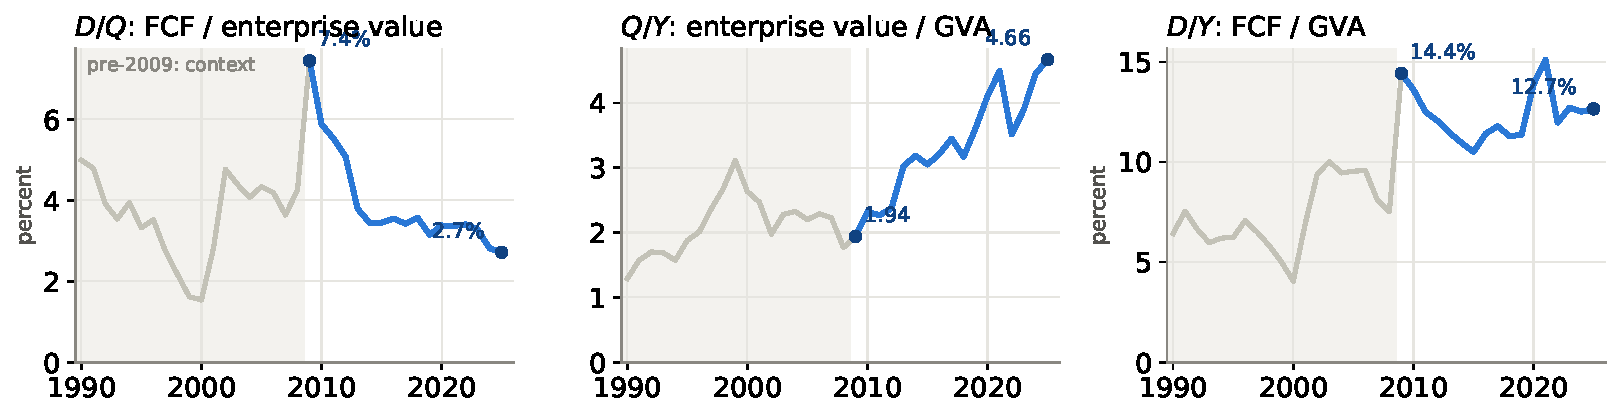
\includegraphics[width=0.9\textwidth]{figures/a_f_ratios.pdf}}
\vspace{0.05cm}
\begin{columns}[T]
\column{0.56\textwidth}
{\scriptsize\setlength{\tabcolsep}{3.5pt}
\begin{tabular}{@{}llrrrrr@{}}\toprule
 & Sector & 2009 & 2011 & 2025 & \multicolumn{2}{c}{$\Delta\log$ to 2025}\\
 & & & & & from 2009 & from 2011\\\midrule
$Q/Y$ & total corp. & \vc{rec_total_QY2009} & \vc{rec_total_QY2011} & \vc{rec_total_QY2025} & \vc{rec_total_dQY2009} & \vc{rec_total_dQY2011}\\
 & NFC & \vc{rec_nfc_QY2009} & \vc{rec_nfc_QY2011} & \vc{rec_nfc_QY2025} & \vc{rec_nfc_dQY2009} & \vc{rec_nfc_dQY2011}\\
$D/Y$, \% & total corp. & \vc{rec_total_DY2009} & \vc{rec_total_DY2011} & \vc{rec_total_DY2025} & \vc{rec_total_dDY2009} & \vc{rec_total_dDY2011}\\
 & NFC & \vc{rec_nfc_DY2009} & \vc{rec_nfc_DY2011} & \vc{rec_nfc_DY2025} & \vc{rec_nfc_dDY2009} & \vc{rec_nfc_dDY2011}\\
$D/Q$, \% & total corp. & \vc{rec_total_DQ2009} & \vc{rec_total_DQ2011} & \vc{rec_total_DQ2025} & & \\
 & NFC & \vc{rec_nfc_DQ2009} & \vc{rec_nfc_DQ2011} & \vc{rec_nfc_DQ2025} & & \\\bottomrule
\end{tabular}}
\column{0.41\textwidth}
{\scriptsize In both sectors $Q/Y$ about doubles from 2011 while $D/Y$ ends near its 2011 level: the fall in the yield is a rise in $Q$, not a fall in $D$. $Q/Y$ accounts for \vc{rec_total_shQY2009}\% (2009 base) and \vc{rec_total_shQY2011}\% (2011 base) of $\Delta\log(Q/D)$ in the total corporate sector, \vc{rec_nfc_shQY2009}\% and \vc{rec_nfc_shQY2011}\% in the NFC sector. NFC $D/Y$ drifts down slightly, so there the $D/Y$ term takes \vc{rec_nfc_shDY2011}--\vc{rec_nfc_shDY2009}\%. Part I uses total corporate, Part II NFC.\par}
\end{columns}
\src{Total corporate: Codes/Calibration\_R1/2\_Check/figures/figure\_data.csv (AHP mapping of Fed Z.1 and BEA IMA, nominal). NFC: Z.1 via FRED, $D=\mathrm{NOS}-T-\mathrm{NCF}$ (18 Nov deck, data/processed/z1\_nfc\_ratios\_pct\_gva.csv). $Y$ is each sector's own GVA.}
\end{frame}

% ================================================================ synthesis
\begin{frame}[label=fr-synth]{$Q/Y$ doubles; the ratio each mechanism needs to move does not}{Each ratio over its own sector's GVA, index 2011 $=100$; dashed: $Q/Y$ of the same sector}
\vspace{-0.2cm}
\centerline{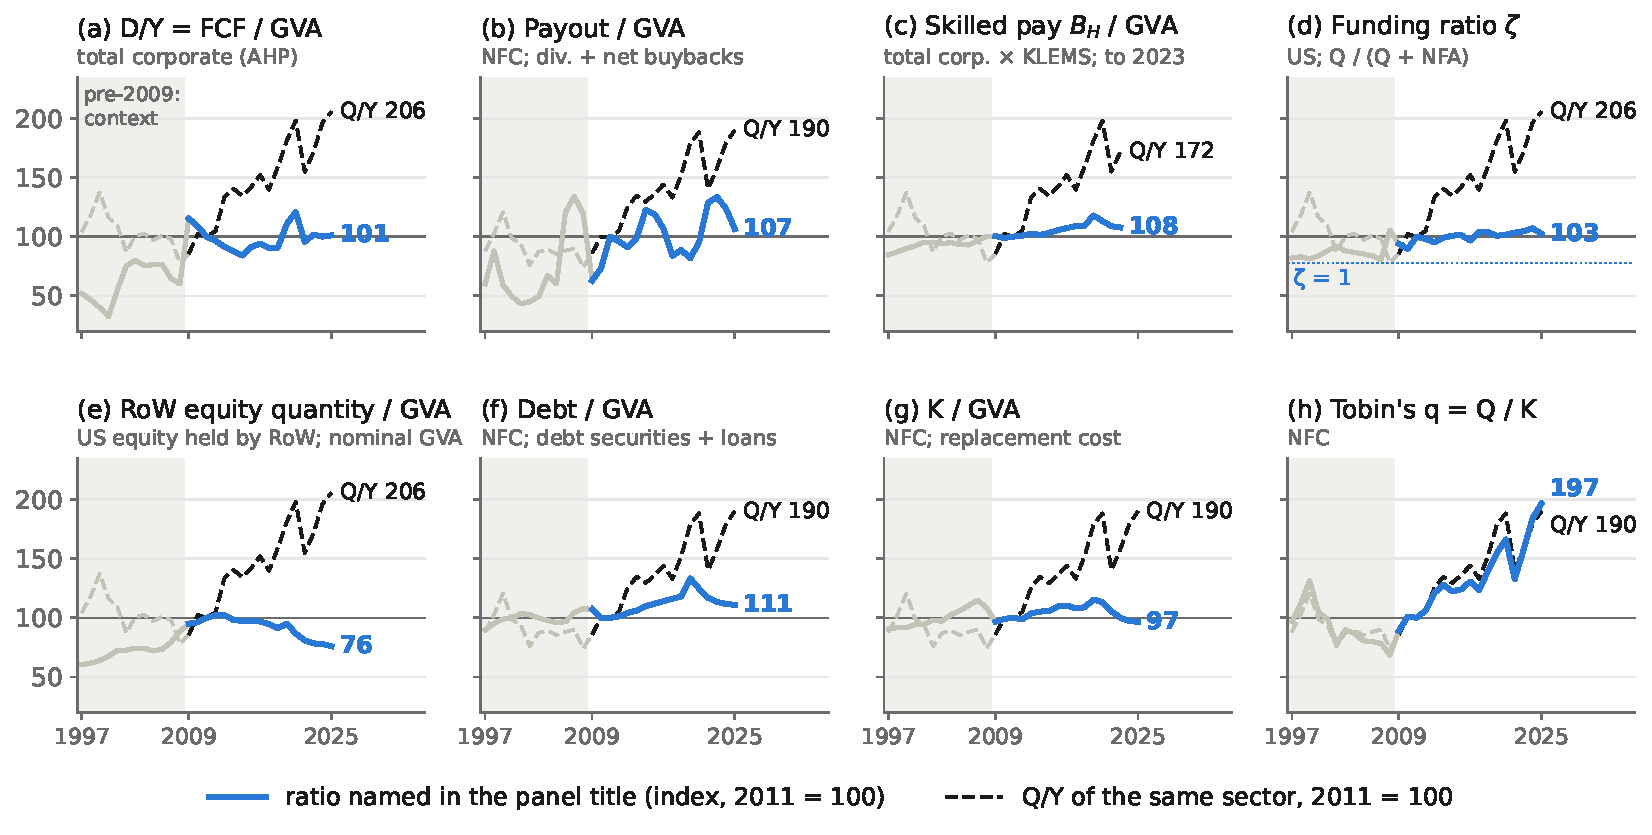
\includegraphics[width=0.8\textwidth]{figures/s_synthesis_indexed_ratios.pdf}}
\vspace{-0.05cm}
{\scriptsize Base 2011 because 2009 FCF is a crisis spike. On a 2009 base the 2025 values are: $D/Y$ \vc{idx09_DY}, payout \vc{idx09_PAY}, $B_H/Y$ \vc{idx09_BHY} (2023), $\zeta$ \vc{idx09_ZETA}, RoW equity quantity \vc{idx09_XQ}, Debt \vc{idx09_DEBT}, $K/Y$ \vc{idx09_KY}, $q$ \vc{idx09_q}; $Q/Y$ \vc{idx09_QY_total} (total corporate), \vc{idx09_QY_nfc} (NFC). Only $q$ tracks $Q/Y$.\par}
\src{(a), (c) figure\_data.csv, (c) with the KLEMS college share. (d) zeta\_funding\_ratio\_1990\_2025.csv (Sep 2026 release); dotted: $\zeta=1$. (e) AHP\_NFA (June 2026 release): quantity of US equity held by RoW = the position (foreign-held US equity) over its price index, divided by nominal corporate GVA. (b), (f)--(h) 18 Nov deck, z1\_nfc\_ratios\_pct\_gva.csv. Data: data/synthesis\_indexed\_ratios.csv.}
\end{frame}

% ================================================================ PART I
\begin{frame}[label=fr-hkt]{I. The HKT channel and what it predicts}{Model; tested on the US total corporate sector (AHP)}
\begin{columns}[T]
\column{0.53\textwidth}
\setlength{\abovedisplayskip}{2pt}\setlength{\belowdisplayskip}{2pt}\setlength{\abovedisplayshortskip}{1pt}\setlength{\belowdisplayshortskip}{1pt}
{\small Per-variety dividend and price under free entry, with $X_t\equiv\varphi_tH$ the skilled labor used in production:}
\[
d_t=\frac{1-\vartheta}{\vartheta}\,\frac{w_{H,t}\,\overbrace{\varphi_tH}^{X_t}}{N_t},\qquad q_t=\frac{w_{H,t}}{aN_t},
\]
\[
\frac{d_t}{q_t}=a\,\frac{1-\vartheta}{\vartheta}\,X_t .
\]
{\small Funding cap (two-period OLG): $\;Q_t+\mathrm{NFA}_t=\beta e_t$.}\\[0.05cm]
{\small Free entry and the knowledge law: $\;\Qc_t=N_{t+1}q_t=(G_t/a)\,w_{H,t}$.}\\[0.1cm]
{\small Unbalanced growth ($\rho>1$, $\xi_u>\nu_u$) pulls skilled labor out of production:}
\[
\varphi_t\to0\iff X_t\to0\;\Longrightarrow\; \frac{D_t}{Y_t}\to0,\;\; \frac{Q_t}{D_t}\to\infty .
\]
\column{0.43\textwidth}
\begin{block}{Testable predictions ($u$ regime)}
\small
\begin{enumerate}\setlength{\itemsep}{0.08cm}
\item $Q$ is capped by $\beta e$, so a rising $Q/D$ must come from \textbf{$D/Y$ (equivalently $D/e$) falling}, not from $Q/Y$ rising (slides \ref{fr-decomp}--\ref{fr-payout}).
\item Free entry gives $B_H/Q=aH/G$: with constant $a$ and $G\approx1$, \textbf{$B_H/Q$ rises with $H$} (\slref{fr-free}).
\item The funding ratio $\zeta_t=Q_t/(Q_t+\mathrm{NFA}_t)$ tends to 1 in the tail (\slref{fr-zeta}).
\end{enumerate}
\end{block}
\vspace{0.05cm}
{\scriptsize Model and data are compared on which term drives the fall in $D/Q$, on sign and direction, not on levels at a date.\par}
\end{columns}
\src{Equations from AI\_drafting/V6\_production.tex (dividend yield, free entry, funding identity). $q_t$ here is the price of one variety, not Tobin's $q$ of Part II.}
\end{frame}

\begin{frame}[label=fr-decomp]{I(a). Decomposition: the model gets the channel backwards}{Data (US total corporate sector, AHP) vs model, and how AHP read the same data}
\begin{columns}[T]
\column{0.5\textwidth}
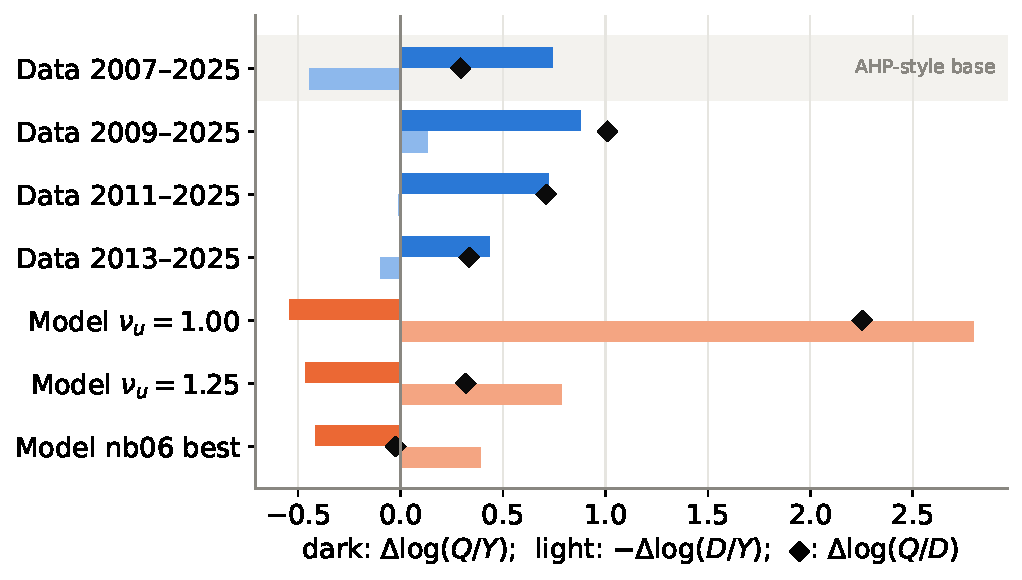
\includegraphics[width=\linewidth]{figures/a_f_decomposition.pdf}\\[0.05cm]
{\scriptsize\setlength{\tabcolsep}{3pt}
\begin{tabular}{@{}lrcrcr@{}}\toprule
 & $\Delta\log\frac{Q}{D}$ & $=$ & $\Delta\log\frac{Q}{Y}$ & $-$ & $\Delta\log\frac{D}{Y}$\\\midrule
Data 2007--25 & \va{dQD2007} & & \va{dQY2007} & & \va{dDY2007}\\
Data 2009--25 & \va{dQD2009} & & \va{dQY2009} & & \va{dDY2009}\\
Data 2011--25 & \va{dQD2011} & & \va{dQY2011} & & \va{dDY2011}\\
Model $\nu_u=1$, $t=1$--80 & 2.25 & & \va{mQY100} & & \va{mDY100}\\\bottomrule
\end{tabular}}
\column{0.47\textwidth}
{\footnotesize
\textbf{Model.} $D/Q$ falls because $D/Y$ collapses (1.39\% to 0.08\% for $\nu_u=1$); $Q/Y$ even falls. All three simulated paths look like this.\\[0.15cm]
\textbf{Data from 2009.} $Q/Y$ accounts for \va{shQY2009}\% (2009 base) to \va{shQY2011}\% (2011 base) of $\Delta\log(Q/D)$; $D/Y$ is flat.\\[0.15cm]
\textbf{AHP.} FCF/EV is roughly stable over the last decade relative to pre-2007, so they attribute the rise in $Q/Y$ to the rise in FCF/$Y$. On a 2007 base, $D/Y$ does account for \va{shDYofQY2007}\% of $\Delta\log(Q/Y)$; on a 2009 or 2011 base, \va{shDYofQY2009}\% and \va{shDYofQY2011}\%.\\[0.15cm]
\textcolor{inksec}{The contrast with AHP is a base-year contrast: $D/Y$ jumps between 2007 and 2009 and is flat inside the $u$-regime window.}}
\end{columns}
\src{Model: Two\_country\_proudction\_zero\_nu\_b, notebooks 05--06 (AHP-seeded calibration), $t=1$--80 for $\nu_u\in\{1,1.25\}$, $t=1$--16 for the nb06 best point. AHP: The End of Privilege, Section 2, Figures 8--9. Data: figure\_data.csv.}
\end{frame}

\begin{frame}[label=fr-payout]{I(b). Payout form: buybacks are already in $D$, and payout$/Y$ rises}{Figure: Compustat US nonfinancial firms. Table: NFC (Z.1), $D$ = FCF or shareholder payout}
\centerline{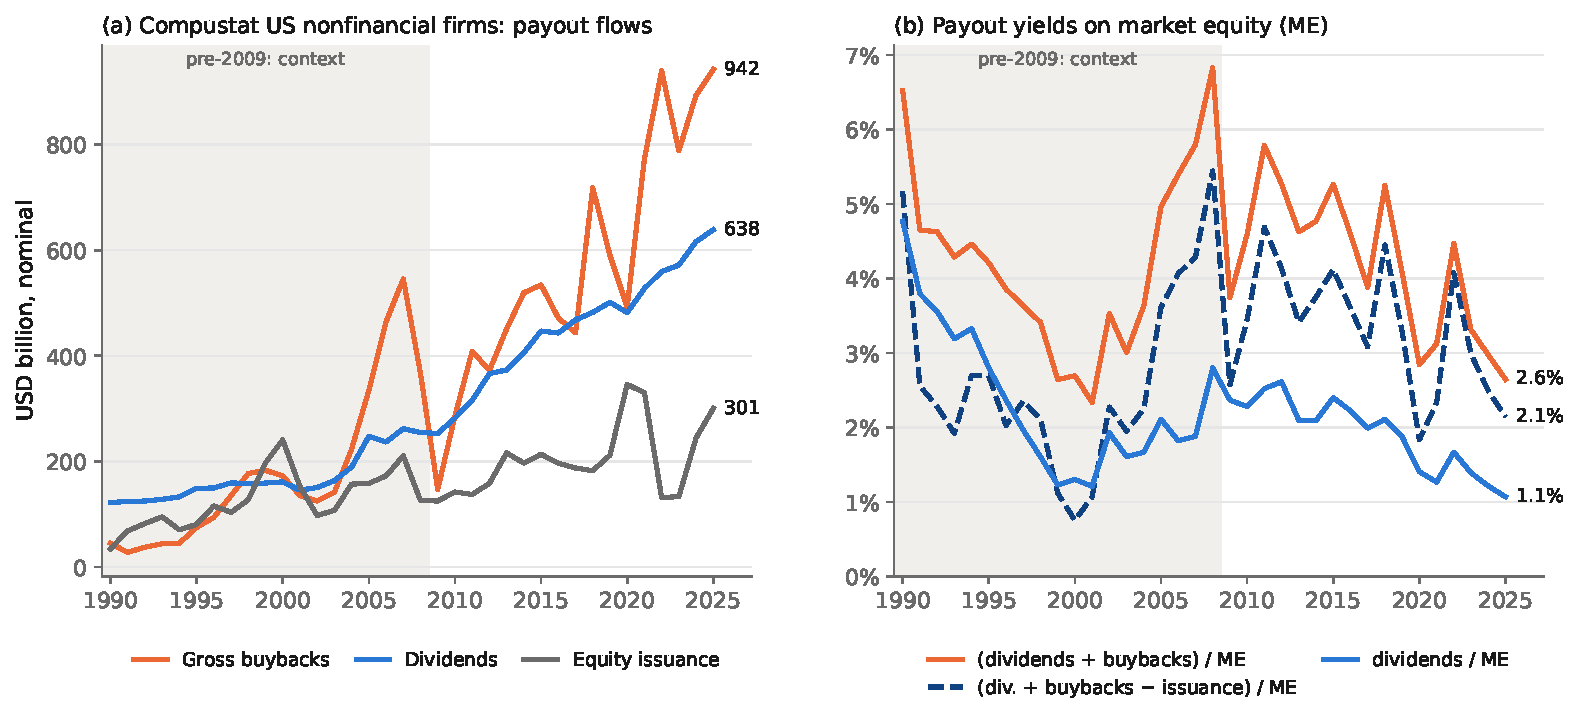
\includegraphics[height=0.43\textheight]{figures/b_f4_compustat_payout.pdf}}
\vspace{-0.15cm}
\begin{columns}[T]
\column{0.56\textwidth}
{\scriptsize\setlength{\tabcolsep}{3.5pt}
\begin{tabular}{@{}llrrrr@{}}\toprule
Base & $D/Q$, NFC (Z.1) & start & 2025 & $\Delta\log\frac{Q}{Y}$ & $\Delta\log\frac{D}{Y}$\\\midrule
2009 & FCF / $Q$ & \vb{rob_fcfa_yield_start}\% & \vb{rob_fcfa_yield_end}\% & $\vb{rob_fcfa_dlog_QY}$ & $\vb{rob_fcfa_dlog_DY}$\\
 & payout / equity & \vb{rob_deqa_yield_start}\% & \vb{rob_deqa_yield_end}\% & $\vb{rob_deqa_dlog_QY}$ & $\vb{rob_deqa_dlog_DY}$\\
2011 & FCF / $Q$ & \vb{rob_fcfb_yield_start}\% & \vb{rob_fcfb_yield_end}\% & $\vb{rob_fcfb_dlog_QY}$ & $\vb{rob_fcfb_dlog_DY}$\\
 & payout / equity & \vb{rob_deqb_yield_start}\% & \vb{rob_deqb_yield_end}\% & $\vb{rob_deqb_dlog_QY}$ & $\vb{rob_deqb_dlog_DY}$\\
3-yr avg & FCF / $Q$ & \vb{rob_fcfc_yield_start}\% & \vb{rob_fcfc_yield_end}\% & $\vb{rob_fcfc_dlog_QY}$ & $\vb{rob_fcfc_dlog_DY}$\\
 & payout / equity & \vb{rob_deqc_yield_start}\% & \vb{rob_deqc_yield_end}\% & $\vb{rob_deqc_dlog_QY}$ & $\vb{rob_deqc_dlog_DY}$\\\bottomrule
\end{tabular}}
\column{0.4\textwidth}
{\scriptsize $D=$ FCF is measured before financing, so dividends vs buybacks does not change it. With $D$ = net dividends + net buybacks, $D/Y$ rises (NFC: \vb{DEQY2009}\% in 2009, \vb{DEQY2011}\% in 2011, \vb{DEQY2025}\% in 2025); the payout yield falls only because equity value rises. Compustat 2009--25: buybacks \$\vb{cs_cumbuy} tn, dividends \$\vb{cs_cumdiv} tn, issuance \$\vb{cs_cumiss} tn. Market equity $\times$\vb{cs_me_mult}, gross payout $\times$\vb{cs_pay_mult} (2011 base: $\times$\vb{cs_me_multB} vs $\times$\vb{cs_pay_multB}).\par}
\end{columns}
\src{Payout = net dividends + net buybacks; equity = $E+\mathrm{FDI}^{mv}$. 3-yr avg: 2009--11 vs 2023--25. Compustat funda, fic = USA, SIC outside 6000--6999; ME = csho$\times$prcc\_f. Worked example of why FCF does not depend on the payout form: \slref{xcash}.}
\end{frame}

\begin{frame}[label=fr-gva]{I(c). Skilled labor (1): the growing parts of GVA}{US total corporate GVA (AHP), percent; compensation split with the BEA--BLS KLEMS college share}
\centerline{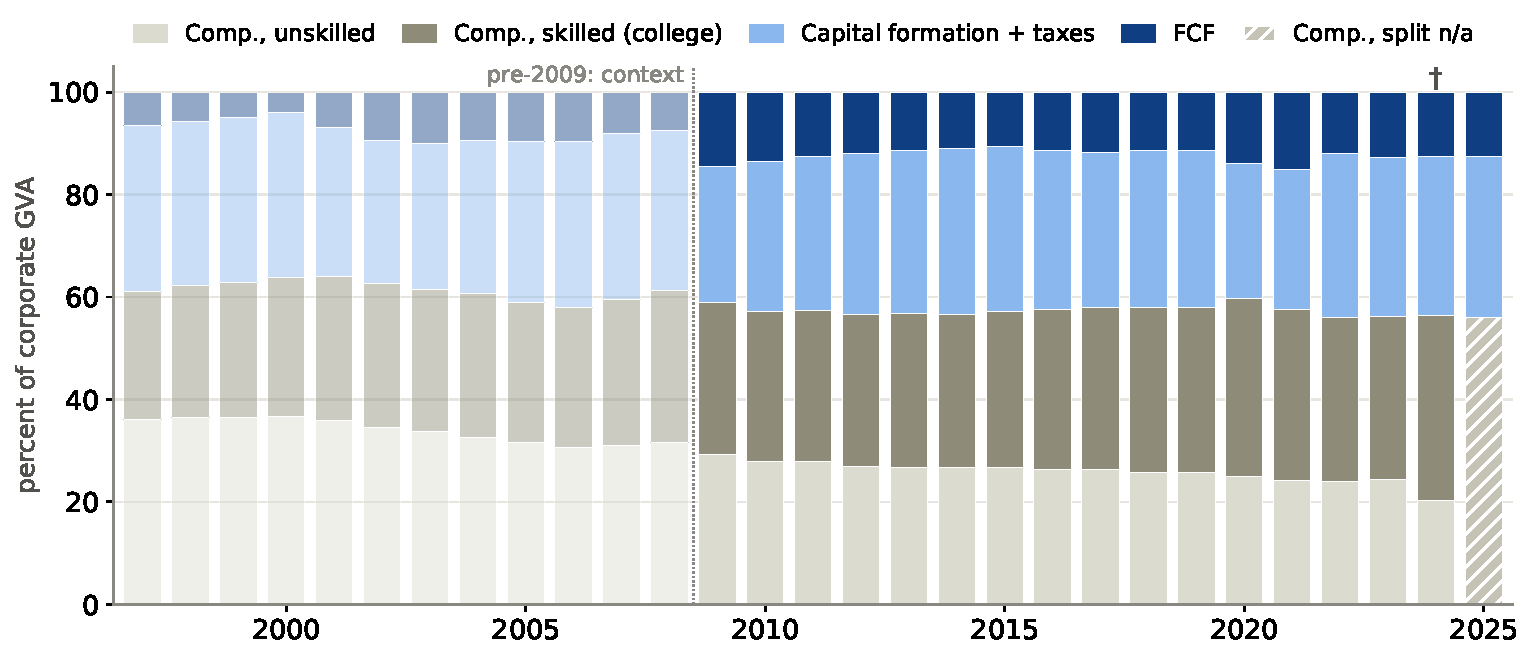
\includegraphics[width=0.74\textwidth]{figures/a_f_gva_percent.pdf}}
\vspace{0.0cm}
{\scriptsize Since 2009 two shares rise: skilled compensation (\va{g_skilled_sh2009}\% to \va{g_skilled_sh2023}\% in 2023) and capital formation and taxes (\va{g_kap_sh2009}\% to \va{g_kap_sh2023}\%). Unskilled compensation (\va{g_unskilled_sh2009}\% to \va{g_unskilled_sh2023}\%) and FCF (\va{g_fcf_sh2009}\% to \va{g_fcf_sh2023}\%) fall. Of the $+$\va{Y_dtn} tn rise in GVA over 2009--23, capital formation and taxes take \va{g_kap_contrib}\%, skilled compensation \va{g_skilled_contrib}\%, unskilled \va{g_unskilled_contrib}\%, FCF \va{g_fcf_contrib}\%. KLEMS skilled share of compensation: \va{ss_klems2009}\% to \va{ss_klems2023}\% (ACS bridge \va{ss_acs2009}\% to \va{ss_acs2023}\%, CPS bridge \va{ss_cps2009}\% to \va{ss_cps2023}\%).\par}
\src{Capital formation and taxes $=Y-\mathrm{COMP}-\mathrm{FCF}$. \dag\ 2024: likely KLEMS source break; 2025: no KLEMS split yet. Pre-2009 faded. Trillion USD and the full contributions table, with why KLEMS rather than CPS or ACS: slides \ref{fr-gvatn}--\ref{fr-contrib}.}
\end{frame}

\begin{frame}[label=fr-labor]{I(c). Skilled labor (2): employment and wages grow; the premium is flat}{BEA--BLS production account, private industries}
\begin{columns}[T]
\column{0.57\textwidth}
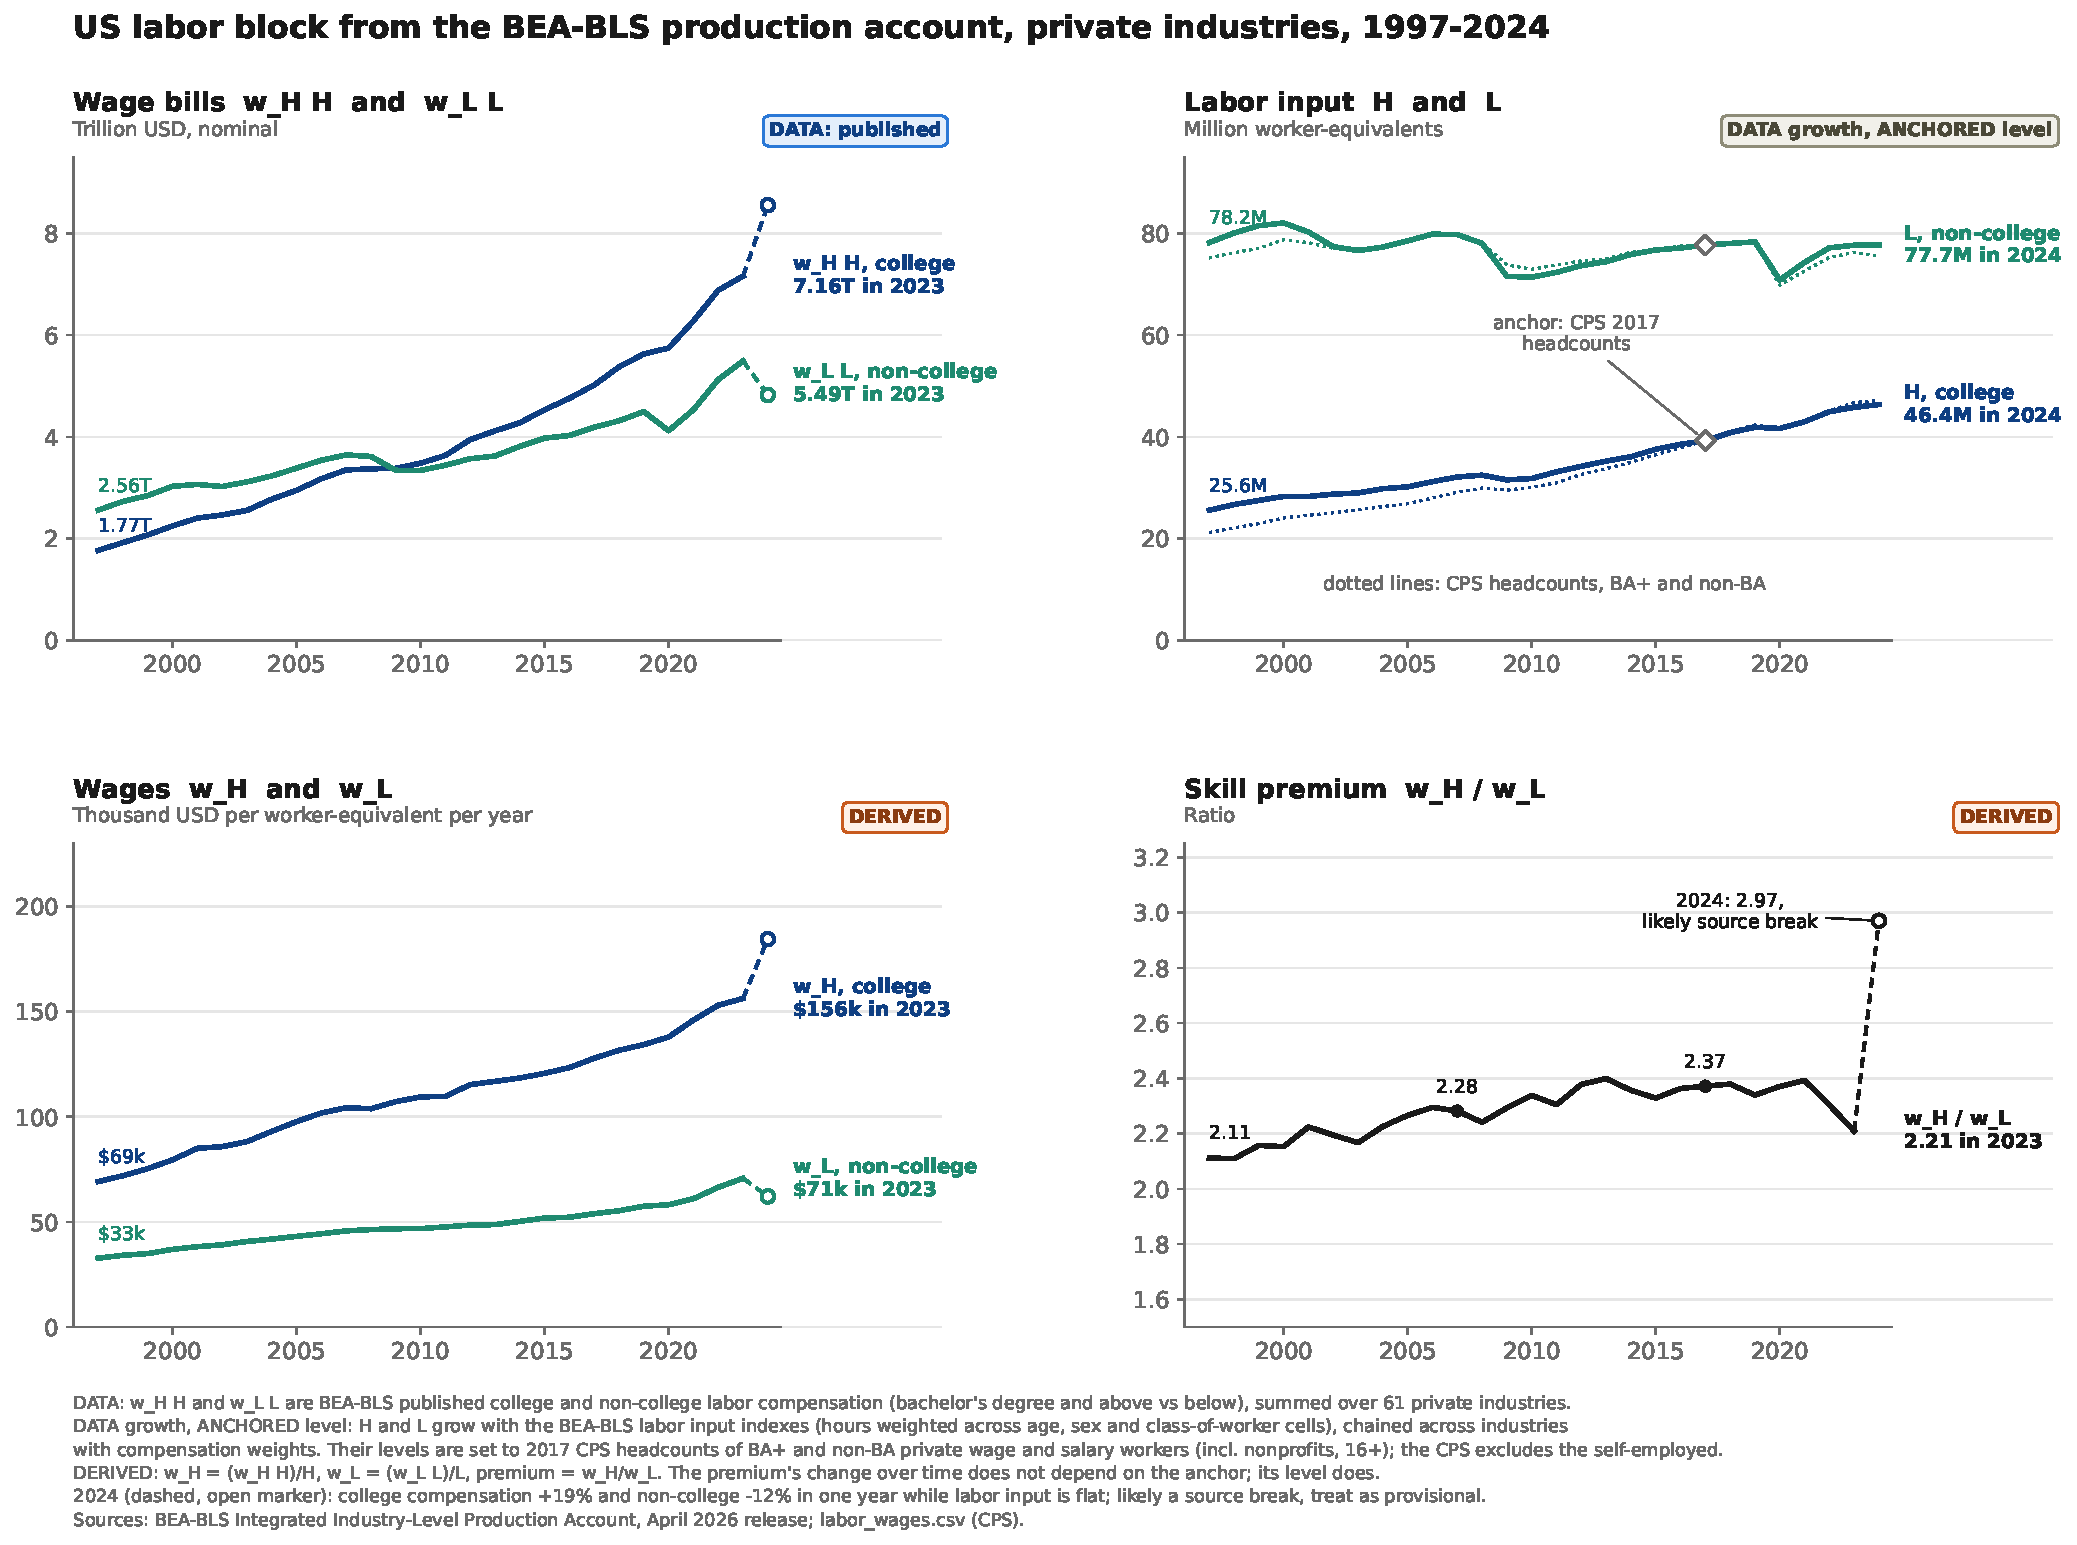
\includegraphics[width=\linewidth]{figures/a_c_labor_klems.pdf}
\column{0.41\textwidth}
{\footnotesize
\begin{tabular}{@{}lrr@{}}\toprule
2009$\to$2023 & multiple & per year\\\midrule
$H$ & $\times$\va{k_H_mult} & \va{k_H_gr}\%\\
$L$ & $\times$\va{k_L_mult} & \va{k_L_gr}\%\\
\con{$w_H$} & $\times$\va{k_wH_mult} & \va{k_wH_gr}\%\\
\con{$w_L$} & $\times$\va{k_wL_mult} & \va{k_wL_gr}\%\\
$B_H=w_HH$ & $\times$\va{k_BH_mult} & \va{k_BH_gr}\%\\
$B_L=w_LL$ & $\times$\va{k_BL_mult} & \va{k_BL_gr}\%\\\bottomrule
\end{tabular}}\\[0.2cm]
{\scriptsize Skilled employment and the skilled wage both grow steadily ($w_H$: \$\va{k_wH2009}k to \$\va{k_wH2023}k), so the skilled wage bill doubles. The gap between $B_H$ and $B_L$ is quantity: $w_L$ grows as fast as $w_H$; the \con{premium} is flat (\va{k_prem2009} in 2009, \va{k_prem2023} in 2023).}\\[0.1cm]
{\scriptsize\textcolor{inksec}{The 2023--24 jump in the CPS skill premium is a Census top-code change (slides \ref{fr-topcode}--\ref{fr-premium}).}}
\end{columns}
\src{$w_HH$, $w_LL$: published. $H$, $L$: KLEMS labor-input growth, levels anchored to 2017 CPS headcounts. $w_H$, $w_L$, premium: derived. The 2024 KLEMS split is treated as a break.}
\end{frame}

\begin{frame}[label=fr-free]{I(c). Skilled labor (3): free entry needs $B_H/Q$ to rise with $H$; it falls}{$Q$, $B_H$: US total corporate sector (AHP) with the KLEMS college share; $H$: KLEMS college labor input}
\centerline{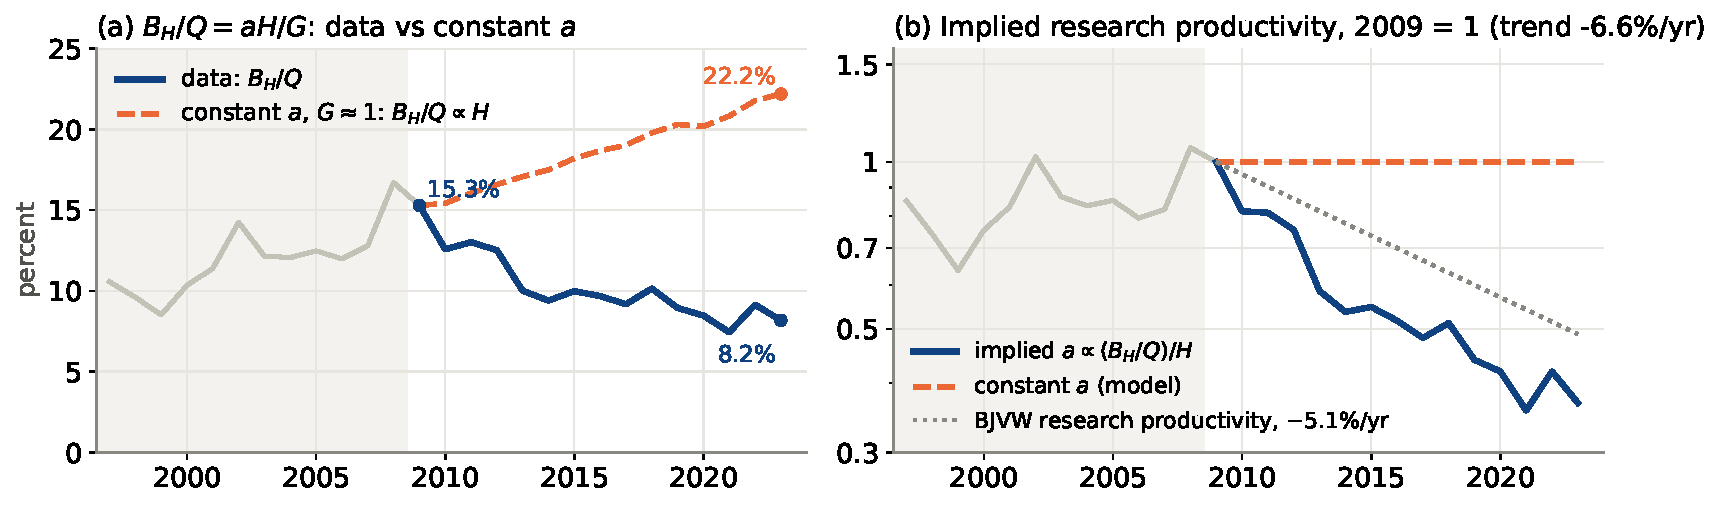
\includegraphics[width=0.95\textwidth]{figures/a_f_free_entry.pdf}}
\vspace{0.05cm}
{\small Free entry and the knowledge law give $\Qc_t=N_{t+1}q_t=(G_t/a)\,w_{H,t}$, so $B_H/Q=aH/G$. With constant $a$ and $G\approx1$, $B_H/Q$ should grow with $H$ ($\times$\va{feHmult}, 2009--23), reaching \va{feBHQcf2023} in 2023 (dashed). The data fall from \va{feBHQ2009} to \va{feBHQ2023}. Implied \imp{$a$}: \va{feaSlope}\%/yr, against BJVW's $-5.1$\%/yr. Skilled pay rises with GVA (\slref{fr-gva}); $Q$ rises faster.}
\src{$B_H$: corporate compensation $\times$ KLEMS college share; $H$: KLEMS college labor input (2017 CPS anchor); ends 2023. CPS bridge: same pattern. $Q$ is enterprise value and includes installed capital (\slref{fr-corpcap}).}
\end{frame}

\begin{frame}[label=fr-zeta]{I(d). Funding side: $\zeta$ stays well above the theory's limit of one}{US: $Q$ = AHP total-corporate enterprise value, NFA from the AHP external accounts}
\centerline{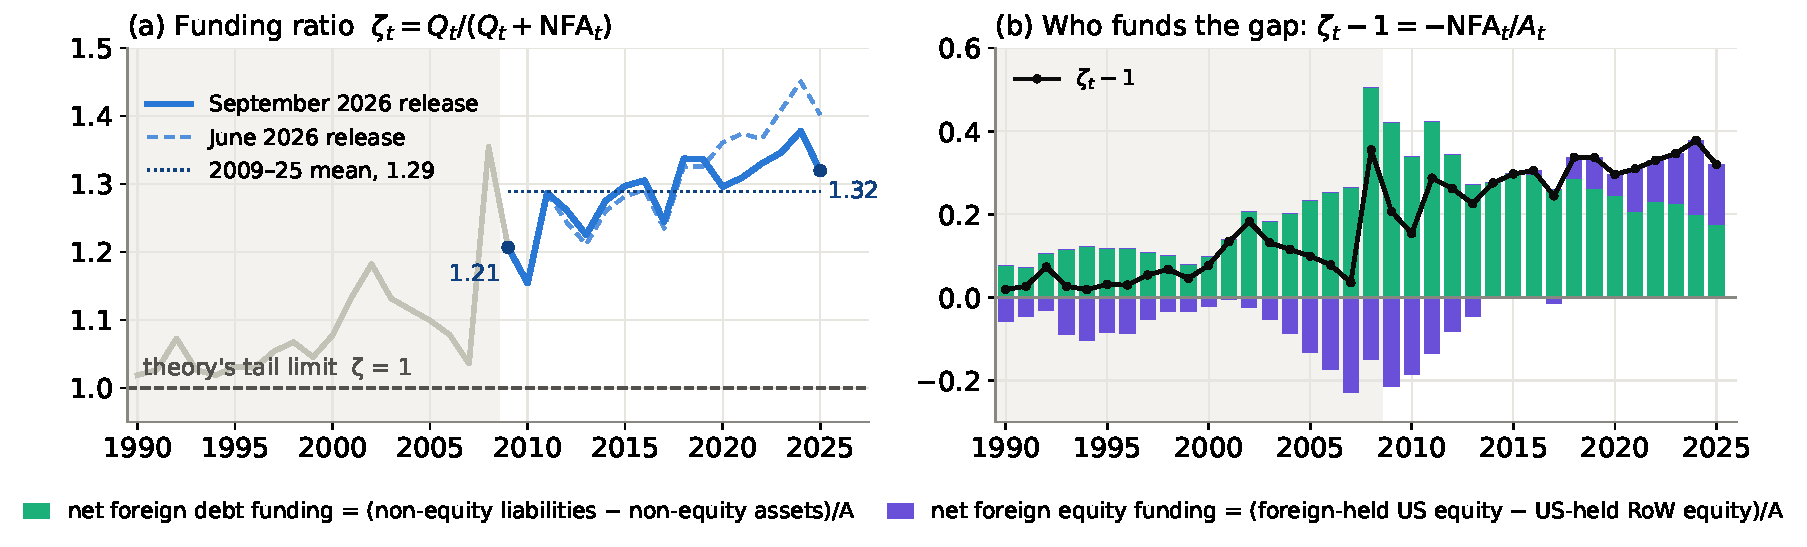
\includegraphics[width=0.88\textwidth]{figures/a_f_zeta.pdf}}
\vspace{0.05cm}
\begin{columns}[T]
\column{0.44\textwidth}
{\footnotesize $A_t=\beta e_t$ and zero-net-supply bonds give $\mathrm{NFA}_t=A_t-Q_t$, so
\[
\con{\zeta_t}=\frac{Q_t}{\beta e_t}=\frac{Q_t}{Q_t+\mathrm{NFA}_t}=1-\frac{\mathrm{NFA}_t}{A_t},
\]
with no $\beta$ and no income series.}
\column{0.52\textwidth}
{\footnotesize The HKT tail needs $\zeta_t\to1$. In the data $\zeta>1$ in every year since 1990 (minimum \va{zmin_all}): \va{z2009} (2009), \va{z2011} (2011), \va{z2025} (2025; \va{zjun2025} on the June release); 2009--25 mean \va{zmean}, trend +\va{zslope}\,pp per year. Since 2009 net foreign funding has moved from debt to equity, with its total about unchanged.}
\end{columns}
\src{Codes/Calibration\_R1/2\_Check/figures/zeta\_funding\_ratio\_1990\_2025.csv; September 2026 release, June-consistent line for comparison; $Q$ and NFA always from one release.}
\end{frame}

\begin{frame}[label=fr-ext]{I(e). The external side of the repricing is valuation, not purchases}{Foreign-held US equity (portfolio + FDI, market value), AHP external accounts}
\centerline{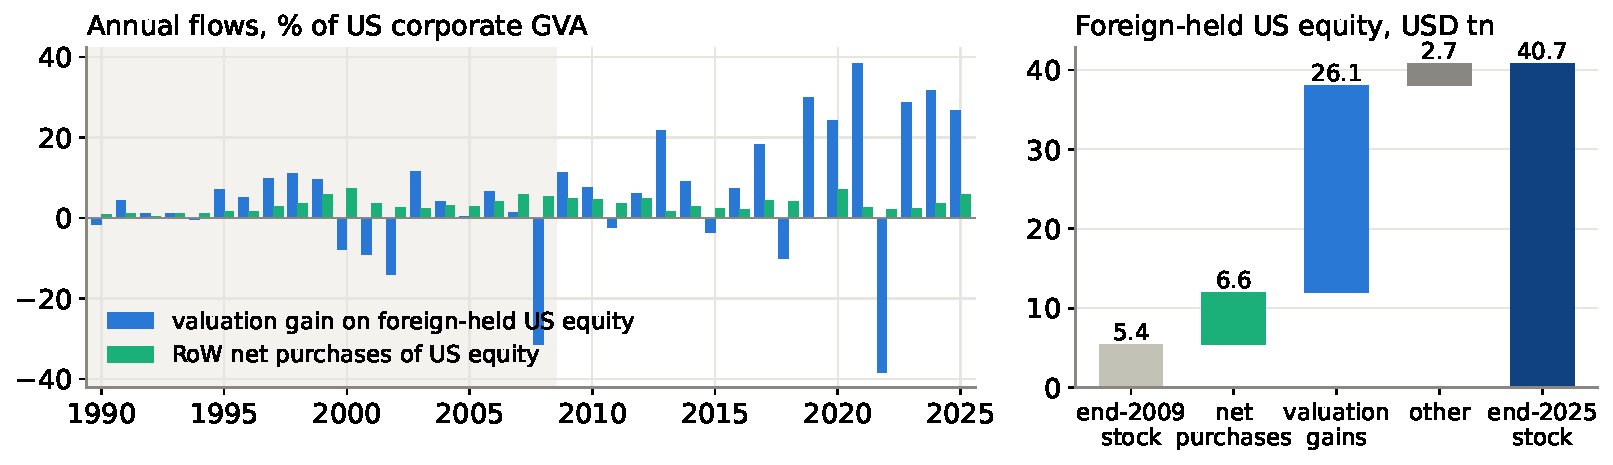
\includegraphics[width=0.88\textwidth]{figures/a_f_valuation.pdf}}
\vspace{0.05cm}
\begin{columns}[T]
\column{0.5\textwidth}
{\footnotesize\setlength{\tabcolsep}{4pt}
\begin{tabular}{@{}lrr@{}}\toprule
\% of corporate GVA per year & 2002--07 & 2009--25\\\midrule
RoW net purchases of US equity & \va{x_purch_pre} & \va{x_purch_post}\\
Valuation gains, foreign-held & \va{x_gain_pre} & \va{x_gain_post}\\\bottomrule
\end{tabular}}\\[0.1cm]
{\footnotesize End-2009 to end-2025: \va{x_EL2009} to \va{x_EL2025} tn USD; purchases \va{x_purch_sh2009}\%, valuation \va{x_gain_sh2009}\%, other \va{x_other_sh2009}\% (2011 base: \va{x_purch_sh2011}/\va{x_gain_sh2011}/\va{x_other_sh2011}).}
\column{0.46\textwidth}
{\footnotesize Price of foreign-held US equity $\times$\va{x_pL} vs $\times$\va{x_pA} for US-held RoW equity; RoW's quantity $\times$\va{x_qtyL}, below GVA ($\times$\va{x_gva}).\\[0.1cm]
The rise in $Q/Y$ is a common repricing of US equity. RoW's large gross position transmits it to the NFA, as in AHP; RoW does not buy more.}
\end{columns}
\src{Empirical\_Data/AHP\_NFA/ahp\_us\_nfa\_decomposition\_latest.csv (June 2026 release); annual sums of quarterly flows over mean SAAR corporate GVA.}
\end{frame}

% ================================================================ PART II
\begin{frame}[label=fr-acct]{II. Accounting: where credit, capital and buybacks enter}{NFC sector (Z.1); the detailed version of the identities on \slref{fr-framework}}
\begin{columns}[T]
\column{0.58\textwidth}
{\small\textbf{Value side} (Fed series FL102010405, the AHP $Q$):}
{\footnotesize\[
Q=\underbrace{E+\mathrm{FDI}^{mv}}_{\text{equity at market value}}+\underbrace{\mathrm{Debt}}_{\text{securities + loans}}+\underbrace{(\mathrm{OL}-\mathrm{FA})}_{\text{other liab.} - \text{fin. assets}}
\]}
{\small\textbf{Capital side}, with $K$ = nonfinancial assets at replacement cost:}
{\footnotesize\[
\frac{Q}{Y}=\underbrace{\frac{Q}{K}}_{\text{Tobin's }q}\times\frac{K}{Y}
\]}
{\small\textbf{Cash-flow side} (Z.1 S.5.a, exact; drawn on \slref{fr-fcf}):}
{\scriptsize\begin{align*}
\underbrace{\mathrm{NOS}-T-\mathrm{NCF}}_{D=\mathrm{FCF}}&=\underbrace{\mathrm{Div}+\mathrm{BB}}_{\text{to shareholders}}+\underbrace{\mathrm{Int}-\Delta\mathrm{Debt}}_{\text{to creditors}}\\[-0.1cm]
&\quad+\underbrace{\mathrm{NAFA}-\Delta\mathrm{OL}-\mathrm{RE}}_{\text{net fin.\ saving}}+\underbrace{\mathrm{Rent}+\mathrm{Tr}+\mathrm{KT}+\mathrm{SD}}_{\text{other}}
\end{align*}}
\column{0.38\textwidth}
\begin{block}{What each channel can do}
\small
\begin{itemize}\setlength{\itemsep}{0.08cm}
\item A debt-financed buyback swaps $E$ for Debt: $Q$ and FCF unchanged.
\item Debt-financed investment raises $K$; $Q$ rises by $q\,\Delta K$ and FCF falls by NCF.
\item $Q/Y$ can rise with $D/Y$ flat only through $K/Y$ (capital deepening) or $q$ (valuation).
\end{itemize}
\end{block}
\vspace{0.12cm}
{\scriptsize So the question splits into: does $\mathrm{Debt}/Y$ or $K/Y$ rise, and does the payout form change $D$ (\slref{fr-payout})? \textcolor{inksec}{New to these data: slides \ref{xvalue}--\ref{xlink} explain both sides.}\par}
\end{columns}
\src{Fed Z.1 series analyzer: FL102010405 = FL103164105 + FL103192105 + FL104190005 $-$ FL104090005. Holds exactly in the downloaded data; same vintage as the project mapping file (max difference \vb{vintage_q_diff}\%).}
\end{frame}

\begin{frame}[label=fr-credit]{II(f). Credit: debt is flat relative to GVA; equity carries the rise in $Q/Y$}{NFC sector (Z.1), end-year stocks over annual NFC GVA}
\centerline{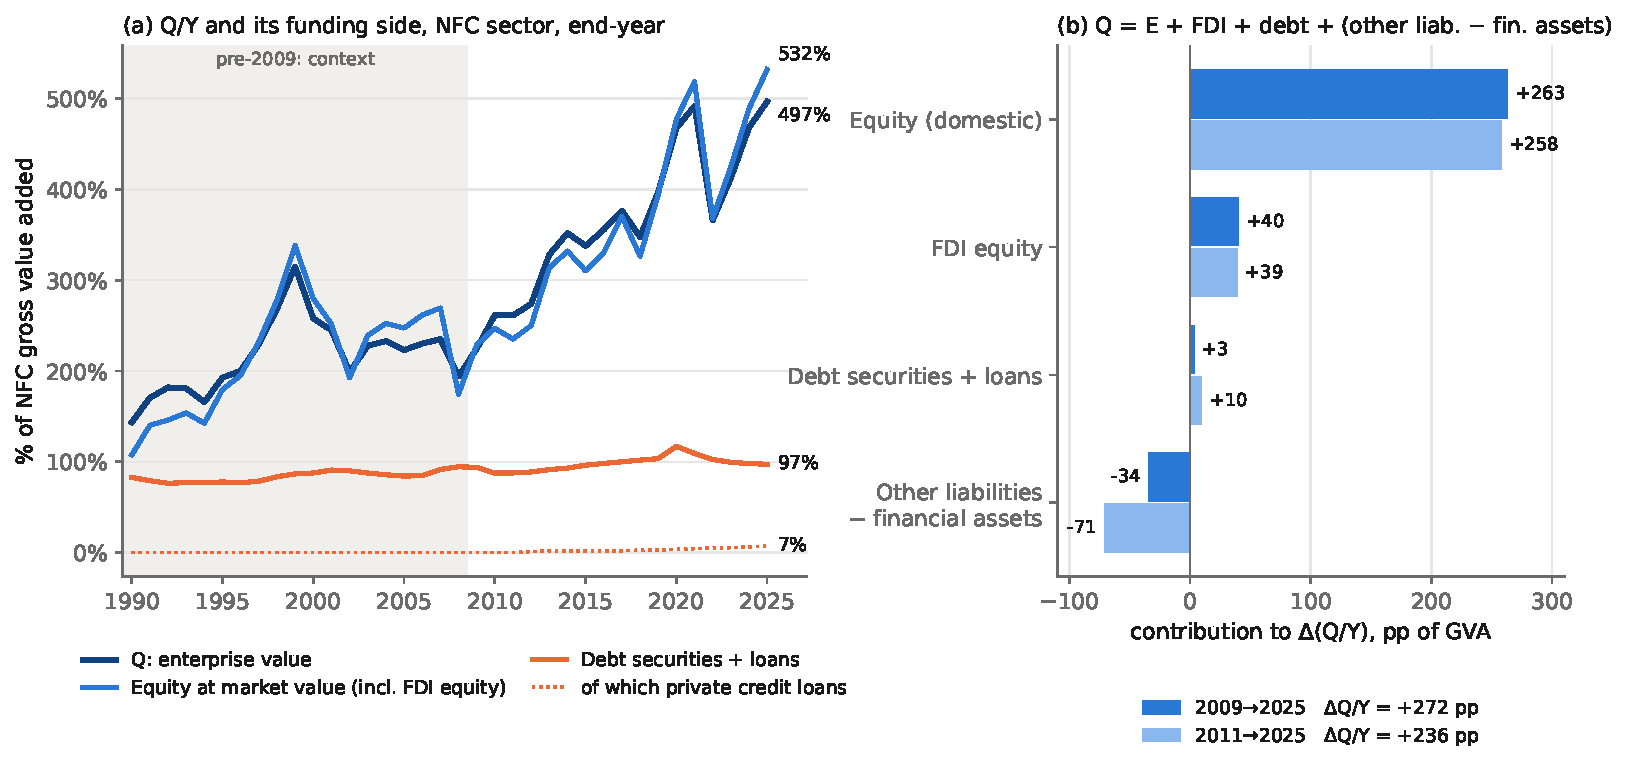
\includegraphics[height=0.45\textheight]{figures/b_f1_credit_q_funding.pdf}}
\vspace{-0.1cm}
{\scriptsize\setlength{\tabcolsep}{4pt}
\begin{tabular}{@{}lrrrrrr@{}}\toprule
\% of NFC GVA & 2007 & 2009 & 2011 & 2019 & 2025 & \vb{latest_q}\\\midrule
Debt securities + loans & \vb{DEBTY2007} & \vb{DEBTY2009} & \vb{DEBTY2011} & \vb{DEBTY2019} & \vb{DEBTY2025} & \vb{lat_DEBTY}\\
\quad bonds / loans & \vb{BONDSY2007} / \vb{LOANSY2007} & \vb{BONDSY2009} / \vb{LOANSY2009} & \vb{BONDSY2011} / \vb{LOANSY2011} & \vb{BONDSY2019} / \vb{LOANSY2019} & \vb{BONDSY2025} / \vb{LOANSY2025} & \\
\quad private-credit loans & -- & -- & -- & \vb{PCY2019} & \vb{PCY2025} & \vb{lat_PCY}\\
$Q$ & \vb{QY2007} & \vb{QY2009} & \vb{QY2011} & \vb{QY2019} & \vb{QY2025} & \vb{lat_QY}\\\bottomrule
\end{tabular}}\\[0.08cm]
{\scriptsize 2009--25: debt adds $+$\vb{dec2009_dDEBTY_pp} pp of the $+$\vb{dec2009_dQY_pp} pp rise in $Q/Y$; equity at market value $+$\vb{dec2009_dEY_pp} pp, FDI equity $+$\vb{dec2009_dFDIY_pp} pp. Debt/GVA ranges \vb{debt_min_post}--\vb{debt_max_post}\% over 2009--25.\par}
\src{Z.1 B.103/L.103 via FRED (BCNSDODNS, NCBDBIQ027S, BOGZ1FL103167205Q, NCBEILQ027S, BOGZ1LM103192105Q, TLBSNNCB, TFAABSNNCB, BOGZ1LM102010405Q); GVA BOGZ1FU106902501Q. \vb{latest_q}: stocks at end-quarter over trailing four-quarter GVA. Here $Q/Y$ is in \% of GVA (\slref{fr-fact} shows it as a ratio).}
\end{frame}

\begin{frame}[label=fr-capital]{II(g). Capital: $K/Y$ is flat; the rise in $Q/Y$ is a rise in Tobin's $q$}{NFC sector (Z.1); nonfinancial assets at replacement cost (real estate at market value)}
\centerline{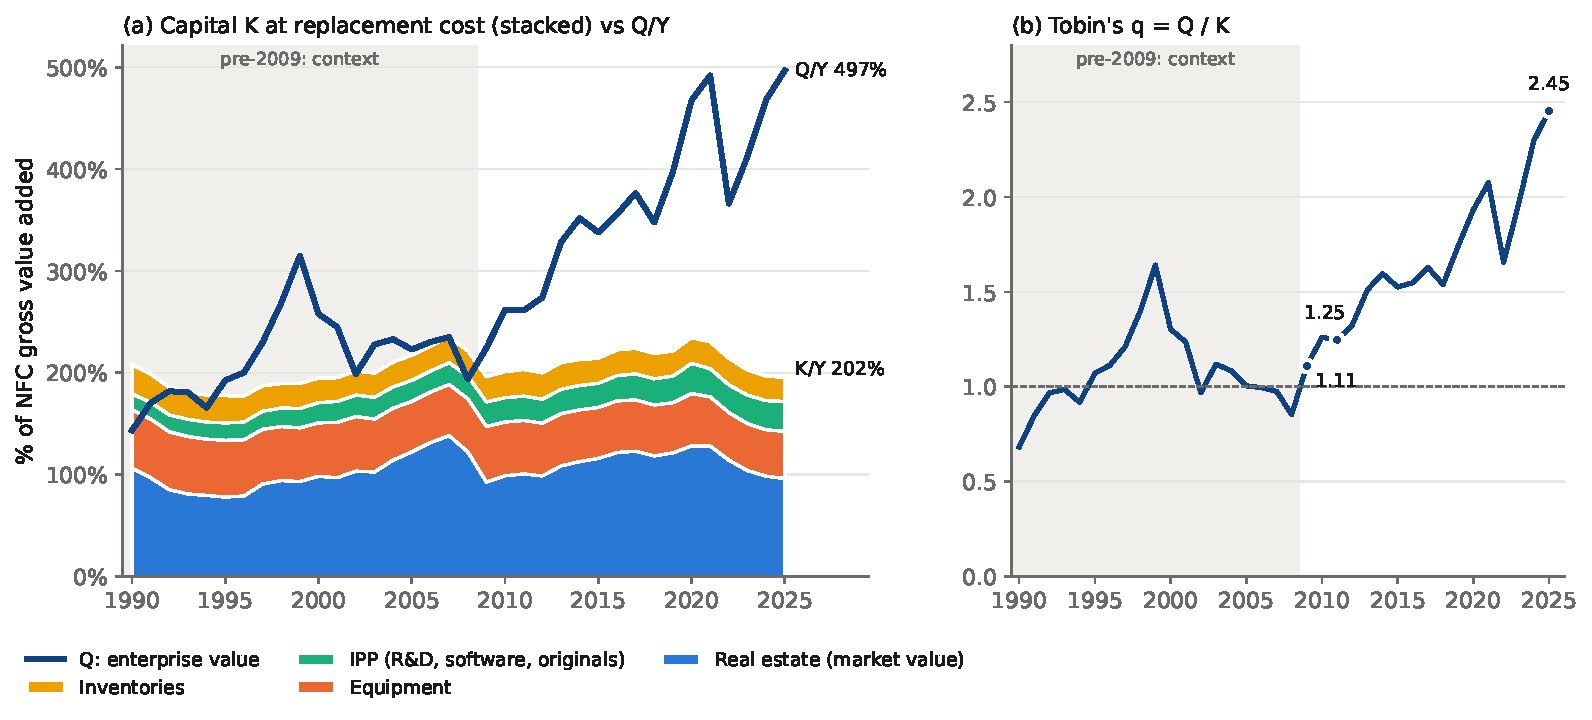
\includegraphics[height=0.47\textheight]{figures/b_f2_capital_tobin_q.pdf}}
\vspace{-0.1cm}
\begin{columns}[T]
\column{0.5\textwidth}
{\scriptsize\setlength{\tabcolsep}{4pt}
\begin{tabular}{@{}lrrrr@{}}\toprule
 & $\Delta\log\frac{Q}{Y}$ & $=\Delta\log q$ & $+\Delta\log\frac{K}{Y}$ & $q$ share\\\midrule
2009--25 & $\vb{dec2009_dlogQY}$ & $\vb{dec2009_dlog_q}$ & $\vb{dec2009_dlog_KY}$ & \vb{dec2009_sh_q}\%\\
2011--25 & $\vb{dec2011_dlogQY}$ & $\vb{dec2011_dlog_q}$ & $\vb{dec2011_dlog_KY}$ & \vb{dec2011_sh_q}\%\\\bottomrule
\end{tabular}}
\column{0.46\textwidth}
{\scriptsize Inside $K$, IPP (R\&D, software) rises from \vb{IPPY2009}\% to \vb{IPPY2025}\% of GVA and equipment falls from \vb{EQPY2009}\% to \vb{EQPY2025}\%; real estate is \vb{REY2009}\% in 2009 and \vb{REY2025}\% in 2025, after \vb{REY2007}\% at the 2007 peak. $K$ excludes intangibles that the national accounts do not capitalize (organization capital, brands, data), so part of the rise in $q$ may be unmeasured capital rather than price.\par}
\end{columns}
\src{Z.1 B.103: BOGZ1LM102010005Q (total), BOGZ1FL105035023Q + BOGZ1FL105035033Q (real estate), BOGZ1LM105015205Q, BOGZ1LM105013765Q, BOGZ1LM105020015Q.}
\end{frame}

\begin{frame}[label=fr-flows]{II. Flows: internal funds covered net investment}{NFC sector (Z.1), \% of NFC GVA}
\centerline{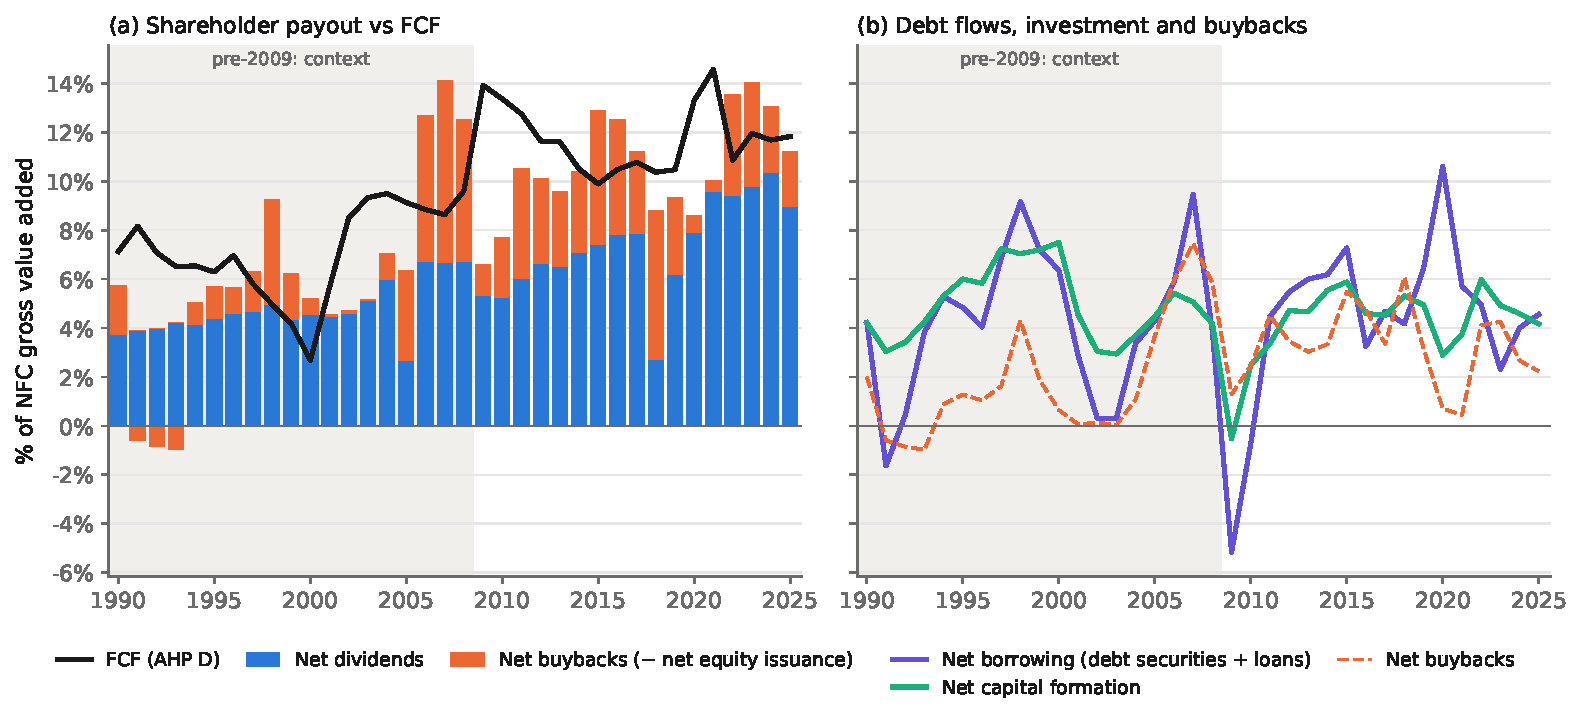
\includegraphics[height=0.47\textheight]{figures/b_f3_nfc_flows.pdf}}
\vspace{-0.15cm}
\begin{columns}[T]
\column{0.5\textwidth}
{\scriptsize\setlength{\tabcolsep}{4pt}
\begin{tabular}{@{}lrrr@{}}\toprule
Mean, \% of GVA & 1990--2007 & 2009--25 & 2011--25\\\midrule
FCF ($D$) & \vb{avg_pre_FCF} & \vb{avg_post_FCF} & \vb{avg_postB_FCF}\\
Net dividends & \vb{avg_pre_DIV} & \vb{avg_post_DIV} & \vb{avg_postB_DIV}\\
Net buybacks & \vb{avg_pre_BUY} & \vb{avg_post_BUY} & \vb{avg_postB_BUY}\\
Net borrowing & \vb{avg_pre_NB} & \vb{avg_post_NB} & \vb{avg_postB_NB}\\
Net capital formation & \vb{avg_pre_NCF} & \vb{avg_post_NCF} & \vb{avg_postB_NCF}\\\bottomrule
\end{tabular}}
\column{0.46\textwidth}
{\scriptsize Cumulated 2009--25 (tn USD): net borrowing \vb{cum_NB}, net capital formation \vb{cum_NCF}, net buybacks \vb{cum_BUY}, net dividends \vb{cum_DIV}. Against this, $Q$ rose by \vb{cum_dQ} tn and equity at market value by \vb{cum_dEQ} tn. Four quarters to \vb{latest_q}: net borrowing \vb{lat_NBY}\%, NCF \vb{lat_NCFY}\%, net buybacks $\vb{lat_BUYY}$\% (net issuance).\par}
\end{columns}
\src{Z.1 F.103 via FRED: BOGZ1FU104104005Q, BOGZ1FU103164103Q (net buybacks $=-$net equity issuance, includes cash-financed M\&A retirements), BOGZ1FU106121075Q, BOGZ1FU105050985Q; four NSA quarters summed. 2018: TCJA repatriation lowers net dividends.}
\end{frame}

\begin{frame}[label=fr-fcf]{II. Where FCF goes: almost all of it to shareholders}{The cash-flow identity of \slref{fr-acct}, NFC sector, Z.1 table S.5.a (closes exactly)}
\centerline{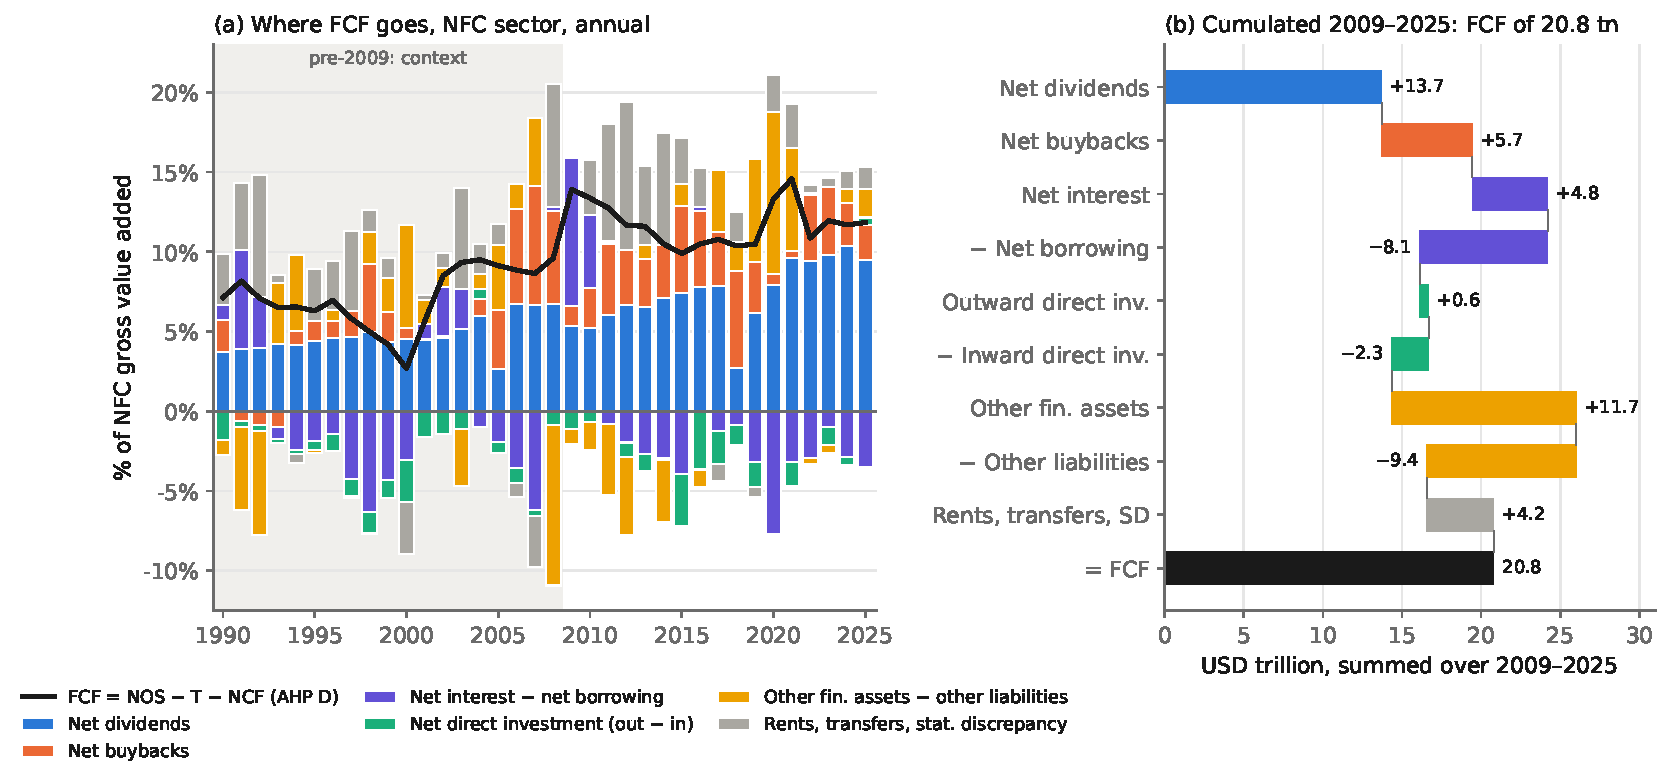
\includegraphics[height=0.46\textheight]{figures/b_f6_fcf_decomposition.pdf}}
\vspace{-0.15cm}
\begin{columns}[T]
\column{0.55\textwidth}
{\scriptsize\setlength{\tabcolsep}{2.2pt}\renewcommand{\arraystretch}{0.9}
\begin{tabular}{@{}lrrr@{}}\toprule
Mean, \% of GVA & 1990--2007 & 2009--25 & 2011--25\\\midrule
FCF $=\mathrm{NOS}-T-\mathrm{NCF}$ & \vb{fd_avg_pre_FCF} & \vb{fd_avg_post_FCF} & \vb{fd_avg_postB_FCF}\\
\quad Div $+$ BB & \vb{fd_avg_pre_DIV} $+$ \vb{fd_avg_pre_BUY} & \vb{fd_avg_post_DIV} $+$ \vb{fd_avg_post_BUY} & \vb{fd_avg_postB_DIV} $+$ \vb{fd_avg_postB_BUY}\\
\quad Int $-\,\Delta$Debt & \vb{fd_avg_pre_INT} $-$ \vb{fd_avg_pre_NB} & \vb{fd_avg_post_INT} $-$ \vb{fd_avg_post_NB} & \vb{fd_avg_postB_INT} $-$ \vb{fd_avg_postB_NB}\\
\quad Net direct investment & $\vb{fd_avg_pre_NDI}$ & $\vb{fd_avg_post_NDI}$ & $\vb{fd_avg_postB_NDI}$\\
\quad Other FA $-$ other liab. & \vb{fd_avg_pre_NOF} & \vb{fd_avg_post_NOF} & \vb{fd_avg_postB_NOF}\\
\quad Rent, Tr, KT, SD & \vb{fd_avg_pre_OTH} & \vb{fd_avg_post_OTH} & \vb{fd_avg_postB_OTH}\\\bottomrule
\end{tabular}}
\column{0.42\textwidth}
{\scriptsize 2009--25 (tn USD): $\mathrm{NOS}-T=\vb{fd_cuma_NOS_T}$ against $\mathrm{NCF}=\vb{fd_cuma_NCF}$, so internal funds alone covered net investment and left FCF $=\vb{fd_cuma_FCF}$. Shareholders received \vb{fd_cuma_DEQ} (\vb{fd_cuma_share_payout}\% of FCF; \vb{fd_cumb_share_payout}\% over 2011--25). Creditors put money in on net: borrowing \vb{fd_cuma_NB} $>$ interest \vb{fd_cuma_INT}. Gross acquisition of financial assets is \vb{fd_cuma_NAFA}, but other liabilities rose \vb{fd_cuma_OL}: net of them, other financial saving is only \vb{fd_cuma_NOF}.\par}
\end{columns}
\src{Z.1 S11.1.i.a (= S.5.a), annual, release of 10 Sep 2026. Div, Int: paid $-$ received. Direct investment: equity flows excluding reinvested earnings (outward $-$ inward). Other liabilities: all except debt securities, loans, corporate equities and FDI equity. Div differs from the FRED net dividends of \slref{fr-flows} by at most \vb{fd_div_diff} tn a year.}
\end{frame}

\begin{frame}[label=fr-bounds]{II. Where firm borrowing went: a range, not a point}{Compustat US nonfinancial firms: positive net borrowing split by use inside each firm-year}
\centerline{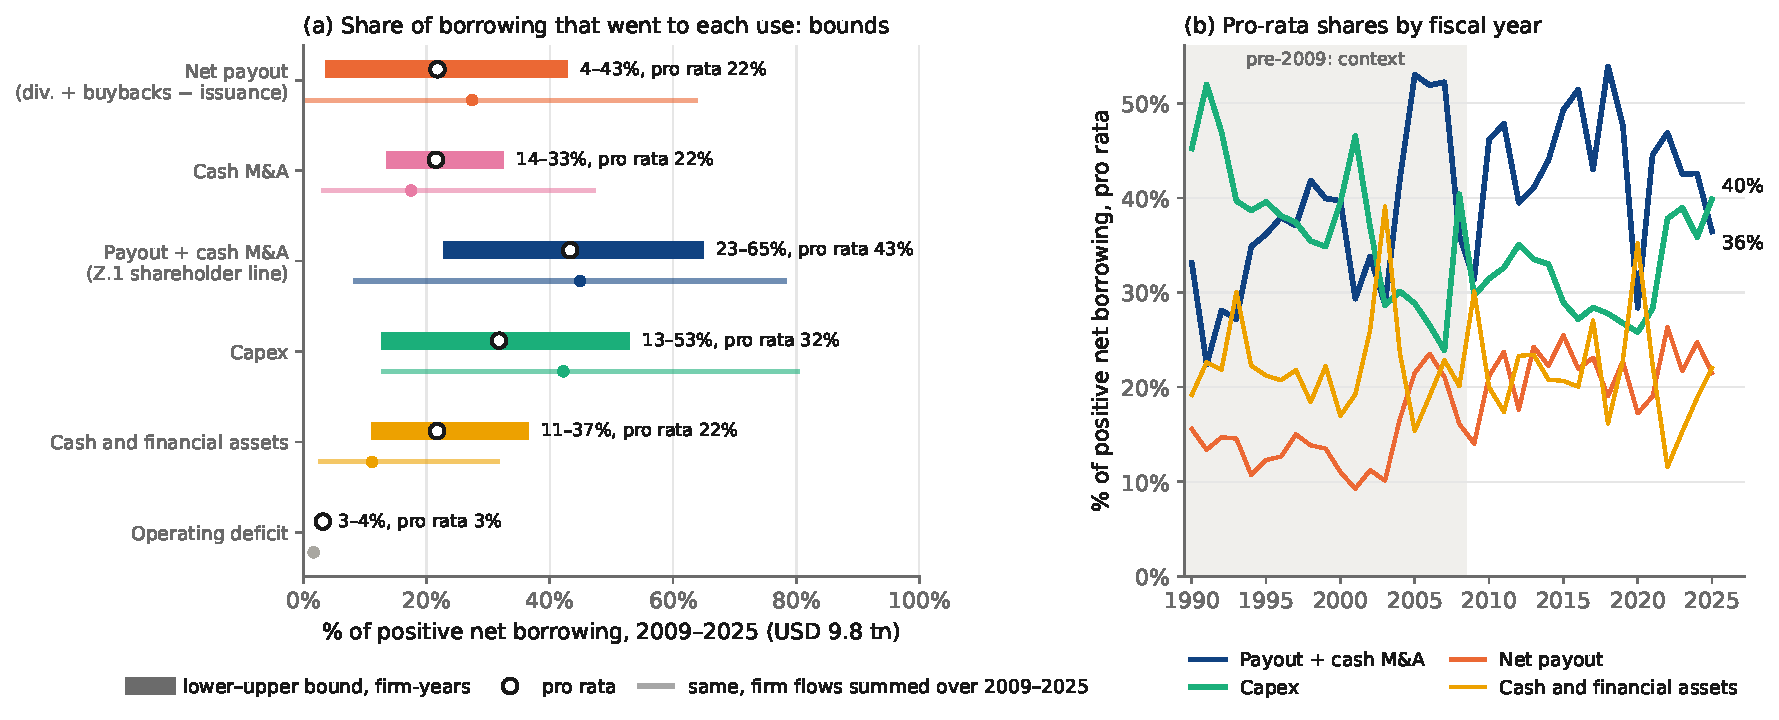
\includegraphics[height=0.46\textheight]{figures/b_f7_debt_use_bounds.pdf}}
\vspace{-0.15cm}
\begin{columns}[T]
\column{0.5\textwidth}
{\scriptsize \textbf{How the bounds work.} Each firm-year: OCF $+$ net borrowing $=$ capex $+$ cash M\&A $+$ net payout $+$ cash and other financial uses. Money is fungible inside a firm, so a use's share of the borrowing is only bounded: \emph{lower} if internal funds pay that use first, \emph{upper} if they pay it last; \emph{pro rata} splits the borrowing in proportion to the uses. Firms with positive net borrowing raised \$\vb{du_ndp} tn in 2009--25; the others repaid \$\vb{du_ndm} tn (net \$\vb{du_nd_net} tn; Z.1 NFC \$\vb{cum_NB} tn).\par}
\column{0.46\textwidth}
{\scriptsize \textbf{What is robust.} Only \vb{du_PAY_lo}\% of the borrowing must have paid shareholders, against \vb{du_INV_lo}\% for capex and \vb{du_MA_lo}\% for cash M\&A. Pro rata, payout + cash M\&A (the Z.1 shareholder line) takes \vb{du_PAYMA_pr}\% and capex \vb{du_INV_pr}\%, but the ranges overlap. Debt paid \vb{du_paydebt_lo}--\vb{du_paydebt_hi}\% of payouts (\vb{du_paydebt_pr}\% pro rata). Capex's pro-rata share: \vb{du_inv_pr_min_pre}--\vb{du_inv_pr_max_pre}\% a year to 2021, \vb{du_inv_pr_min_ai}--\vb{du_inv_pr_max_ai}\% in 2022--25.\par}
\end{columns}
\src{Compustat funda as on \slref{fr-payout}, oancf reported: \vb{du_nfy} firm-years, \vb{du_nfirms} firms. Net borrowing $=$ dltis $-$ dltr $+$ dlcch; net payout $=$ dvt $+$ prstkc $-$ sstk; cash M\&A $=$ aqc; cash and other is the residual. Gross payout: payout \vb{dug_PAY_lo}--\vb{dug_PAY_hi}\%; R\&D as investment: capex $+$ R\&D \vb{dur_INV_lo}--\vb{dur_INV_hi}\%. Global consolidated firms; Z.1 is domestic.}
\end{frame}

\begin{frame}[label=fr-ai]{II. The AI cycle: debt-financed capex since late 2025}{MSFT, GOOGL, AMZN, META, ORCL (and CoreWeave), Compustat quarterly}
\centerline{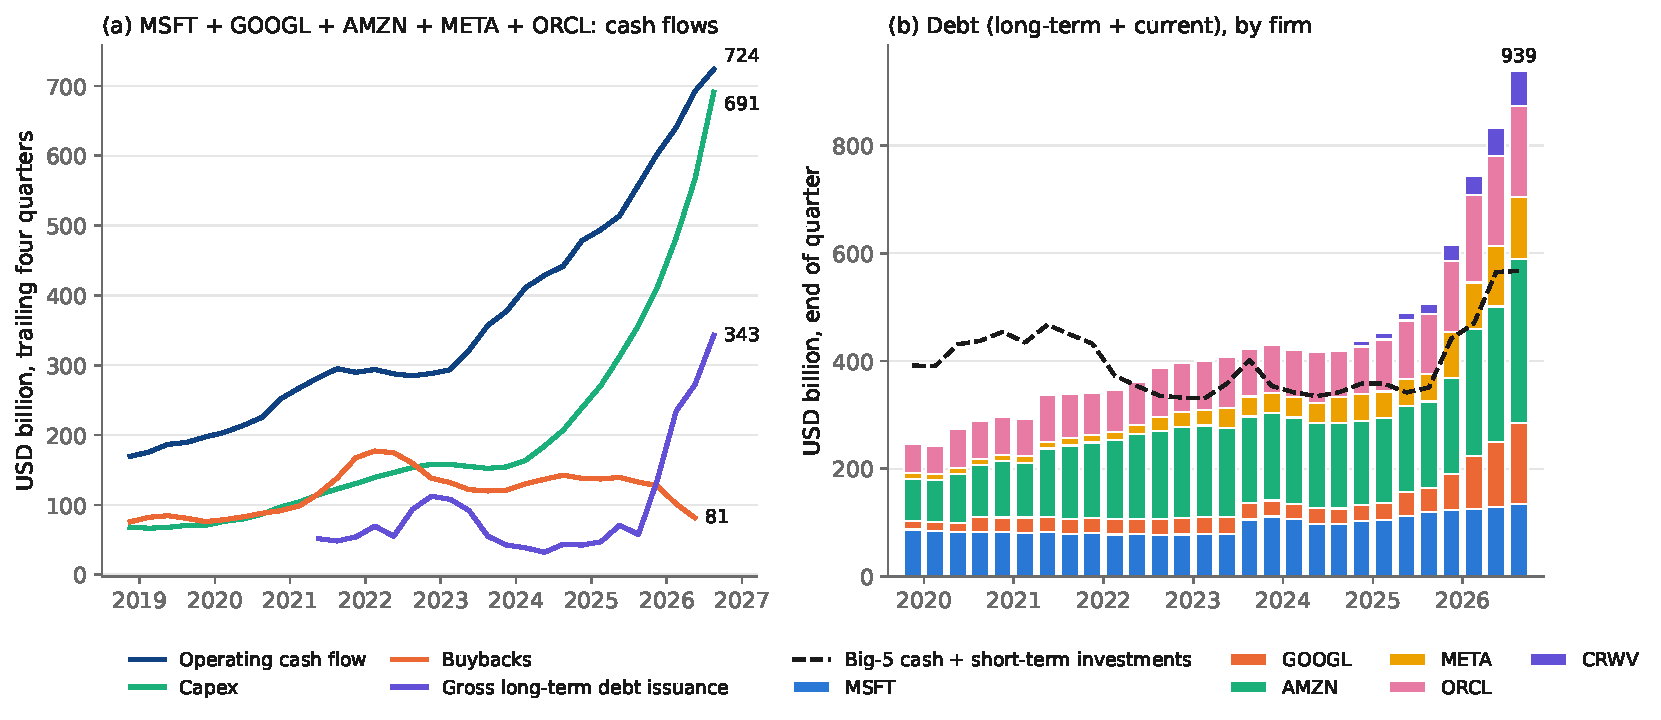
\includegraphics[height=0.47\textheight]{figures/b_f5_ai_hyperscalers.pdf}}
\vspace{-0.1cm}
\begin{columns}[T]
\column{0.5\textwidth}
{\scriptsize\setlength{\tabcolsep}{3pt}
\begin{tabular}{@{}lrrrr@{}}\toprule
Big five, USD bn & 2019Q4 & 2023Q4 & 2025Q4 & \vb{ai_last_q}\\\midrule
Capex, trailing 4Q & \vb{b5_capx_2019q4} & \vb{b5_capx_2023q4} & \vb{b5_capx_2025q4} & \vb{b5_capx_2026q3}\\
Operating cash flow, 4Q & \vb{b5_oancf_2019q4} & \vb{b5_oancf_2023q4} & \vb{b5_oancf_2025q4} & \vb{b5_oancf_2026q3}\\
Capex / OCF & \vb{b5_ratio_2019q4}\% & \vb{b5_ratio_2023q4}\% & \vb{b5_ratio_2025q4}\% & \vb{b5_ratio_2026q3}\%\\
Debt, end of quarter & \vb{b5_debt_2019q4} & \vb{b5_debt_2023q4} & \vb{b5_debt_2025q4} & \vb{b5_debt_2026q3}\\\bottomrule
\end{tabular}}
\column{0.46\textwidth}
{\scriptsize Until 2024 capex was paid out of operating cash flow and buybacks continued. Since 2025Q4: gross long-term debt issuance \$\vb{b5_dltis_2026q3}bn over four quarters (net \$\vb{b5_netiss_2026q3}bn), buybacks down to \$\vb{b5_buy_2026q2}bn (to \vb{ai_last_qbuy}). CoreWeave debt \$\vb{crwv_debt_last}bn. Their debt rise is \vb{b5_ddebt_share_nb}\% of NFC net borrowing in the four quarters to \vb{latest_q}, but their debt is \vb{b5_debt_share_nfc}\% of NFC debt.\par}
\end{columns}
\src{Compustat fundq; flows from fiscal year-to-date items; quarters mapped to calendar quarters by datadate (ORCL ends one month earlier). Debt = dlttq + dlcq; cash = cheq. Global consolidated firms; Z.1 NFC is domestic, so the shares against NFC aggregates are orders of magnitude. Off-balance-sheet data-center financing (joint ventures, leases not yet commenced) is not in these numbers.}
\end{frame}

% ================================================================ PART III
\begin{frame}[label=fr-left]{III. What is left: a rise in $q$, concentrated in a few large firms}{NFC sector (Z.1) and Compustat US nonfinancial firms; candidates are not tested here}
\vspace{0.05cm}
\begin{columns}[T]
\column{0.48\textwidth}
{\small\textbf{What the rise is}}
{\footnotesize
\begin{itemize}\setlength{\itemsep}{0.07cm}
\item \textbf{A price, not a quantity.} Tobin's $q=Q/K$: \vb{q2009} (2009), \vb{q2011} (2011), \vb{q2025} (2025): \vb{dec2009_sh_q}\% of $\Delta\log(Q/Y)$ from 2009, \vb{dec2011_sh_q}\% from 2011 (\slref{fr-capital}).
\item \textbf{Revaluation, not new money.} $Q$ rose \$\vb{sf2009_Q_change} tn from end-2009; net new money from all claim holders was \$\vb{sf2009_Q_flows} tn, so \vb{sf2009_Q_reval_share}\% is revaluation (\vb{sf2011_Q_reval_share}\% from end-2011; \slref{xlink}). Firms retired a net \$\vb{sf2009_E_flows_abs} tn of their own shares.
\item \textbf{Concentrated.} Seven AI-related firms are \vb{ai7_me_share2009}\% of Compustat nonfinancial market equity in 2009, \vb{ai7_me_share2025}\% in 2025, and \vb{ai7_share_dme}\% of its rise.
\item \textbf{Not paid to skilled labor.} $B_H/Y$ rises a little; $B_H/Q$ falls from \va{feBHQ2009} to \va{feBHQ2023} (total corporate, \slref{fr-free}).
\end{itemize}}
\column{0.48\textwidth}
{\small\textbf{Candidates for the rise in $q$}}
{\footnotesize
\begin{enumerate}\setlength{\itemsep}{0.07cm}
\item \textbf{Rents and markups.} Higher rents raise the value of claims without raising $K$. With corporate capital in the accounting, the markup is $\imp{\mu}=1.45$--$1.73$, inside the external range 1.10--1.84 (\slref{fr-corpcap}).
\item \textbf{Unmeasured intangibles.} $K$ at replacement cost excludes organization capital, brands and data; capitalized IPP rises from \vb{IPPY2009}\% to \vb{IPPY2025}\% of NFC GVA. Part of $q$ may be unmeasured capital rather than price.
\item \textbf{A lower required return (funding side).} A stable $\zeta\approx\va{zmean}$ acts as a higher effective $\beta$ (\slref{fr-zeta}); the external position moves through valuation (\slref{fr-ext}).
\end{enumerate}}
\end{columns}
\src{Market equity: Compustat funda, ME = csho$\times$prcc\_f, fiscal year-end; AI-related seven: AAPL, MSFT, GOOGL, AMZN, META, NVDA, ORCL. Revaluation: Z.1 S11.1.i.a levels, transactions and revaluations. Markups: 16 Nov deck, an accounting illustration, not an estimate.}
\end{frame}

\begin{frame}[label=fr-model]{For discussion: what this means for the model}
\vspace{0.1cm}
\begin{columns}[T]
\column{0.48\textwidth}
{\footnotesize
\textbf{What the data support, 2009--2025}
\begin{itemize}\setlength{\itemsep}{0.06cm}
\item No dividend collapse: the rise in $Q/D$ is a rise in $Q/Y$ with $D/Y$ flat (total corporate); including buybacks raises $D/Y$ (NFC).
\item No credit or measured-capital channel: NFC Debt$/Y$ and $K/Y$ are flat, internal funds covered net investment, and \vb{fd_cuma_share_payout}\% of FCF went to shareholders.
\item The funding ratio is stable at $\zeta\approx\va{zmean}$, not converging to 1; RoW net purchases stay near \va{x_purch_post}\% of GVA a year; the quantity of US equity it holds grows no faster than GVA ($\times$\va{x_qtyL} vs $\times$\va{x_gva}); the external position moves through valuation.
\item Skilled labor and investment grow; free entry with constant $a$ and a GVA without capital do not fit.
\end{itemize}}
\column{0.48\textwidth}
{\footnotesize
\textbf{Options, smallest change first}
\begin{enumerate}\setlength{\itemsep}{0.06cm}
\item Reinterpret: $\zeta$ enters only as $\beta\zeta$, so a stable $\zeta\approx1.3$ acts as a higher effective $\beta$. Target the pattern of $Q/Y$, $\zeta$ and the stable quantity share in the external block.
\item Relax the funding cap so the wealth stock can finance $Q$ (bequests, longer lives).
\item Let $a_t$ decline (fishing out) or add convex entry costs, for the free-entry trend.
\item Add corporate capital, so that $D$ maps to FCF and $\mu\approx1.5$.
\end{enumerate}}
\end{columns}
\vfill
{\scriptsize\textcolor{inksec}{The AI cycle (2025--26) is the first episode in the window where capex and debt rise together (\slref{fr-ai}); it can be tracked quarter by quarter in Z.1 and Compustat. Questions: is the 2009+ window, against AHP's 2007 comparison, the right framing for the contribution? Which restriction do we relax first: the funding cap or free entry?}\par}
\vspace{0.3cm}
\end{frame}

% ================================================================ APPENDIX
\begin{frame}[label=fr-topcode]{Appendix: the CPS skill premium in 2023--24, what changed}{Data measurement: the weekly-earnings top code (CPS MORG)}
\centerline{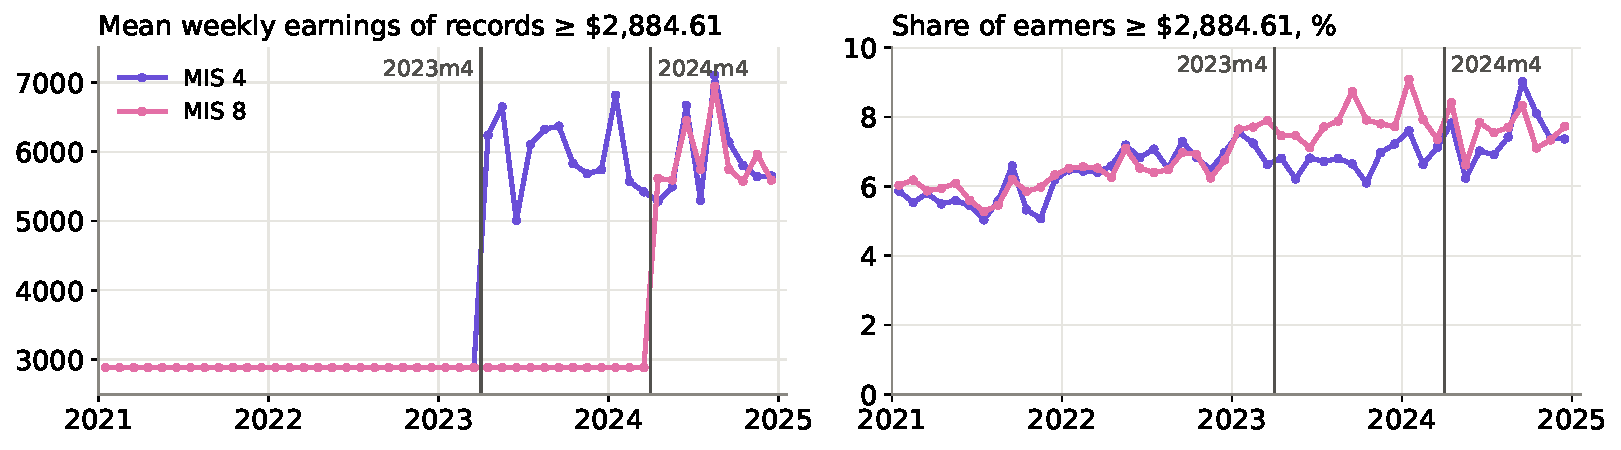
\includegraphics[width=0.78\textwidth]{figures/a_f_topcode_monthly.pdf}}
\vspace{0.05cm}
\begin{columns}[T]
\column{0.49\textwidth}
{\footnotesize
\begin{itemize}\setlength{\itemsep}{0.1cm}
\item \textbf{Before.} CPS outgoing-rotation weekly earnings are top-coded at a fixed \$2,884.61 ($=\$150{,}000/52$): anyone earning more is recorded at exactly that value (flat lines, left).
\item \textbf{The change.} A dynamic rule: the top 3\% of earners get the mean of the top 3\%, about \$9--11k. Rotation group MIS~4 from 2023m4; all records (MIS~8 too) from 2024m4.
\end{itemize}}
\column{0.47\textwidth}
{\footnotesize
\begin{itemize}\setlength{\itemsep}{0.1cm}
\item \textbf{Consequence.} The mean above the old cap jumps to about \$6k, for half the sample in 2023 and all of it in 2024, while the share above the cap moves smoothly (right): a recording change, not an economic one.
\item A mean-wage premium therefore picks up the BA+ upper tail in 2023--24 only.
\end{itemize}}
\end{columns}
\src{NBER CPS MORG 2021--2024, records with positive weekly earnings, earnings weights. Rule change: Census, via IPUMS EARNWEEK2 notes; checked against the MORG files on 2026-10-26.}
\end{frame}

\begin{frame}[label=fr-premium]{Appendix: the skill premium in 2023--24, effect of the top code}{College / non-college mean hourly wage ratio, CPS MORG, fixed 2007 composition}
\centerline{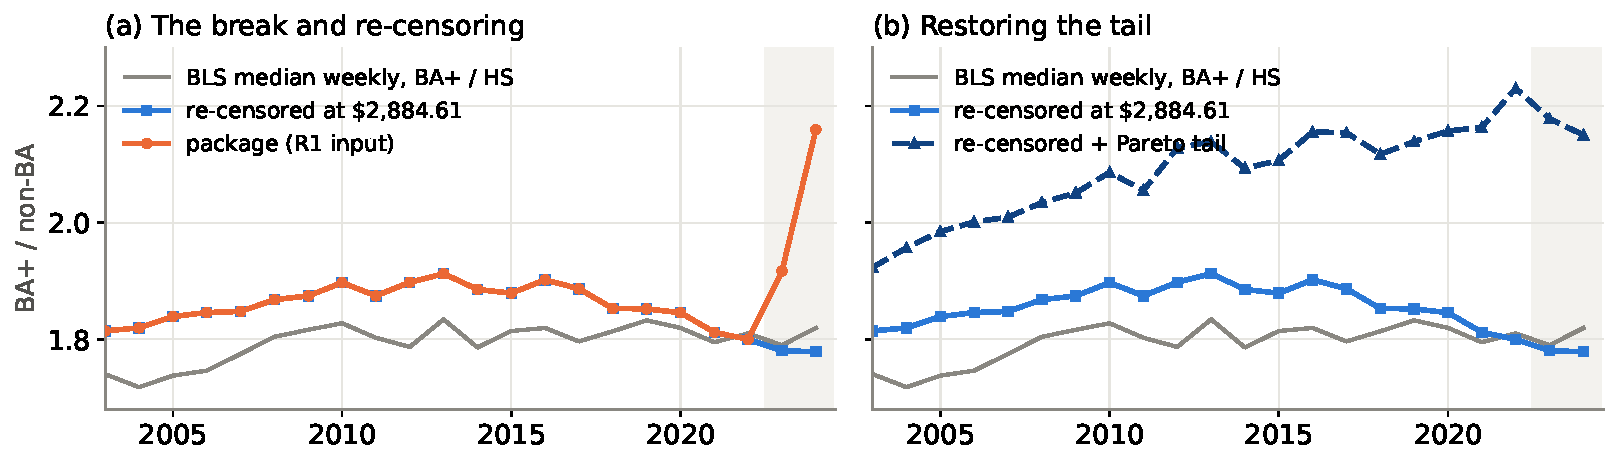
\includegraphics[width=0.66\textwidth]{figures/a_f_premium_treatments.pdf}}
\begin{columns}[T]
\column{0.49\textwidth}
{\scriptsize
\textbf{Re-censoring removes the jump}
\begin{itemize}\setlength{\itemsep}{0.05cm}
\item Package (R1 input): \va{sp_pkg2022}, \va{sp_pkg2023}, \va{sp_pkg2024} (2022--24). Re-censored at \$2,884.61 in every year: \va{sp_rc2022}, \va{sp_rc2023}, \va{sp_rc2024}. In 2023, MIS~4 gives 2.098, and 1.780 re-censored, the same as MIS~8.
\item \textbf{But a fixed nominal cap biases the trend down.} BA+ workers above it rise from 10\% to 24\% (ACS, 2009--24). With the tail restored (Pareto, panel b): \va{sp_par2009} to \va{sp_par2024}; uncapped ACS hourly: 2.086 to 2.173.
\end{itemize}}
\column{0.47\textwidth}
{\scriptsize
\textbf{The BLS median as a check}
\begin{itemize}\setlength{\itemsep}{0.05cm}
\item \textbf{Role.} The BA+ median is far below the cap, so the median ratio is untouched by the top code: \va{sp_bls_min}--\va{sp_bls_max} over 2009--24, no jump in 2023--24. The jump is an artifact.
\item \textbf{Limits.} (i) The model needs a mean, $B_H=w_HH$; the median ignores the upper tail, where much of the BA+ wage bill is, so it understates the premium and its trend (the uncapped mean rises, the median is flat). (ii) BA+ vs high-school graduates only, full-time workers 25+, weekly, no composition adjustment.
\end{itemize}}
\end{columns}
\vspace{0.05cm}
{\scriptsize\textcolor{inksec}{For the premium trend, use the ACS, or KLEMS through 2023 (KLEMS has its own 2024 break, \va{k_prem2023} to \va{k_prem2024}).}}
\src{CPS MORG 2003--2024, private for-profit wage and salary workers 16+. BLS median: FRED LEU0252918500A / LEU0252917300A. ACS 1-year PUMS.}
\end{frame}

\begin{frame}[label=fr-gvatn]{Appendix: GVA by use, trillion USD}{US total corporate GVA (AHP); compensation split with the KLEMS college share}
\centerline{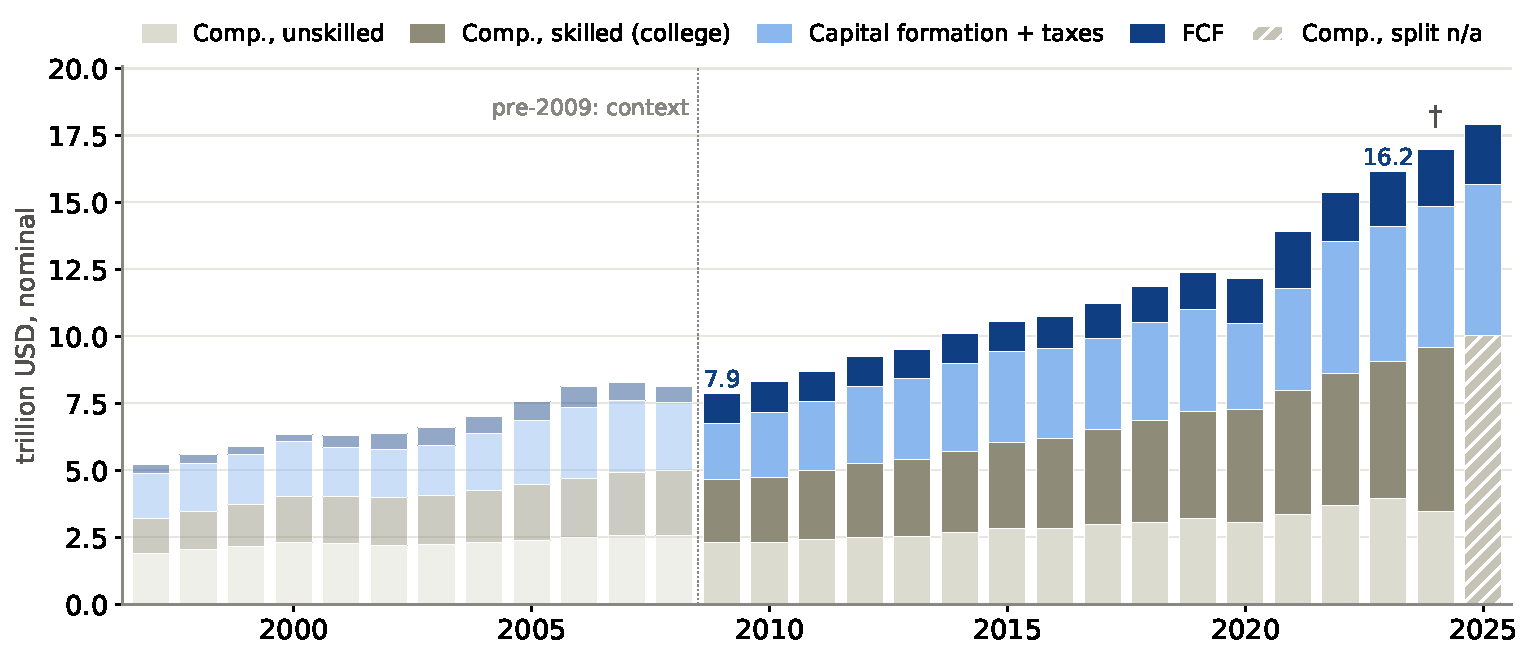
\includegraphics[width=0.82\textwidth]{figures/a_f_gva_values.pdf}}
\vspace{0.05cm}
{\small From 2009 to 2023 nominal GVA rises from \va{Y_tn2009} to \va{Y_tn2023} tn USD (+\va{Y_dtn} tn). Capital formation and taxes add \va{g_kap_dtn} tn, skilled compensation \va{g_skilled_dtn} tn, unskilled compensation \va{g_unskilled_dtn} tn and FCF \va{g_fcf_dtn} tn.}
\src{Capital formation and taxes $=Y-\mathrm{COMP}-\mathrm{FCF}$, i.e.\ CFC $+$ taxes on production and income $+$ net capital formation. \dag\ 2024: likely KLEMS source break. 2025: no KLEMS split yet. Source: figure\_data.csv; BEA--BLS KLEMS, April 2026 release. Total-corporate GVA; the NFC GVA of Part II is smaller.}
\end{frame}

\begin{frame}[label=fr-contrib]{Appendix: contributions to GVA growth, and why the KLEMS split}{US total corporate sector (AHP), 2009 to 2023}
\vspace{0.1cm}
\begin{columns}[T]
\column{0.51\textwidth}
{\scriptsize\setlength{\tabcolsep}{2.4pt}
\begin{tabular}{@{}lrrrrrr@{}}\toprule
 & \multicolumn{3}{c}{tn USD} & of $\Delta Y$ & \multicolumn{2}{c}{of $Y$}\\
 & 2009 & 2023 & $\Delta$ & & 2009 & 2023\\\midrule
Skilled comp. & \va{g_skilled_tn2009} & \va{g_skilled_tn2023} & \va{g_skilled_dtn} & \va{g_skilled_contrib}\% & \va{g_skilled_sh2009}\% & \va{g_skilled_sh2023}\%\\
Unskilled comp. & \va{g_unskilled_tn2009} & \va{g_unskilled_tn2023} & \va{g_unskilled_dtn} & \va{g_unskilled_contrib}\% & \va{g_unskilled_sh2009}\% & \va{g_unskilled_sh2023}\%\\
Capital form.\ + taxes & \va{g_kap_tn2009} & \va{g_kap_tn2023} & \va{g_kap_dtn} & \va{g_kap_contrib}\% & \va{g_kap_sh2009}\% & \va{g_kap_sh2023}\%\\
FCF & \va{g_fcf_tn2009} & \va{g_fcf_tn2023} & \va{g_fcf_dtn} & \va{g_fcf_contrib}\% & \va{g_fcf_sh2009}\% & \va{g_fcf_sh2023}\%\\\midrule
GVA $Y$ & \va{Y_tn2009} & \va{Y_tn2023} & \va{Y_dtn} & 100\% & & \\\bottomrule
\end{tabular}}\\[0.25cm]
{\small Capital formation and taxes and skilled compensation each account for about a third of the rise in GVA. Inside the capital bucket, net capital formation goes from \va{ncf2009}\% to \va{g_ncf_sh2023}\% of GVA and taxes on income from \va{inctax2009}\% to \va{inctax2023}\%; CFC cannot be separated from production taxes in the current data.}
\column{0.46\textwidth}
{\small\textbf{Why KLEMS rather than CPS or ACS}}\\[0.1cm]
{\scriptsize\setlength{\tabcolsep}{4pt}
\begin{tabular}{@{}lrr@{}}\toprule
Skilled share of compensation & 2009 & 2023\\\midrule
KLEMS (published by education) & \va{ss_klems2009}\% & \va{ss_klems2023}\%\\
ACS bridge (annual earnings) & \va{ss_acs2009}\% & \va{ss_acs2023}\%\\
CPS bridge (hourly premium) & \va{ss_cps2009}\% & \va{ss_cps2023}\%\\
STEM occupations & \va{ss_stem2011}\%$^{*}$ & \va{ss_stem2023}\%\\\bottomrule
\end{tabular}}\\[0.15cm]
{\scriptsize
\begin{itemize}\setlength{\itemsep}{0.04cm}
\item \textbf{KLEMS} publishes college and non-college compensation by industry, with totals controlled to NIPA; no premium-times-headcount bridge. The split still uses survey earnings (Census PUMS, CPS March), so it is less exposed to top codes, not immune.
\item \textbf{CPS}: hourly premium times headcounts misses BA+ hours, and the top code compresses high earners (break in 2023--24, \slref{fr-topcode}); 7--10\,pp below KLEMS.
\item \textbf{ACS}: annual earnings, close to KLEMS after 2009; a cross-check.
\end{itemize}}
\end{columns}
\src{KLEMS: private industries incl.\ noncorporate; share applied to corporate compensation. $^{*}$STEM: occupation-based $H$, from 2011. Ends 2023 (2024 break).}
\end{frame}

\begin{frame}[label=fr-corpcap]{Appendix: corporate capital}{US total corporate sector (AHP); the model has no place for depreciation, taxes and investment}
\vspace{0.1cm}
\begin{columns}[T]
\column{0.5\textwidth}
{\small Non-labor income, data vs model:
\[
\underbrace{\mathrm{CFC}+\mathrm{Taxes}+\mathrm{NCF}+\mathrm{FCF}}_{\text{data: }Y-\mathrm{COMP}}
\;=\;\underbrace{\D-\I\;=\;Y-e}_{\text{model}}
\]
\begin{tabular}{@{}lr@{}}\toprule
Share of corporate GVA, mean 2009--25 & \\\midrule
Compensation & \va{avg_comp}\%\\
CFC + taxes & \va{avg_cfctax}\%\\
Net capital formation (NCF) & \va{avg_ncf}\%\\
FCF ($=$ AHP $D$) & \va{avg_fcf}\%\\\midrule
Non-labor income $Y-\mathrm{COMP}$ & \va{avg_nonlab}\%\\\bottomrule
\end{tabular}}
\column{0.46\textwidth}
{\small
\begin{itemize}\setlength{\itemsep}{0.2cm}
\item The model must route all \va{avg_nonlab}\% into net payout $\D-\I$; in the data only FCF, about \va{avg_fcf}\%, is payable to owners. CFC is replacement investment: gross investment $=$ CFC $+$ NCF.
\item \textbf{Markup.} P1 then implies $\imp{\mu}=\bigl(1+(Y-\mathrm{COMP})/B_H\bigr)/\varphi=2.34$--$3.02$. If capital absorbs CFC, taxes and NCF, $\imp{\mu}=(1+\mathrm{FCF}/B_H)/\varphi=1.45$--$1.73$, inside the external range 1.10--1.84 (DLEU: 1.61).
\item \textbf{Valuation.} $Q$ is enterprise value and includes installed capital, so $B_H/Q$ on \slref{fr-free} also mixes in capital.
\end{itemize}}
\end{columns}
\src{Shares from figure\_data.csv; CFC and taxes are the GVA residual. Markups: 2009--24, NSCG $\varphi$, three premium series (2\_Check/On\_Model\_vs\_Data\_Failed\_Dimensions.md, Section 2.2); an accounting illustration, not an estimate.}
\end{frame}

\begin{frame}[label=xvalue]{Appendix: the value side of \slref{fr-acct}, explained}{What $Q$ measures, and why it is split by type of claim; NFC sector (Z.1)}
\vspace{-0.15cm}
\begin{columns}[T]
\column{0.47\textwidth}
{\scriptsize\textbf{Market-value balance sheet, NFC, end-2025 (USD tn)}\\[0.08cm]
\setlength{\tabcolsep}{2pt}
\begin{tabular}{@{}lr|lr@{}}\toprule
\multicolumn{2}{@{}l|}{\textbf{What firms own}} & \multicolumn{2}{l@{}}{\textbf{Claims on firms}}\\\midrule
\textcolor{dataD}{\textbf{Nonfinancial assets $Q$}} & \textcolor{dataD}{\textbf{\vb{bs2025_Q}}} & Equity $E$ & \vb{bs2025_E}\\
\quad\textcolor{inksec}{(backed out)} & & Foreign parents, FDI$^{mv}$ & \vb{bs2025_FDI}\\
Financial assets FA & \vb{bs2025_FA} & Debt & \vb{bs2025_DEBT}\\
 & & Other liabilities OL & \vb{bs2025_OL}\\\midrule
Total & \vb{bs2025_TOT} & Total & \vb{bs2025_TOT}\\\bottomrule
\end{tabular}\\[0.12cm]
Market prices exist for the claims on the right, not for the factories, software and brands on the left. Z.1 therefore backs $Q$ out of the two totals:
\[Q=E+\mathrm{FDI}^{mv}+\mathrm{Debt}+\mathrm{OL}-\mathrm{FA}.\]
\textcolor{inksec}{FDI$^{mv}$: equity of foreign parents in their US affiliates. FA: cash and deposits, receivables, securities, US firms' equity in their foreign affiliates. OL: trade and tax payables, pension liabilities, intercompany debt owed to foreign parents.}\par}
\column{0.49\textwidth}
{\scriptsize
\begin{itemize}\setlength{\itemsep}{0.03cm}
\item \textbf{What $Q$ is.} The price of the whole business: buy every share, take over every debt and payable, keep the cash and other financial assets.
\item \textbf{Why it is the model's $Q$.} In the model the firm has one claim, worth the present value of future $D$. In the data the cash flows are shared by shareholders, creditors and others; the sum of all claims does not depend on how the firm is financed.
\item \textbf{Why FA is netted out.} Cash and securities are not productive capital; foreign affiliates are not US capital. A firm that borrows to hold cash raises Debt and FA together, and $Q$ does not move.
\item \textbf{Why split by claim.} Divided by $Y$, the terms add up to $Q/Y$, so a change in $Q/Y$ splits exactly by claim: credit shows up in Debt$/Y$, equity (issued or revalued) in $E/Y$. 2009$\to$2025, pp of GVA (\slref{fr-credit}): $Q/Y$ $+\vb{dec2009_dQY_pp}$ $=$ $E$ $+\vb{dec2009_dEY_pp}$, FDI$^{mv}$ $+\vb{dec2009_dFDIY_pp}$, Debt $+\vb{dec2009_dDEBTY_pp}$, OL$-$FA $\vb{dec2009_dOTHERY_pp}$.
\item \textbf{What it cannot say.} A debt-financed buyback swaps $E$ for Debt one for one, so the split shows which claims grew, not why. Telling new money from price changes needs the flows (\slref{xlink}).
\end{itemize}}
\end{columns}
\src{Z.1 B.103/L.103 via FRED, as on slides \ref{fr-acct}--\ref{fr-credit}; the identity is the Fed's definition of FL102010405 (market value estimate of nonfinancial assets). Unlisted firms' equity is not traded; its market value is a Fed estimate.}
\end{frame}

\begin{frame}[label=xcash]{Appendix: the cash-flow side of \slref{fr-acct}, explained}{What FCF measures, and why it is split by who receives it}
\vspace{-0.15cm}
\begin{columns}[T]
\column{0.41\textwidth}
{\scriptsize\textbf{Worked example: one firm, one year}\\[0.05cm]
Operating surplus after wages, production taxes and depreciation (NOS) 100; income tax 20; net investment 30; interest 5. So $\mathrm{FCF}=100-20-30=50$, whatever the firm does next:\\[0.03cm]
\setlength{\tabcolsep}{4pt}
\begin{tabular}{@{}lrrrr@{}}\toprule
 & (a) & (b) & (c) & (d)\\\midrule
Dividends & 45 & 0 & 45 & 25\\
Buybacks & 0 & 45 & 20 & 0\\
Interest & 5 & 5 & 5 & 5\\
$-$ New borrowing & 0 & 0 & $-20$ & 0\\
Kept as cash & 0 & 0 & 0 & 20\\\midrule
$=$ FCF & 50 & 50 & 50 & 50\\\midrule
To shareholders & 45 & 45 & 65 & 25\\
To creditors & 5 & 5 & $-15$ & 5\\\bottomrule
\end{tabular}\\[0.03cm]
(a) pays dividends; (b) buys back shares instead; (c) also borrows 20 to buy back more; (d) keeps 20 as cash. Dividends alone would fall to 0 in (b), with nothing changed.\par}
\column{0.55\textwidth}
{\scriptsize
\begin{itemize}\setlength{\itemsep}{0.04cm}
\item \textbf{What FCF is.} Cash left after wages, taxes, depreciation and net investment (NCF), before any payment to shareholders or creditors.
\item \textbf{Why it is the model's $D$.} $D$ must be the cash flow of the claims that $Q$ values: all claims, net of financial assets. So $D$ is all payments to them, net of new borrowing and of cash kept: FCF.
\item \textbf{Why not dividends.} US payout has shifted from dividends to buybacks since the 1980s. Dividends alone would show a fall that is only a change of form (column b).
\item \textbf{Why split by recipient.} Does payout form matter (shareholder line)? Did borrowing pay for payouts (sign of the creditor line)? Do firms hoard cash (net financial saving)? 2009--25: \vb{fd_cuma_share_payout}\% of FCF went to shareholders (\slref{fr-fcf}).
\item \textbf{Why it closes exactly.} Income not taxed or invested is paid out or changes financial assets or liabilities. Income data are from BEA, financial data from the Fed; SD is the gap. The identity always holds; the content is in the size of each term.
\item \textbf{What it cannot say.} Money is fungible: the split says how much went to each group, not which source paid for which use. A cash takeover of one US firm by another is a buyback for the sector.
\end{itemize}}
\end{columns}
\src{In the data, ``kept as cash'' is net financial saving, NAFA $-\,\Delta$OL $-$ RE (\slref{fr-acct}): purchases of financial assets, net of other new liabilities and of foreign affiliates' reinvested earnings (earned abroad, so not in NOS). Rent, Tr, KT and SD are the remaining small items (glossary, \slref{fr-gloss1}). Which firm's borrowing paid for which use: \slref{fr-bounds}.}
\end{frame}

\begin{frame}[label=xlink]{Appendix: how the two sides connect}{Change in a stock $=$ net transactions (the cash-flow side) $+$ revaluation; NFC sector (Z.1), USD tn}
\vspace{-0.15cm}
\begin{columns}[T]
\column{0.52\textwidth}
{\scriptsize\setlength{\tabcolsep}{2.5pt}\textbf{End-2009 to end-2025}\\[0.05cm]
\begin{tabular}{@{}lrrrr@{}}\toprule
 & Change & $=$ Net & $+$ Reval- & $+$ Other\\
 & in stock & transactions & uation & changes\\\midrule
Equity, $E$ & $\vb{sf2009_E_change}$ & $\vb{sf2009_E_flows}$ & $\vb{sf2009_E_reval}$ & $\vb{sf2009_E_other}$\\
FDI$^{mv}$ & $\vb{sf2009_FDI_change}$ & $\vb{sf2009_FDI_flows}$ & $\vb{sf2009_FDI_reval}$ & $\vb{sf2009_FDI_other}$\\
Debt & $\vb{sf2009_DEBT_change}$ & $\vb{sf2009_DEBT_flows}$ & -- & $\vb{sf2009_DEBT_other}$\\
Other liabilities, OL & $\vb{sf2009_OL_change}$ & $\vb{sf2009_OL_flows}$ & $\vb{sf2009_OL_reval}$ & $\vb{sf2009_OL_other}$\\
$-$ Financial assets, FA & $\vb{sf2009_MFA_change}$ & $\vb{sf2009_MFA_flows}$ & $\vb{sf2009_MFA_reval}$ & $\vb{sf2009_MFA_other}$\\\midrule
$=Q$ & $\mathbf{\vb{sf2009_Q_change}}$ & $\mathbf{\vb{sf2009_Q_flows}}$ & $\mathbf{\vb{sf2009_Q_reval}}$ & $\vb{sf2009_Q_other}$\\\bottomrule
\end{tabular}\\[0.1cm]
\textcolor{inksec}{Net transactions are the flows of the cash-flow side: new shares minus shares retired ($-$BB), net borrowing, purchases of financial assets (NAFA). Revaluation is the change in the value of a stock that is not a transaction: holding gains and losses (Fed revaluation account). Debt is at book value, so it has none. Other changes: reclassifications, write-offs and breaks in the source data.}\par}
\column{0.44\textwidth}
{\scriptsize
\begin{itemize}\setlength{\itemsep}{0.1cm}
\item \textbf{Equity.} Firms retired a net \$\vb{sf2009_E_flows_abs} tn of their own shares, yet the market value of their equity rose \$\vb{sf2009_E_change} tn. None of the rise came from new shares.
\item \textbf{All claims.} $Q$ rose \$\vb{sf2009_Q_change} tn. Net new money from all claim holders, net of financial assets bought, was \$\vb{sf2009_Q_flows} tn: \vb{sf2009_Q_reval_share}\% of the rise is revaluation (\vb{sf2011_Q_reval_share}\% from end-2011).
\item \textbf{What revaluation contains.} The value of investment paid for out of retained earnings (no new claims are issued for it) and price changes. The capital side separates the two: $K$ at replacement cost rose \$\vb{sf2009_dK} tn, so most of the rise in $Q$ is a rise in $q=Q/K$ (\slref{fr-capital}).
\item \textbf{Why both sides.} The value side alone cannot tell new claims from higher prices; the cash-flow side alone says nothing about prices.
\end{itemize}}
\end{columns}
\src{Z.1 S11.1.i.a (= S.5.a): levels, transactions (FU) and revaluations (FR) from one table; other changes $=$ change $-$ transactions $-$ revaluation. Stocks at end-2009 and end-2025, so flows are summed over 2010--25 (\slref{fr-fcf} sums 2009--25). Rounded to 0.1. From end-2011: $Q$ $+$\vb{sf2011_Q_change}, transactions $+$\vb{sf2011_Q_flows}, revaluation $+$\vb{sf2011_Q_reval}.}
\end{frame}

\begin{frame}[label=fr-sources]{Appendix: sources and rebuild}
\vspace{0.05cm}
{\tiny
\textbf{This deck} merges the 16 Nov deck (Logistics/Discussion\_note/29\_11\_16/slides; \texttt{\textbackslash va} values, figures \texttt{a\_*}) and the 18 Nov deck (Codes/Calibration\_R1/2\_Check/2026\_11\_18\_Credit\_Buybacks; \texttt{\textbackslash vb} values, figures \texttt{b\_*}). New here: the scorecard (\slref{fr-summary}), the sector table (\slref{fr-fact}) and the synthesis figure (\slref{fr-synth}), \texttt{\textbackslash vc} values and \texttt{s\_*} figure. No data were re-fetched.\\[0.1cm]
\textbf{Total corporate sector (AHP).} Codes/Calibration\_R1/2\_Check/figures/figure\_data.csv: AHP total-corporate $Y$, COMP, FCF, EV (Fed Z.1, BEA IMA Tables S.5--S.6), with CPS, ACS, STEM and KLEMS skill splits; labor\_block\_klems.csv; zeta\_funding\_ratio\_1990\_2025.csv.\\[0.1cm]
\textbf{External accounts.} Empirical\_Data/AHP\_NFA (June 2026 release) for purchases, valuation and the quantity of US equity held by RoW. $\zeta$ uses the September 2026 release, with the June-consistent line for comparison; $Q$ and NFA always come from one release.\\[0.1cm]
\textbf{Labor.} BEA--BLS Integrated Industry-Level Production Account, April 2026 release (Empirical\_Data/BEA\_BLS\_KLEMS\_2026-04-27); NBER CPS MORG; ACS 1-year PUMS (Empirical\_Data/Skill\_Premium\_and\_RD\_Share\_2026-10-26).\\[0.1cm]
\textbf{NFC sector.} Z.1 / NIPA via FRED (retrieved 2026-11-18, data through \vb{latest_q}), 30 series; Z.1 table S11.1.i.a (= S.5.a), Fed CSV release of 10 Sep 2026. Annual flows are sums of four NSA quarters; stocks are end of Q4.\\[0.1cm]
\textbf{Compustat} (WRDS, retrieved 2026-11-18): comp.funda for US-incorporated USD filers, fiscal 1989--2026 (2026 not used); comp.fundq for AAPL, MSFT, ORCL, CRWV, AMZN, NVDA, GOOGL, META from 2014. Licensed data: not for redistribution.\\[0.1cm]
\textbf{Model.} AI\_drafting/V6\_production.tex; Two\_country\_proudction\_zero\_nu\_b/outputs\_zero\_nu\_b, notebooks 05--06; model decompositions in 2\_Check/slides/data/decomp\_model.csv.\\[0.1cm]
\textbf{Literature.} Atkeson, Heathcote and Perri, The End of Privilege (AHP); Hirano, Kishi and Toda (2025), arXiv:2501.08215; Bloom, Jones, Van Reenen and Webb (2020), AER; De Loecker, Eeckhout and Unger (2020), QJE.\\[0.1cm]
\textbf{Rebuild} (in this folder; build.py fails if any value key used in the deck is undefined; the two source decks are rebuilt in their own folders, see their READMEs):\\
\texttt{uv run -{}-no-project -{}-python 3.12 -{}-with numpy==2.3.5 -{}-with pandas==2.2.3 -{}-with matplotlib==3.10.0 python -I scripts/build.py}\newline
\texttt{latexmk -pdf qy\_mechanisms\_data\_2026\_11\_19.tex}; \texttt{latexmk -c}\par}
\end{frame}

% ---------------------------------------------------------------- glossary
\newcommand{\gl}[2]{\textbf{#1} & #2\\}
\newcommand{\glbegin}{\tiny\setlength{\tabcolsep}{3pt}\renewcommand{\arraystretch}{1.12}\begin{tabular}{@{}>{\raggedright}p{0.17\linewidth}p{0.79\linewidth}@{}}\toprule}
\newcommand{\glend}{\bottomrule\end{tabular}}
\begin{frame}[label=fr-gloss1]{Appendix: abbreviations and symbols (1/3)}{Accounting terms; flows are annual transactions, stocks end of year}
\vspace{-0.05cm}
\begin{columns}[T]
\column{0.49\textwidth}
{\glbegin
\gl{Total corp.}{US corporate sector, financial and nonfinancial, in the AHP mapping of Z.1 and BEA IMA (Part I)}
\gl{NFC}{Nonfinancial corporate business, the Z.1 sector of Part II}
\gl{$Y$, GVA}{Gross value added of the sector named on the slide}
\gl{$Q$, EV}{Enterprise value: market value of nonfinancial assets $=E+\mathrm{FDI}^{mv}+\mathrm{TL}-\mathrm{FA}$ (NFC: Z.1 FL102010405); the AHP $Q$}
\gl{$E$}{Corporate equities issued by NFCs, market value}
\gl{FDI$^{mv}$}{Foreign direct investment in the US (equity in US affiliates of foreign parents), market value}
\gl{TL, FA}{Total liabilities (excluding equity); total financial assets}
\gl{Debt}{Debt securities (corporate bonds, commercial paper, municipal) $+$ loans (bank, private credit, mortgages, other)}
\gl{OL}{Other liabilities $=\mathrm{TL}-\mathrm{Debt}$: trade payables, taxes payable, pension entitlements, FDI intercompany debt, miscellaneous}
\gl{$K$}{Nonfinancial assets at replacement cost: real estate at market value; equipment, IPP and inventories at current cost}
\gl{$q$}{Tobin's $q=Q/K$ (Part II). With a time subscript in the model, $q_t$ is the price of one variety (\slref{fr-hkt})}
\gl{IPP}{Intellectual property products: R\&D, software, entertainment and artistic originals}
\gl{$D$, FCF}{Free cash flow $=\mathrm{NOS}-T-\mathrm{NCF}$, the AHP dividend measure}
\gl{Payout}{Net dividends $+$ net buybacks (shareholder payout)}
\gl{NOS}{Net operating surplus: GVA $-$ compensation of employees $-$ taxes on production and imports (less subsidies) $-$ consumption of fixed capital}
\glend}
\column{0.49\textwidth}
{\glbegin
\gl{COMP}{Compensation of employees}
\gl{CFC}{Consumption of fixed capital (depreciation at replacement cost)}
\gl{$T$, Taxes}{Current taxes on corporate income, wealth, etc.; ``CFC + taxes'' also includes taxes on production}
\gl{NCF}{Net capital formation: gross fixed investment $+$ inventory change $+$ net purchases of nonproduced assets $-$ CFC}
\gl{Div}{Net dividends: dividends paid $-$ dividends received}
\gl{BB}{Net buybacks $=-$ net issuance of corporate equities (net of IPOs and new issues; includes shares retired in cash M\&A)}
\gl{Int}{Net interest: interest paid $-$ interest received}
\gl{$\Delta$Debt, NB}{Net borrowing: net incurrence of debt securities and loans}
\gl{NAFA}{Net acquisition of financial assets}
\gl{$\Delta$OL}{Net incurrence of OL, plus inward FDI equity flows}
\gl{RE}{Reinvested earnings on direct investment, net: earned by US firms' foreign affiliates $-$ earned by foreign parents on US affiliates. Recorded as income and as a direct-investment flow, but not in NOS}
\gl{Net direct inv.}{Outward direct-investment equity flow $-$ inward FDI equity flow, both excluding reinvested earnings}
\gl{Rent, Tr, KT}{Rents paid on land and natural resources; other current transfers paid; net capital transfers paid}
\gl{SD}{Statistical discrepancy of the NFC accounts (capital-account minus financial-account net lending)}
\glend}
\end{columns}
\end{frame}

\begin{frame}[label=fr-gloss2]{Appendix: abbreviations and symbols (2/3)}{Model symbols (Part I) and external accounts}
\vspace{-0.05cm}
\begin{columns}[T]
\column{0.49\textwidth}
{\glbegin
\gl{HKT}{Hirano, Kishi and Toda, \emph{Technological innovation and bursting bubbles}; the project's model}
\gl{$e$}{Labor compensation $=w_HH+w_LL$ (model income of the young)}
\gl{$H$, $L$}{Skilled (college) and unskilled labor; in the data KLEMS college and non-college labor input}
\gl{$w_H$, $w_L$}{Skilled and unskilled wage; premium $=w_H/w_L$}
\gl{$B_H$, $B_L$}{Skilled and unskilled wage bills, $w_HH$ and $w_LL$}
\gl{$\varphi$, $X$}{Share of skilled labor used in production; $X_t=\varphi_tH$. $1-\varphi$: R\&D share}
\gl{$d_t$, $q_t$}{Dividend and price of one variety}
\gl{$N_t$, $G_t$}{Number of varieties; its gross growth $G_t=N_{t+1}/N_t=1+a(1-\varphi_t)H$}
\gl{$a$}{Research productivity in the knowledge law (free entry: $q_t=w_{H,t}/(aN_t)$)}
\gl{$\vartheta$}{CES parameter of the variety aggregator, $\vartheta\in(0,1)$: price $=w_H/\vartheta$, dividend $=(1-\vartheta)/\vartheta$ times the variety wage bill}
\gl{$\rho$, $\xi_u$, $\nu_u$}{$\rho>1$: inverse elasticity of substitution between $X$ and $L$ in final output; $\xi_u$, $\nu_u$: exponents of the variety spillover on $X$- and $L$-productivity. $u$ regime: $\xi_u>\nu_u$}
\gl{$\beta$, OLG}{Saving rate of the young in the two-period overlapping-generations (OLG) model; funding cap $Q+\mathrm{NFA}=\beta e$}
\gl{$\D$, $\I$, $\Qc$}{Model aggregate dividends, investment (entry cost), and value of firms}
\gl{$\mu$}{Markup implied by the model's first-order condition (P1)}
\gl{$u$ regime}{Unbalanced-growth regime; in the data the 2009--2025 window}
\glend}
\column{0.49\textwidth}
{\glbegin
\gl{NFA}{US net foreign assets}
\gl{$A_t$}{Wealth of the young $=\beta e_t=Q_t+\mathrm{NFA}_t$ with zero-net-supply bonds}
\gl{$\zeta$}{Funding ratio $Q/(Q+\mathrm{NFA})=1-\mathrm{NFA}/A$; HKT tail limit 1}
\gl{RoW}{Rest of the world}
\gl{EL, EA}{US equity liabilities (foreign-held US equity, portfolio $+$ FDI at market value); US equity assets abroad}
\gl{RoW equity quantity}{Quantity of US equity held by RoW: EL over its price index; divided by nominal GVA on \slref{fr-synth}}
\gl{P1}{The model's production first-order condition used to back out $\mu$}
\gl{$\Delta\log$}{Change in natural log between two years; shares of $\Delta\log(Q/D)$ add to 100\%}
\gl{AHP}{Atkeson, Heathcote and Perri, \emph{The End of Privilege}; source of the $Q$ (enterprise value) and $D$ (FCF) mappings}
\gl{BJVW}{Bloom, Jones, Van Reenen and Webb (2020), research productivity, $-5.1$\%/yr}
\gl{DLEU}{De Loecker, Eeckhout and Unger (2020), markups}
\gl{MM}{Modigliani--Miller: financing and payout form do not change firm value or FCF}
\gl{pp}{Percentage points}
\gl{tn, bn}{Trillion, billion (USD, nominal)}
\glend}
\end{columns}
\end{frame}

\begin{frame}[label=fr-gloss3]{Appendix: abbreviations and symbols (3/3)}{Data sources, survey and firm-level terms}
\vspace{-0.05cm}
\begin{columns}[T]
\column{0.49\textwidth}
{\glbegin
\gl{Z.1}{Financial Accounts of the United States (Federal Reserve)}
\gl{B.103, L.103, F.103}{Z.1 tables for the NFC sector: balance sheet, liabilities and assets (levels), flows}
\gl{S.5.a (S11.1.i.a)}{Z.1 integrated macroeconomic accounts for the NFC sector, annual (new table name in brackets)}
\gl{IMA}{Integrated macroeconomic accounts (Fed--BEA)}
\gl{NIPA, BEA}{National Income and Product Accounts; Bureau of Economic Analysis}
\gl{FRED}{Federal Reserve Economic Data (St.\ Louis Fed), used to download Z.1 series}
\gl{FL, FU, LM, FR}{Z.1 series prefixes: level, unadjusted flow (transactions), market-value level, revaluation}
\gl{NSA, SAAR}{Not seasonally adjusted; seasonally adjusted annual rate}
\gl{TTM, 4Q}{Trailing twelve months: sum of the last four quarters}
\gl{KLEMS}{BEA--BLS Integrated Industry-Level Production Account (capital, labor, energy, materials, services), with compensation by education}
\gl{CPS, MORG}{Current Population Survey; its Merged Outgoing Rotation Groups (NBER files)}
\gl{MIS}{Month in sample: CPS rotation group (MIS 4 and MIS 8 carry earnings)}
\gl{ACS, PUMS, IPUMS}{American Community Survey; Public Use Microdata Sample; Integrated Public Use Microdata Series}
\gl{BLS, NSCG}{Bureau of Labor Statistics; National Survey of College Graduates (source of $\varphi$)}
\gl{BA+, HS, STEM}{Bachelor's degree or more; high-school graduates; science, technology, engineering and mathematics occupations}
\glend}
\column{0.49\textwidth}
{\glbegin
\gl{WRDS}{Wharton Research Data Services}
\gl{Compustat}{S\&P firm accounts: funda (annual), fundq (quarterly); global consolidated, whereas Z.1 is domestic}
\gl{prstkc}{Purchase of common and preferred stock (gross buybacks)}
\gl{sstk, dvt}{Sale of common and preferred stock (issuance); total dividends}
\gl{dltt, dlc}{Long-term debt; debt in current liabilities}
\gl{dltis, dltr, dlcch}{Long-term debt issuance; long-term debt reduction; change in current debt}
\gl{che, oancf, capx, aqc}{Cash and short-term investments; operating cash flow (OCF); capital expenditure (capex); acquisitions (cash M\&A)}
\gl{ME}{Market equity $=$ shares outstanding (csho) $\times$ fiscal-year-end price (prcc\_f)}
\gl{SIC}{Standard Industrial Classification; 6000--6999 (finance) excluded}
\gl{Lower, upper, pro rata}{\slref{fr-bounds}: share of a firm's positive net borrowing that went to a use if internal funds pay that use first, last, or in proportion to the uses}
\gl{Big five}{AI hyperscalers MSFT (Microsoft), GOOGL (Alphabet), AMZN (Amazon), META (Meta), ORCL (Oracle)}
\gl{AI-related seven}{Big five $+$ AAPL (Apple), NVDA (Nvidia)}
\gl{CRWV}{CoreWeave}
\gl{TCJA}{Tax Cuts and Jobs Act (2017), which triggered the 2018 repatriation of foreign earnings}
\gl{M\&A, IPO}{Mergers and acquisitions; initial public offering}
\glend}
\end{columns}
\end{frame}

\end{document}
